\INEchaptercarta{Alumnos en el nivel primario}{}



\cajita{Inscritos en primaria}{El número de  inscritos en primaria se obtiene a partir del total de los alumnos que tienen hasta doce años, registrados al treinta de marzo de cada año escolar.  
	
En el año 2009 se inscribieron 2,659,776 alumnos y en el 2014 se inscribieron 2,417,429 alumnos, lo cual muestra una disminución de 9\%.}{Número de inscritos en el ciclo de educación primaria}{República de Guatemala, serie histórica, en datos absolutos}{\ \\[0mm]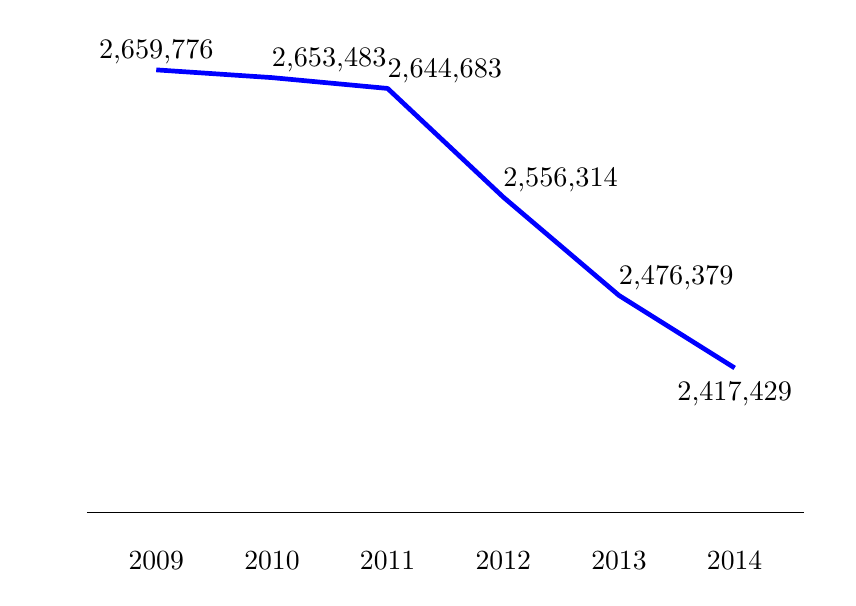
\begin{tikzpicture}[x=1pt,y=1pt]  % Created by tikzDevice version 0.9 on 2016-02-29 21:52:27
% !TEX encoding = UTF-8 Unicode
\definecolor{fillColor}{RGB}{255,255,255}
\path[use as bounding box,fill=fillColor,fill opacity=0.00] (0,0) rectangle (289.08,198.74);
\begin{scope}
\path[clip] (  0.00,  0.00) rectangle (289.08,198.74);

\path[] (  0.00,  0.00) rectangle (289.08,198.74);
\end{scope}
\begin{scope}
\path[clip] (  0.00,  0.00) rectangle (289.08,198.74);

\path[] ( 21.38, 15.61) rectangle (280.54,191.48);

\path[] ( 21.38, 45.83) --
	(280.54, 45.83);

\path[] ( 21.38, 90.27) --
	(280.54, 90.27);

\path[] ( 21.38,134.70) --
	(280.54,134.70);

\path[] ( 21.38,179.14) --
	(280.54,179.14);

\path[] ( 21.38, 23.61) --
	(280.54, 23.61);

\path[] ( 21.38, 68.05) --
	(280.54, 68.05);

\path[] ( 21.38,112.49) --
	(280.54,112.49);

\path[] ( 21.38,156.92) --
	(280.54,156.92);

\path[] ( 46.46, 15.61) --
	( 46.46,191.48);

\path[] ( 88.26, 15.61) --
	( 88.26,191.48);

\path[] (130.06, 15.61) --
	(130.06,191.48);

\path[] (171.86, 15.61) --
	(171.86,191.48);

\path[] (213.66, 15.61) --
	(213.66,191.48);

\path[] (255.46, 15.61) --
	(255.46,191.48);
\definecolor{drawColor}{RGB}{0,0,255}

\path[draw=drawColor,line width= 1.7pt,line join=round] ( 46.46,183.49) --
	( 88.26,180.69) --
	(130.06,176.78) --
	(171.86,137.51) --
	(213.66,101.99) --
	(255.46, 75.79);
\definecolor{drawColor}{RGB}{0,0,0}

\node[text=drawColor,anchor=base,inner sep=0pt, outer sep=0pt, scale=  1.02] at ( 46.46,187.46) {2,659,776};

\node[text=drawColor,anchor=base west,inner sep=0pt, outer sep=0pt, scale=  1.02] at ( 88.26,184.66) {2,653,483};

\node[text=drawColor,anchor=base west,inner sep=0pt, outer sep=0pt, scale=  1.02] at (130.06,180.75) {2,644,683};

\node[text=drawColor,anchor=base west,inner sep=0pt, outer sep=0pt, scale=  1.02] at (171.86,141.48) {2,556,314};

\node[text=drawColor,anchor=base west,inner sep=0pt, outer sep=0pt, scale=  1.02] at (213.66,105.96) {2,476,379};

\node[text=drawColor,anchor=base,inner sep=0pt, outer sep=0pt, scale=  1.02] at (255.46, 63.88) {2,417,429};

\path[draw=drawColor,line width= 0.1pt,line join=round] ( 21.38, 23.61) -- (280.54, 23.61);

\path[] ( 21.38, 15.61) rectangle (280.54,191.48);
\end{scope}
\begin{scope}
\path[clip] (  0.00,  0.00) rectangle (289.08,198.74);

\path[] ( 21.38, 15.61) --
	( 21.38,191.48);
\end{scope}
\begin{scope}
\path[clip] (  0.00,  0.00) rectangle (289.08,198.74);
\definecolor{drawColor}{RGB}{255,255,255}

\node[text=drawColor,text opacity=0.00,anchor=base east,inner sep=0pt, outer sep=0pt, scale=  1.00] at ( 16.43, 19.70) {2300000};

\node[text=drawColor,text opacity=0.00,anchor=base east,inner sep=0pt, outer sep=0pt, scale=  1.00] at ( 16.43, 64.14) {2400000};

\node[text=drawColor,text opacity=0.00,anchor=base east,inner sep=0pt, outer sep=0pt, scale=  1.00] at ( 16.43,108.58) {2500000};

\node[text=drawColor,text opacity=0.00,anchor=base east,inner sep=0pt, outer sep=0pt, scale=  1.00] at ( 16.43,153.02) {2600000};
\end{scope}
\begin{scope}
\path[clip] (  0.00,  0.00) rectangle (289.08,198.74);

\path[] ( 18.63, 23.61) --
	( 21.38, 23.61);

\path[] ( 18.63, 68.05) --
	( 21.38, 68.05);

\path[] ( 18.63,112.49) --
	( 21.38,112.49);

\path[] ( 18.63,156.92) --
	( 21.38,156.92);
\end{scope}
\begin{scope}
\path[clip] (  0.00,  0.00) rectangle (289.08,198.74);

\path[] ( 21.38, 15.61) --
	(280.54, 15.61);
\end{scope}
\begin{scope}
\path[clip] (  0.00,  0.00) rectangle (289.08,198.74);

\path[] ( 46.46, 12.86) --
	( 46.46, 15.61);

\path[] ( 88.26, 12.86) --
	( 88.26, 15.61);

\path[] (130.06, 12.86) --
	(130.06, 15.61);

\path[] (171.86, 12.86) --
	(171.86, 15.61);

\path[] (213.66, 12.86) --
	(213.66, 15.61);

\path[] (255.46, 12.86) --
	(255.46, 15.61);
\end{scope}
\begin{scope}
\path[clip] (  0.00,  0.00) rectangle (289.08,198.74);
\definecolor{drawColor}{RGB}{0,0,0}

\node[text=drawColor,anchor=base,inner sep=0pt, outer sep=0pt, scale=  1.00] at ( 46.46,  2.85) {2009};

\node[text=drawColor,anchor=base,inner sep=0pt, outer sep=0pt, scale=  1.00] at ( 88.26,  2.85) {2010};

\node[text=drawColor,anchor=base,inner sep=0pt, outer sep=0pt, scale=  1.00] at (130.06,  2.85) {2011};

\node[text=drawColor,anchor=base,inner sep=0pt, outer sep=0pt, scale=  1.00] at (171.86,  2.85) {2012};

\node[text=drawColor,anchor=base,inner sep=0pt, outer sep=0pt, scale=  1.00] at (213.66,  2.85) {2013};

\node[text=drawColor,anchor=base,inner sep=0pt, outer sep=0pt, scale=  1.00] at (255.46,  2.85) {2014};
\end{scope}
  \end{tikzpicture}}{Instituto Nacional de Estadística, con datos del Ministerio de Educación}

\cajita{Inscritos en primaria por sexo}{En la presente gráfica se observa que el porcentaje de hombres inscritos en primaria es 51.8\% y de mujeres  48.2\%.}{Distribución de inscritos en el ciclo de educación primaria, por sexo}{República de Guatemala, año 2014, en porcentaje}{\ \\[0mm]\begin{tikzpicture}[x=1pt,y=1pt]  % Created by tikzDevice version 0.9 on 2016-02-29 21:52:28
% !TEX encoding = UTF-8 Unicode
\definecolor{fillColor}{RGB}{255,255,255}
\path[use as bounding box,fill=fillColor,fill opacity=0.00] (0,0) rectangle (289.08,198.74);
\begin{scope}
\path[clip] ( 30.54,  0.00) rectangle (258.54,198.74);

\path[] ( 30.54,  0.00) rectangle (258.54,198.74);
\end{scope}
\begin{scope}
\path[clip] (  0.00,  0.00) rectangle (289.08,198.74);

\path[] (  7.11,  4.95) rectangle (200.91,198.74);

\path[] (104.01,101.85) --
	(191.08, 96.92);

\path[] (104.01,101.85) --
	( 16.94,106.77);

\path[] (104.01,101.85) --
	(108.94,188.91);

\path[] (104.01,101.85) --
	(191.08, 96.92);

\path[] (104.01,101.85) --
	( 99.08, 14.78);

\path[] (104.01,101.85) --
	( 16.94,106.77);

\path[] (104.01,101.85) --
	(104.01,101.85) --
	(104.01,101.85) --
	(104.01,101.85) --
	(104.01,101.85) --
	(104.01,101.85) --
	(104.01,101.85) --
	(104.01,101.85) --
	(104.01,101.85) --
	(104.01,101.85) --
	(104.01,101.85) --
	(104.01,101.85) --
	(104.01,101.85) --
	(104.01,101.85) --
	(104.01,101.85) --
	(104.01,101.85) --
	(104.01,101.85) --
	(104.01,101.85) --
	(104.01,101.85) --
	(104.01,101.85) --
	(104.01,101.85) --
	(104.01,101.85) --
	(104.01,101.85) --
	(104.01,101.85) --
	(104.01,101.85) --
	(104.01,101.85) --
	(104.01,101.85) --
	(104.01,101.85) --
	(104.01,101.85) --
	(104.01,101.85) --
	(104.01,101.85) --
	(104.01,101.85) --
	(104.01,101.85) --
	(104.01,101.85) --
	(104.01,101.85) --
	(104.01,101.85) --
	(104.01,101.85) --
	(104.01,101.85) --
	(104.01,101.85) --
	(104.01,101.85) --
	(104.01,101.85) --
	(104.01,101.85) --
	(104.01,101.85) --
	(104.01,101.85) --
	(104.01,101.85) --
	(104.01,101.85) --
	(104.01,101.85) --
	(104.01,101.85) --
	(104.01,101.85) --
	(104.01,101.85) --
	(104.01,101.85) --
	(104.01,101.85) --
	(104.01,101.85) --
	(104.01,101.85) --
	(104.01,101.85) --
	(104.01,101.85) --
	(104.01,101.85) --
	(104.01,101.85) --
	(104.01,101.85) --
	(104.01,101.85) --
	(104.01,101.85) --
	(104.01,101.85) --
	(104.01,101.85) --
	(104.01,101.85) --
	(104.01,101.85) --
	(104.01,101.85) --
	(104.01,101.85) --
	(104.01,101.85) --
	(104.01,101.85) --
	(104.01,101.85) --
	(104.01,101.85) --
	(104.01,101.85) --
	(104.01,101.85) --
	(104.01,101.85) --
	(104.01,101.85) --
	(104.01,101.85) --
	(104.01,101.85) --
	(104.01,101.85) --
	(104.01,101.85) --
	(104.01,101.85) --
	(104.01,101.85) --
	(104.01,101.85) --
	(104.01,101.85) --
	(104.01,101.85) --
	(104.01,101.85) --
	(104.01,101.85) --
	(104.01,101.85) --
	(104.01,101.85) --
	(104.01,101.85) --
	(104.01,101.85) --
	(104.01,101.85) --
	(104.01,101.85) --
	(104.01,101.85) --
	(104.01,101.85) --
	(104.01,101.85) --
	(104.01,101.85) --
	(104.01,101.85) --
	(104.01,101.85) --
	(104.01,101.85) --
	(104.01,101.85);

\path[] (104.01,121.23) --
	(105.24,121.19) --
	(106.46,121.07) --
	(107.68,120.88) --
	(108.88,120.60) --
	(110.06,120.26) --
	(111.21,119.84) --
	(112.34,119.34) --
	(113.43,118.78) --
	(114.49,118.15) --
	(115.50,117.45) --
	(116.47,116.69) --
	(117.38,115.87) --
	(118.25,115.00) --
	(119.05,114.07) --
	(119.80,113.09) --
	(120.48,112.06) --
	(121.09,111.00) --
	(121.64,109.90) --
	(122.11,108.76) --
	(122.51,107.60) --
	(122.84,106.42) --
	(123.09,105.21) --
	(123.27,103.99) --
	(123.37,102.77) --
	(123.39,101.54) --
	(123.33,100.31) --
	(123.19, 99.09) --
	(122.98, 97.88) --
	(122.69, 96.68) --
	(122.32, 95.51) --
	(121.88, 94.36) --
	(121.37, 93.24) --
	(120.79, 92.16) --
	(120.14, 91.11) --
	(119.43, 90.11) --
	(118.66, 89.16) --
	(117.82, 88.25) --
	(116.93, 87.40) --
	(115.99, 86.61) --
	(115.00, 85.88) --
	(113.96, 85.22) --
	(112.89, 84.62) --
	(111.78, 84.09) --
	(110.64, 83.64) --
	(109.47, 83.25) --
	(108.28, 82.94) --
	(107.07, 82.71) --
	(105.85, 82.55) --
	(104.62, 82.48) --
	(103.39, 82.48) --
	(102.17, 82.55) --
	(100.95, 82.71) --
	( 99.74, 82.94) --
	( 98.55, 83.25) --
	( 97.38, 83.64) --
	( 96.24, 84.09) --
	( 95.13, 84.62) --
	( 94.05, 85.22) --
	( 93.02, 85.88) --
	( 92.03, 86.61) --
	( 91.09, 87.40) --
	( 90.20, 88.25) --
	( 89.36, 89.16) --
	( 88.59, 90.11) --
	( 87.87, 91.11) --
	( 87.23, 92.16) --
	( 86.65, 93.24) --
	( 86.13, 94.36) --
	( 85.70, 95.51) --
	( 85.33, 96.68) --
	( 85.04, 97.88) --
	( 84.83, 99.09) --
	( 84.69,100.31) --
	( 84.63,101.54) --
	( 84.65,102.77) --
	( 84.75,103.99) --
	( 84.92,105.21) --
	( 85.18,106.42) --
	( 85.50,107.60) --
	( 85.91,108.76) --
	( 86.38,109.90) --
	( 86.93,111.00) --
	( 87.54,112.06) --
	( 88.22,113.09) --
	( 88.97,114.07) --
	( 89.77,115.00) --
	( 90.64,115.87) --
	( 91.55,116.69) --
	( 92.52,117.45) --
	( 93.53,118.15) --
	( 94.59,118.78) --
	( 95.68,119.34) --
	( 96.81,119.84) --
	( 97.96,120.26) --
	( 99.14,120.60) --
	(100.34,120.88) --
	(101.56,121.07) --
	(102.78,121.19) --
	(104.01,121.23);

\path[] (104.01,140.60) --
	(106.47,140.53) --
	(108.92,140.29) --
	(111.34,139.90) --
	(113.74,139.36) --
	(116.10,138.67) --
	(118.41,137.83) --
	(120.67,136.84) --
	(122.85,135.72) --
	(124.96,134.45) --
	(126.99,133.06) --
	(128.92,131.54) --
	(130.76,129.90) --
	(132.48,128.14) --
	(134.09,126.29) --
	(135.58,124.33) --
	(136.94,122.28) --
	(138.17,120.15) --
	(139.27,117.95) --
	(140.22,115.68) --
	(141.02,113.35) --
	(141.68,110.98) --
	(142.18,108.58) --
	(142.53,106.14) --
	(142.72,103.69) --
	(142.76,101.23) --
	(142.65, 98.77) --
	(142.37, 96.33) --
	(141.95, 93.91) --
	(141.37, 91.52) --
	(140.64, 89.17) --
	(139.76, 86.87) --
	(138.74, 84.63) --
	(137.58, 82.47) --
	(136.28, 80.38) --
	(134.85, 78.37) --
	(133.30, 76.46) --
	(131.63, 74.66) --
	(129.85, 72.96) --
	(127.97, 71.38) --
	(125.99, 69.92) --
	(123.92, 68.59) --
	(121.77, 67.40) --
	(119.55, 66.34) --
	(117.27, 65.43) --
	(114.93, 64.66) --
	(112.55, 64.04) --
	(110.13, 63.57) --
	(107.69, 63.26) --
	(105.24, 63.11) --
	(102.78, 63.11) --
	(100.33, 63.26) --
	( 97.89, 63.57) --
	( 95.47, 64.04) --
	( 93.09, 64.66) --
	( 90.75, 65.43) --
	( 88.47, 66.34) --
	( 86.25, 67.40) --
	( 84.10, 68.59) --
	( 82.03, 69.92) --
	( 80.05, 71.38) --
	( 78.17, 72.96) --
	( 76.39, 74.66) --
	( 74.72, 76.46) --
	( 73.17, 78.37) --
	( 71.74, 80.38) --
	( 70.44, 82.47) --
	( 69.28, 84.63) --
	( 68.26, 86.87) --
	( 67.38, 89.17) --
	( 66.65, 91.52) --
	( 66.07, 93.91) --
	( 65.65, 96.33) --
	( 65.37, 98.77) --
	( 65.26,101.23) --
	( 65.29,103.69) --
	( 65.49,106.14) --
	( 65.84,108.58) --
	( 66.34,110.98) --
	( 67.00,113.35) --
	( 67.80,115.68) --
	( 68.75,117.95) --
	( 69.85,120.15) --
	( 71.08,122.28) --
	( 72.44,124.33) --
	( 73.93,126.29) --
	( 75.54,128.14) --
	( 77.26,129.90) --
	( 79.10,131.54) --
	( 81.03,133.06) --
	( 83.06,134.45) --
	( 85.17,135.72) --
	( 87.35,136.84) --
	( 89.60,137.83) --
	( 91.92,138.67) --
	( 94.28,139.36) --
	( 96.67,139.90) --
	( 99.10,140.29) --
	(101.55,140.53) --
	(104.01,140.60);

\path[] (104.01,159.98) --
	(107.70,159.87) --
	(111.37,159.52) --
	(115.01,158.93) --
	(118.61,158.12) --
	(122.15,157.08) --
	(125.62,155.82) --
	(129.00,154.34) --
	(132.28,152.65) --
	(135.44,150.75) --
	(138.48,148.66) --
	(141.38,146.38) --
	(144.13,143.92) --
	(146.72,141.29) --
	(149.13,138.51) --
	(151.37,135.57) --
	(153.41,132.50) --
	(155.26,129.30) --
	(156.89,126.00) --
	(158.32,122.59) --
	(159.53,119.11) --
	(160.51,115.55) --
	(161.26,111.94) --
	(161.79,108.29) --
	(162.08,104.61) --
	(162.14,100.92) --
	(161.96, 97.24) --
	(161.56, 93.57) --
	(160.91, 89.94) --
	(160.05, 86.35) --
	(158.95, 82.83) --
	(157.63, 79.39) --
	(156.10, 76.03) --
	(154.36, 72.78) --
	(152.41, 69.64) --
	(150.27, 66.64) --
	(147.95, 63.77) --
	(145.44, 61.06) --
	(142.77, 58.52) --
	(139.95, 56.15) --
	(136.98, 53.96) --
	(133.87, 51.97) --
	(130.65, 50.17) --
	(127.32, 48.59) --
	(123.89, 47.21) --
	(120.39, 46.06) --
	(116.82, 45.14) --
	(113.20, 44.44) --
	(109.54, 43.97) --
	(105.85, 43.74) --
	(102.16, 43.74) --
	( 98.48, 43.97) --
	( 94.82, 44.44) --
	( 91.20, 45.14) --
	( 87.63, 46.06) --
	( 84.13, 47.21) --
	( 80.70, 48.59) --
	( 77.37, 50.17) --
	( 74.15, 51.97) --
	( 71.04, 53.96) --
	( 68.07, 56.15) --
	( 65.25, 58.52) --
	( 62.58, 61.06) --
	( 60.07, 63.77) --
	( 57.75, 66.64) --
	( 55.61, 69.64) --
	( 53.66, 72.78) --
	( 51.92, 76.03) --
	( 50.39, 79.39) --
	( 49.07, 82.83) --
	( 47.97, 86.35) --
	( 47.10, 89.94) --
	( 46.46, 93.57) --
	( 46.05, 97.24) --
	( 45.88,100.92) --
	( 45.94,104.61) --
	( 46.23,108.29) --
	( 46.75,111.94) --
	( 47.51,115.55) --
	( 48.49,119.11) --
	( 49.70,122.59) --
	( 51.13,126.00) --
	( 52.76,129.30) --
	( 54.61,132.50) --
	( 56.65,135.57) --
	( 58.89,138.51) --
	( 61.30,141.29) --
	( 63.89,143.92) --
	( 66.64,146.38) --
	( 69.54,148.66) --
	( 72.58,150.75) --
	( 75.74,152.65) --
	( 79.02,154.34) --
	( 82.40,155.82) --
	( 85.87,157.08) --
	( 89.41,158.12) --
	( 93.01,158.93) --
	( 96.65,159.52) --
	(100.32,159.87) --
	(104.01,159.98);

\path[] (104.01,179.36) --
	(108.93,179.21) --
	(113.82,178.74) --
	(118.68,177.96) --
	(123.48,176.88) --
	(128.20,175.49) --
	(132.82,173.81) --
	(137.33,171.84) --
	(141.70,169.58) --
	(145.92,167.06) --
	(149.97,164.27) --
	(153.84,161.23) --
	(157.50,157.95) --
	(160.95,154.44) --
	(164.17,150.72) --
	(167.15,146.81) --
	(169.88,142.72) --
	(172.34,138.46) --
	(174.52,134.05) --
	(176.42,129.51) --
	(178.03,124.86) --
	(179.34,120.12) --
	(180.35,115.31) --
	(181.05,110.44) --
	(181.44,105.53) --
	(181.52,100.62) --
	(181.28, 95.70) --
	(180.74, 90.81) --
	(179.88, 85.97) --
	(178.72, 81.19) --
	(177.26, 76.49) --
	(175.51, 71.90) --
	(173.46, 67.42) --
	(171.14, 63.09) --
	(168.55, 58.91) --
	(165.69, 54.90) --
	(162.59, 51.08) --
	(159.26, 47.47) --
	(155.70, 44.08) --
	(151.93, 40.91) --
	(147.97, 38.00) --
	(143.83, 35.34) --
	(139.53, 32.95) --
	(135.09, 30.83) --
	(130.52, 29.00) --
	(125.85, 27.47) --
	(121.09, 26.23) --
	(116.26, 25.30) --
	(111.38, 24.68) --
	(106.47, 24.37) --
	(101.55, 24.37) --
	( 96.64, 24.68) --
	( 91.76, 25.30) --
	( 86.93, 26.23) --
	( 82.17, 27.47) --
	( 77.50, 29.00) --
	( 72.93, 30.83) --
	( 68.49, 32.95) --
	( 64.19, 35.34) --
	( 60.05, 38.00) --
	( 56.09, 40.91) --
	( 52.32, 44.08) --
	( 48.76, 47.47) --
	( 45.43, 51.08) --
	( 42.32, 54.90) --
	( 39.47, 58.91) --
	( 36.88, 63.09) --
	( 34.55, 67.42) --
	( 32.51, 71.90) --
	( 30.76, 76.49) --
	( 29.30, 81.19) --
	( 28.14, 85.97) --
	( 27.28, 90.81) --
	( 26.74, 95.70) --
	( 26.50,100.62) --
	( 26.58,105.53) --
	( 26.97,110.44) --
	( 27.67,115.31) --
	( 28.68,120.12) --
	( 29.99,124.86) --
	( 31.60,129.51) --
	( 33.50,134.05) --
	( 35.68,138.46) --
	( 38.14,142.72) --
	( 40.87,146.81) --
	( 43.84,150.72) --
	( 47.07,154.44) --
	( 50.52,157.95) --
	( 54.18,161.23) --
	( 58.05,164.27) --
	( 62.10,167.06) --
	( 66.32,169.58) --
	( 70.69,171.84) --
	( 75.20,173.81) --
	( 79.82,175.49) --
	( 84.54,176.88) --
	( 89.34,177.96) --
	( 94.20,178.74) --
	( 99.09,179.21) --
	(104.01,179.36);

\path[] (104.01,189.05) --
	(109.54,188.88) --
	(115.05,188.35) --
	(120.51,187.48) --
	(125.91,186.26) --
	(131.22,184.70) --
	(136.42,182.81) --
	(141.49,180.59) --
	(146.41,178.05) --
	(151.16,175.21) --
	(155.71,172.07) --
	(160.06,168.65) --
	(164.19,164.96) --
	(168.07,161.02) --
	(171.69,156.83) --
	(175.05,152.43) --
	(178.11,147.82) --
	(180.88,143.03) --
	(183.34,138.07) --
	(185.47,132.97) --
	(187.28,127.74) --
	(188.76,122.41) --
	(189.89,116.99) --
	(190.68,111.51) --
	(191.12,106.00) --
	(191.21,100.46) --
	(190.94, 94.94) --
	(190.33, 89.44) --
	(189.37, 83.99) --
	(188.06, 78.61) --
	(186.42, 73.32) --
	(184.44, 68.15) --
	(182.15, 63.12) --
	(179.53, 58.24) --
	(176.62, 53.54) --
	(173.41, 49.03) --
	(169.92, 44.74) --
	(166.16, 40.67) --
	(162.16, 36.85) --
	(157.92, 33.30) --
	(153.46, 30.02) --
	(148.81, 27.02) --
	(143.97, 24.33) --
	(138.97, 21.96) --
	(133.84, 19.90) --
	(128.58, 18.17) --
	(123.22, 16.78) --
	(117.79, 15.74) --
	(112.30, 15.03) --
	(106.78, 14.68) --
	(101.24, 14.68) --
	( 95.72, 15.03) --
	( 90.23, 15.74) --
	( 84.80, 16.78) --
	( 79.44, 18.17) --
	( 74.18, 19.90) --
	( 69.05, 21.96) --
	( 64.05, 24.33) --
	( 59.21, 27.02) --
	( 54.56, 30.02) --
	( 50.10, 33.30) --
	( 45.86, 36.85) --
	( 41.86, 40.67) --
	( 38.10, 44.74) --
	( 34.61, 49.03) --
	( 31.40, 53.54) --
	( 28.49, 58.24) --
	( 25.87, 63.12) --
	( 23.57, 68.15) --
	( 21.60, 73.32) --
	( 19.96, 78.61) --
	( 18.65, 83.99) --
	( 17.69, 89.44) --
	( 17.08, 94.94) --
	( 16.81,100.46) --
	( 16.90,106.00) --
	( 17.34,111.51) --
	( 18.13,116.99) --
	( 19.26,122.41) --
	( 20.74,127.74) --
	( 22.55,132.97) --
	( 24.68,138.07) --
	( 27.14,143.03) --
	( 29.91,147.82) --
	( 32.97,152.43) --
	( 36.32,156.83) --
	( 39.95,161.02) --
	( 43.83,164.96) --
	( 47.95,168.65) --
	( 52.30,172.07) --
	( 56.86,175.21) --
	( 61.61,178.05) --
	( 66.53,180.59) --
	( 71.60,182.81) --
	( 76.80,184.70) --
	( 82.11,186.26) --
	( 87.51,187.48) --
	( 92.97,188.35) --
	( 98.48,188.88) --
	(104.01,189.05);
\definecolor{drawColor}{RGB}{255,255,255}
\definecolor{fillColor}{RGB}{0,0,255}

\path[draw=drawColor,line width= 0.6pt,line join=round,line cap=round,fill=fillColor] ( 99.64, 63.34) --
	( 99.32, 60.58) --
	( 99.01, 57.83) --
	( 98.70, 55.08) --
	( 98.39, 52.33) --
	( 98.07, 49.58) --
	( 97.76, 46.83) --
	( 97.45, 44.08) --
	( 97.14, 41.33) --
	( 96.83, 38.58) --
	( 96.51, 35.83) --
	( 96.20, 33.08) --
	( 95.89, 30.33) --
	( 95.58, 27.58) --
	( 95.26, 24.82) --
	( 97.88, 24.57) --
	(100.50, 24.41) --
	(103.13, 24.33) --
	(105.76, 24.35) --
	(108.38, 24.45) --
	(111.00, 24.65) --
	(113.62, 24.93) --
	(116.22, 25.30) --
	(118.81, 25.75) --
	(121.38, 26.30) --
	(123.93, 26.93) --
	(126.45, 27.65) --
	(128.96, 28.45) --
	(131.43, 29.34) --
	(133.87, 30.31) --
	(136.28, 31.37) --
	(138.65, 32.50) --
	(140.98, 33.71) --
	(143.27, 35.01) --
	(145.51, 36.38) --
	(147.71, 37.82) --
	(149.85, 39.34) --
	(151.95, 40.93) --
	(153.98, 42.59) --
	(155.96, 44.32) --
	(157.88, 46.11) --
	(159.74, 47.97) --
	(161.54, 49.89) --
	(163.26, 51.87) --
	(164.92, 53.90) --
	(166.51, 56.00) --
	(168.03, 58.14) --
	(169.48, 60.34) --
	(170.85, 62.58) --
	(172.14, 64.87) --
	(173.35, 67.20) --
	(174.49, 69.57) --
	(175.54, 71.98) --
	(176.51, 74.42) --
	(177.40, 76.89) --
	(178.20, 79.39) --
	(178.92, 81.92) --
	(179.55, 84.47) --
	(180.10, 87.04) --
	(180.56, 89.63) --
	(180.93, 92.23) --
	(181.21, 94.85) --
	(181.40, 97.47) --
	(181.51,100.09) --
	(181.52,102.72) --
	(181.45,105.35) --
	(181.28,107.97) --
	(181.03,110.59) --
	(180.69,113.19) --
	(180.26,115.78) --
	(179.75,118.36) --
	(179.14,120.92) --
	(178.45,123.45) --
	(177.68,125.97) --
	(176.82,128.45) --
	(175.88,130.90) --
	(174.85,133.32) --
	(173.74,135.70) --
	(172.55,138.05) --
	(171.29,140.35) --
	(169.94,142.61) --
	(168.52,144.82) --
	(167.03,146.98) --
	(165.46,149.09) --
	(163.83,151.15) --
	(162.12,153.15) --
	(160.35,155.09) --
	(158.51,156.97) --
	(156.61,158.78) --
	(154.65,160.53) --
	(152.63,162.22) --
	(150.56,163.83) --
	(148.43,165.37) --
	(146.25,166.84) --
	(144.03,168.24) --
	(141.75,169.55) --
	(139.44,170.79) --
	(137.08,171.96) --
	(134.68,173.04) --
	(132.25,174.04) --
	(129.79,174.95) --
	(127.30,175.78) --
	(124.78,176.53) --
	(122.23,177.19) --
	(119.67,177.77) --
	(117.09,178.25) --
	(114.49,178.65) --
	(111.88,178.96) --
	(109.26,179.19) --
	(106.64,179.32) --
	(104.01,179.36) --
	(104.01,176.59) --
	(104.01,173.83) --
	(104.01,171.06) --
	(104.01,168.29) --
	(104.01,165.52) --
	(104.01,162.75) --
	(104.01,159.98) --
	(104.01,157.22) --
	(104.01,154.45) --
	(104.01,151.68) --
	(104.01,148.91) --
	(104.01,146.14) --
	(104.01,143.37) --
	(104.01,140.60) --
	(106.64,140.52) --
	(109.25,140.25) --
	(111.84,139.81) --
	(114.39,139.19) --
	(116.90,138.40) --
	(119.35,137.44) --
	(121.72,136.32) --
	(124.02,135.04) --
	(126.22,133.61) --
	(128.32,132.03) --
	(130.31,130.31) --
	(132.18,128.47) --
	(133.92,126.50) --
	(135.52,124.41) --
	(136.98,122.23) --
	(138.28,119.95) --
	(139.43,117.58) --
	(140.41,115.15) --
	(141.23,112.65) --
	(141.88,110.10) --
	(142.35,107.52) --
	(142.65,104.91) --
	(142.77,102.28) --
	(142.71, 99.66) --
	(142.47, 97.04) --
	(142.05, 94.44) --
	(141.47, 91.88) --
	(140.70, 89.37) --
	(139.78, 86.91) --
	(138.68, 84.52) --
	(137.43, 82.21) --
	(136.02, 79.99) --
	(134.47, 77.88) --
	(132.77, 75.87) --
	(130.95, 73.98) --
	(129.00, 72.22) --
	(126.93, 70.59) --
	(124.76, 69.11) --
	(122.50, 67.78) --
	(120.14, 66.61) --
	(117.72, 65.59) --
	(115.23, 64.75) --
	(112.69, 64.07) --
	(110.11, 63.57) --
	(107.51, 63.25) --
	(104.88, 63.10) --
	(102.26, 63.13) --
	( 99.64, 63.34) --
	cycle;
\definecolor{fillColor}{RGB}{157,187,255}

\path[draw=drawColor,line width= 0.6pt,line join=round,line cap=round,fill=fillColor] (104.01,140.60) --
	(104.01,143.37) --
	(104.01,146.14) --
	(104.01,148.91) --
	(104.01,151.68) --
	(104.01,154.45) --
	(104.01,157.22) --
	(104.01,159.98) --
	(104.01,162.75) --
	(104.01,165.52) --
	(104.01,168.29) --
	(104.01,171.06) --
	(104.01,173.83) --
	(104.01,176.59) --
	(104.01,179.36) --
	(101.37,179.32) --
	( 98.74,179.18) --
	( 96.11,178.96) --
	( 93.49,178.65) --
	( 90.88,178.24) --
	( 88.29,177.75) --
	( 85.72,177.17) --
	( 83.17,176.51) --
	( 80.64,175.76) --
	( 78.14,174.92) --
	( 75.67,174.00) --
	( 73.23,172.99) --
	( 70.83,171.90) --
	( 68.46,170.73) --
	( 66.14,169.48) --
	( 63.86,168.16) --
	( 61.63,166.75) --
	( 59.44,165.27) --
	( 57.31,163.72) --
	( 55.23,162.09) --
	( 53.21,160.40) --
	( 51.25,158.64) --
	( 49.35,156.81) --
	( 47.51,154.92) --
	( 45.74,152.96) --
	( 44.03,150.95) --
	( 42.39,148.88) --
	( 40.83,146.76) --
	( 39.34,144.58) --
	( 37.92,142.36) --
	( 36.58,140.09) --
	( 35.32,137.77) --
	( 34.14,135.41) --
	( 33.04,133.02) --
	( 32.02,130.58) --
	( 31.08,128.12) --
	( 30.23,125.62) --
	( 29.46,123.10) --
	( 28.78,120.55) --
	( 28.19,117.98) --
	( 27.69,115.39) --
	( 27.27,112.79) --
	( 26.94,110.17) --
	( 26.70,107.54) --
	( 26.55,104.91) --
	( 26.49,102.27) --
	( 26.52, 99.63) --
	( 26.64, 97.00) --
	( 26.85, 94.37) --
	( 27.15, 91.75) --
	( 27.54, 89.14) --
	( 28.02, 86.55) --
	( 28.58, 83.97) --
	( 29.23, 81.41) --
	( 29.97, 78.88) --
	( 30.80, 76.38) --
	( 31.71, 73.90) --
	( 32.70, 71.46) --
	( 33.77, 69.05) --
	( 34.93, 66.68) --
	( 36.17, 64.35) --
	( 37.48, 62.06) --
	( 38.87, 59.82) --
	( 40.34, 57.63) --
	( 41.88, 55.49) --
	( 43.49, 53.40) --
	( 45.18, 51.37) --
	( 46.93, 49.40) --
	( 48.75, 47.49) --
	( 50.63, 45.64) --
	( 52.57, 43.85) --
	( 54.57, 42.14) --
	( 56.63, 40.49) --
	( 58.75, 38.91) --
	( 60.92, 37.41) --
	( 63.13, 35.98) --
	( 65.40, 34.63) --
	( 67.71, 33.36) --
	( 70.06, 32.16) --
	( 72.45, 31.05) --
	( 74.88, 30.01) --
	( 77.34, 29.06) --
	( 79.83, 28.20) --
	( 82.35, 27.42) --
	( 84.89, 26.72) --
	( 87.46, 26.12) --
	( 90.05, 25.60) --
	( 92.65, 25.17) --
	( 95.26, 24.82) --
	( 95.58, 27.58) --
	( 95.89, 30.33) --
	( 96.20, 33.08) --
	( 96.51, 35.83) --
	( 96.83, 38.58) --
	( 97.14, 41.33) --
	( 97.45, 44.08) --
	( 97.76, 46.83) --
	( 98.07, 49.58) --
	( 98.39, 52.33) --
	( 98.70, 55.08) --
	( 99.01, 57.83) --
	( 99.32, 60.58) --
	( 99.64, 63.34) --
	( 97.00, 63.73) --
	( 94.39, 64.30) --
	( 91.83, 65.05) --
	( 89.33, 65.97) --
	( 86.90, 67.07) --
	( 84.55, 68.33) --
	( 82.29, 69.75) --
	( 80.13, 71.32) --
	( 78.09, 73.03) --
	( 76.17, 74.88) --
	( 74.38, 76.86) --
	( 72.73, 78.96) --
	( 71.23, 81.16) --
	( 69.89, 83.47) --
	( 68.70, 85.86) --
	( 67.69, 88.32) --
	( 66.84, 90.85) --
	( 66.17, 93.43) --
	( 65.69, 96.06) --
	( 65.38, 98.71) --
	( 65.25,101.37) --
	( 65.31,104.04) --
	( 65.56,106.69) --
	( 65.98,109.33) --
	( 66.58,111.92) --
	( 67.37,114.47) --
	( 68.32,116.96) --
	( 69.45,119.38) --
	( 70.73,121.72) --
	( 72.18,123.96) --
	( 73.77,126.10) --
	( 75.51,128.12) --
	( 77.39,130.02) --
	( 79.39,131.78) --
	( 81.51,133.40) --
	( 83.73,134.88) --
	( 86.05,136.19) --
	( 88.45,137.35) --
	( 90.93,138.33) --
	( 93.47,139.15) --
	( 96.06,139.78) --
	( 98.69,140.24) --
	(101.34,140.51) --
	(104.01,140.60) --
	cycle;
\definecolor{drawColor}{RGB}{0,0,0}

\node[text=drawColor,anchor=base,inner sep=0pt, outer sep=0pt, scale=  1.00] at (191.08, 93.01) {51.8};

\node[text=drawColor,anchor=base,inner sep=0pt, outer sep=0pt, scale=  1.00] at ( 16.94,102.87) {48.2};

\path[] (  7.11,  4.95) rectangle (200.91,198.74);
\end{scope}
\begin{scope}
\path[clip] (  0.00,  0.00) rectangle (289.08,198.74);

\path[] (  7.11,  4.95) --
	(  7.11,198.74);
\end{scope}
\begin{scope}
\path[clip] (  0.00,  0.00) rectangle (289.08,198.74);

\path[] (  4.36,101.85) --
	(  7.11,101.85);

\path[] (  4.36,121.23) --
	(  7.11,121.23);

\path[] (  4.36,140.60) --
	(  7.11,140.60);

\path[] (  4.36,159.98) --
	(  7.11,159.98);

\path[] (  4.36,179.36) --
	(  7.11,179.36);
\end{scope}
\begin{scope}
\path[clip] (  0.00,  0.00) rectangle (289.08,198.74);

\path[] (  7.11,  4.95) --
	(200.91,  4.95);
\end{scope}
\begin{scope}
\path[clip] (  0.00,  0.00) rectangle (289.08,198.74);
\coordinate (rect) at (192.72,99.37);
\coordinate (desY) at (0,18.49);
\coordinate (desX) at (7.11,11.38);
\coordinate (mdesX) at (7.11,-11.38);
\definecolor[named]{ct1}{HTML}{
0000FF
}
\definecolor[named]{borde}{HTML}{
0000FF
}
\coordinate (t1) at ($(rect) + 0.5*(desX) + 0.5*(desY)$);
\coordinate (t2) at ($(rect)+0.5*(mdesX)-0.5*(desY)$);
\draw [color=ct1,fill=borde] ($(rect)+(desY)$) rectangle ($(rect)+(desX)$);
\definecolor[named]{ct2}{HTML}{
9DBBFF
}
\node [text width=
56.692913328
,right= 0.3cm of t1,scale = 0.9]{
Hombre
};
\path [fill=ct2] ($(rect)-(desY)$) rectangle ($(rect)+(mdesX)$);
\node [text width=
56.692913328
,right= 0.3cm of t2,scale = 0.9]{
Mujer
};
\end{scope}
  \end{tikzpicture}}{Instituto Nacional de Estadística, con datos del Ministerio de Educación}

\cajita{Inscritos en primaria por grado}{La presente gráfica desagrega a los inscritos en educación primaria según el grado de estudio.
	
La mayor cantidad de alumnos se concentra en el primer grado, con el 20.2\% y, según esta relación, el 13.9\% se inscribió en sexto grado.}{Distribución porcentual de inscritos en el ciclo de educación primaria, según el grado escolar}{República de Guatemala, año 2014, en porcentaje}{\ \\[0mm]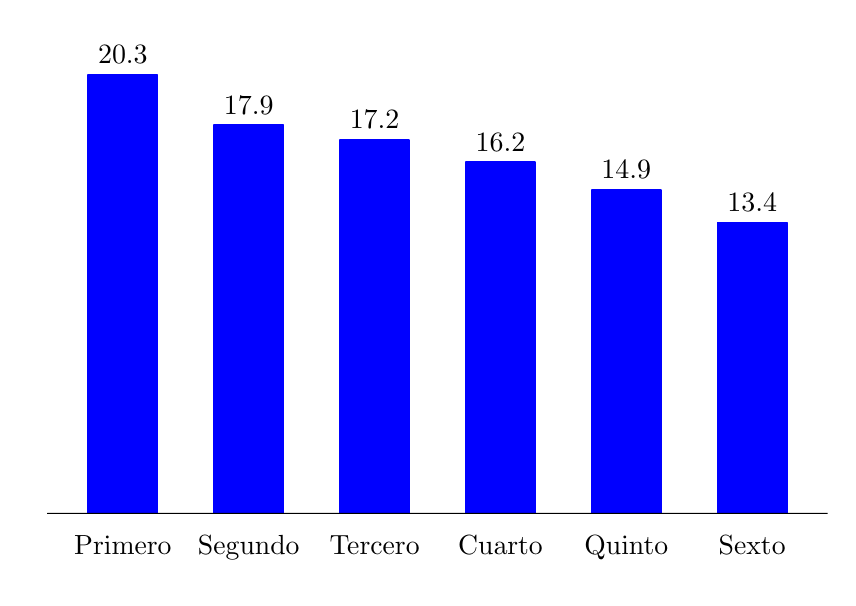
\begin{tikzpicture}[x=1pt,y=1pt]  % Created by tikzDevice version 0.7.0 on 2015-08-31 18:13:42
% !TEX encoding = UTF-8 Unicode
\definecolor[named]{fillColor}{rgb}{1.00,1.00,1.00}
\path[use as bounding box,fill=fillColor,fill opacity=0.00] (0,0) rectangle (289.08,198.74);
\begin{scope}
\path[clip] (  0.00,  0.00) rectangle (289.08,198.74);
\definecolor[named]{drawColor}{rgb}{1.00,1.00,1.00}

\path[draw=drawColor,line width= 0.6pt,line join=round,line cap=round] (  0.00,  0.00) rectangle (289.08,198.74);
\end{scope}
\begin{scope}
\path[clip] (  0.00,  0.00) rectangle (289.08,198.74);

\path[] (  7.11, 23.47) rectangle (289.08,181.67);

\path[] ( 34.40, 23.47) --
	( 34.40,181.67);

\path[] ( 79.88, 23.47) --
	( 79.88,181.67);

\path[] (125.36, 23.47) --
	(125.36,181.67);

\path[] (170.84, 23.47) --
	(170.84,181.67);

\path[] (216.31, 23.47) --
	(216.31,181.67);

\path[] (261.79, 23.47) --
	(261.79,181.67);
\definecolor[named]{drawColor}{rgb}{0.00,0.00,1.00}
\definecolor[named]{fillColor}{rgb}{0.00,0.00,1.00}

\path[draw=drawColor,line width= 0.6pt,line join=round,fill=fillColor] ( 21.89, 23.47) rectangle ( 46.91,181.67);

\path[draw=drawColor,line width= 0.6pt,line join=round,fill=fillColor] ( 67.37, 23.47) rectangle ( 92.39,163.57);

\path[draw=drawColor,line width= 0.6pt,line join=round,fill=fillColor] (112.85, 23.47) rectangle (137.86,158.20);

\path[draw=drawColor,line width= 0.6pt,line join=round,fill=fillColor] (158.33, 23.47) rectangle (183.34,150.15);

\path[draw=drawColor,line width= 0.6pt,line join=round,fill=fillColor] (203.81, 23.47) rectangle (228.82,140.16);

\path[draw=drawColor,line width= 0.6pt,line join=round,fill=fillColor] (249.29, 23.47) rectangle (274.30,128.28);
\definecolor[named]{drawColor}{rgb}{0.00,0.00,0.00}
\definecolor[named]{fillColor}{rgb}{0.00,0.00,0.00}

\path[draw=drawColor,line width= 0.1pt,line join=round,fill=fillColor] (  7.11, 23.47) -- (289.08, 23.47);

\node[text=drawColor,anchor=base,inner sep=0pt, outer sep=0pt, scale=  1.01] at ( 34.40,185.63) {20.3};

\node[text=drawColor,anchor=base,inner sep=0pt, outer sep=0pt, scale=  1.01] at ( 79.88,167.53) {17.9};

\node[text=drawColor,anchor=base,inner sep=0pt, outer sep=0pt, scale=  1.01] at (125.36,162.15) {17.2};

\node[text=drawColor,anchor=base,inner sep=0pt, outer sep=0pt, scale=  1.01] at (170.84,154.10) {16.2};

\node[text=drawColor,anchor=base,inner sep=0pt, outer sep=0pt, scale=  1.01] at (216.31,144.11) {14.9};

\node[text=drawColor,anchor=base,inner sep=0pt, outer sep=0pt, scale=  1.01] at (261.79,132.24) {13.4};
\end{scope}
\begin{scope}
\path[clip] (  0.00,  0.00) rectangle (289.08,198.74);

\path[] (  7.11, 23.47) --
	(  7.11,181.67);
\end{scope}
\begin{scope}
\path[clip] (  0.00,  0.00) rectangle (289.08,198.74);

\path[] (  7.11, 23.47) --
	(289.08, 23.47);
\end{scope}
\begin{scope}
\path[clip] (  0.00,  0.00) rectangle (289.08,198.74);

\path[] ( 34.40, 19.20) --
	( 34.40, 23.47);

\path[] ( 79.88, 19.20) --
	( 79.88, 23.47);

\path[] (125.36, 19.20) --
	(125.36, 23.47);

\path[] (170.84, 19.20) --
	(170.84, 23.47);

\path[] (216.31, 19.20) --
	(216.31, 23.47);

\path[] (261.79, 19.20) --
	(261.79, 23.47);
\end{scope}
\begin{scope}
\path[clip] (  0.00,  0.00) rectangle (289.08,198.74);
\definecolor[named]{drawColor}{rgb}{0.00,0.00,0.00}

\node[text=drawColor,anchor=base,inner sep=0pt, outer sep=0pt, scale=  1.00] at ( 34.40,  8.54) {Primero};

\node[text=drawColor,anchor=base,inner sep=0pt, outer sep=0pt, scale=  1.00] at ( 79.88,  8.54) {Segundo};

\node[text=drawColor,anchor=base,inner sep=0pt, outer sep=0pt, scale=  1.00] at (125.36,  8.54) {Tercero};

\node[text=drawColor,anchor=base,inner sep=0pt, outer sep=0pt, scale=  1.00] at (170.84,  8.54) {Cuarto};

\node[text=drawColor,anchor=base,inner sep=0pt, outer sep=0pt, scale=  1.00] at (216.31,  8.54) {Quinto};

\node[text=drawColor,anchor=base,inner sep=0pt, outer sep=0pt, scale=  1.00] at (261.79,  8.54) {Sexto};
\end{scope}
  \end{tikzpicture}}{Instituto Nacional de Estadística, con datos del Ministerio de Educación}

\cajita{Inscritos en primaria por etnia}{En la presente gráfica se observa que del total de inscritos en primaria, los no indígenas representaron el 61.4\%.}{Distribución de inscritos en el ciclo de educación primaria,\\ por grupo étnico}{República de Guatemala, año 2014, en porcentaje}{\ \\[0mm]\begin{tikzpicture}[x=1pt,y=1pt]  % Created by tikzDevice version 0.9 on 2016-02-29 21:52:28
% !TEX encoding = UTF-8 Unicode
\definecolor{fillColor}{RGB}{255,255,255}
\path[use as bounding box,fill=fillColor,fill opacity=0.00] (0,0) rectangle (289.08,198.74);
\begin{scope}
\path[clip] ( 30.54,  0.00) rectangle (258.54,198.74);

\path[] ( 30.54,  0.00) rectangle (258.54,198.74);
\end{scope}
\begin{scope}
\path[clip] (  0.00,  0.00) rectangle (289.08,198.74);

\path[] (  7.11,  4.95) rectangle (200.91,198.74);

\path[] (104.01,101.85) --
	(185.71, 71.34);

\path[] (104.01,101.85) --
	( 22.31,132.35);

\path[] (104.01,101.85) --
	(134.52,183.54);

\path[] (104.01,101.85) --
	(185.71, 71.34);

\path[] (104.01,101.85) --
	( 73.50, 20.15);

\path[] (104.01,101.85) --
	( 22.31,132.35);

\path[] (104.01,101.85) --
	(104.01,101.85) --
	(104.01,101.85) --
	(104.01,101.85) --
	(104.01,101.85) --
	(104.01,101.85) --
	(104.01,101.85) --
	(104.01,101.85) --
	(104.01,101.85) --
	(104.01,101.85) --
	(104.01,101.85) --
	(104.01,101.85) --
	(104.01,101.85) --
	(104.01,101.85) --
	(104.01,101.85) --
	(104.01,101.85) --
	(104.01,101.85) --
	(104.01,101.85) --
	(104.01,101.85) --
	(104.01,101.85) --
	(104.01,101.85) --
	(104.01,101.85) --
	(104.01,101.85) --
	(104.01,101.85) --
	(104.01,101.85) --
	(104.01,101.85) --
	(104.01,101.85) --
	(104.01,101.85) --
	(104.01,101.85) --
	(104.01,101.85) --
	(104.01,101.85) --
	(104.01,101.85) --
	(104.01,101.85) --
	(104.01,101.85) --
	(104.01,101.85) --
	(104.01,101.85) --
	(104.01,101.85) --
	(104.01,101.85) --
	(104.01,101.85) --
	(104.01,101.85) --
	(104.01,101.85) --
	(104.01,101.85) --
	(104.01,101.85) --
	(104.01,101.85) --
	(104.01,101.85) --
	(104.01,101.85) --
	(104.01,101.85) --
	(104.01,101.85) --
	(104.01,101.85) --
	(104.01,101.85) --
	(104.01,101.85) --
	(104.01,101.85) --
	(104.01,101.85) --
	(104.01,101.85) --
	(104.01,101.85) --
	(104.01,101.85) --
	(104.01,101.85) --
	(104.01,101.85) --
	(104.01,101.85) --
	(104.01,101.85) --
	(104.01,101.85) --
	(104.01,101.85) --
	(104.01,101.85) --
	(104.01,101.85) --
	(104.01,101.85) --
	(104.01,101.85) --
	(104.01,101.85) --
	(104.01,101.85) --
	(104.01,101.85) --
	(104.01,101.85) --
	(104.01,101.85) --
	(104.01,101.85) --
	(104.01,101.85) --
	(104.01,101.85) --
	(104.01,101.85) --
	(104.01,101.85) --
	(104.01,101.85) --
	(104.01,101.85) --
	(104.01,101.85) --
	(104.01,101.85) --
	(104.01,101.85) --
	(104.01,101.85) --
	(104.01,101.85) --
	(104.01,101.85) --
	(104.01,101.85) --
	(104.01,101.85) --
	(104.01,101.85) --
	(104.01,101.85) --
	(104.01,101.85) --
	(104.01,101.85) --
	(104.01,101.85) --
	(104.01,101.85) --
	(104.01,101.85) --
	(104.01,101.85) --
	(104.01,101.85) --
	(104.01,101.85) --
	(104.01,101.85) --
	(104.01,101.85) --
	(104.01,101.85) --
	(104.01,101.85);

\path[] (104.01,121.23) --
	(105.24,121.19) --
	(106.46,121.07) --
	(107.68,120.88) --
	(108.88,120.60) --
	(110.06,120.26) --
	(111.21,119.84) --
	(112.34,119.34) --
	(113.43,118.78) --
	(114.49,118.15) --
	(115.50,117.45) --
	(116.47,116.69) --
	(117.38,115.87) --
	(118.25,115.00) --
	(119.05,114.07) --
	(119.80,113.09) --
	(120.48,112.06) --
	(121.09,111.00) --
	(121.64,109.90) --
	(122.11,108.76) --
	(122.51,107.60) --
	(122.84,106.42) --
	(123.09,105.21) --
	(123.27,103.99) --
	(123.37,102.77) --
	(123.39,101.54) --
	(123.33,100.31) --
	(123.19, 99.09) --
	(122.98, 97.88) --
	(122.69, 96.68) --
	(122.32, 95.51) --
	(121.88, 94.36) --
	(121.37, 93.24) --
	(120.79, 92.16) --
	(120.14, 91.11) --
	(119.43, 90.11) --
	(118.66, 89.16) --
	(117.82, 88.25) --
	(116.93, 87.40) --
	(115.99, 86.61) --
	(115.00, 85.88) --
	(113.96, 85.22) --
	(112.89, 84.62) --
	(111.78, 84.09) --
	(110.64, 83.64) --
	(109.47, 83.25) --
	(108.28, 82.94) --
	(107.07, 82.71) --
	(105.85, 82.55) --
	(104.62, 82.48) --
	(103.39, 82.48) --
	(102.17, 82.55) --
	(100.95, 82.71) --
	( 99.74, 82.94) --
	( 98.55, 83.25) --
	( 97.38, 83.64) --
	( 96.24, 84.09) --
	( 95.13, 84.62) --
	( 94.05, 85.22) --
	( 93.02, 85.88) --
	( 92.03, 86.61) --
	( 91.09, 87.40) --
	( 90.20, 88.25) --
	( 89.36, 89.16) --
	( 88.59, 90.11) --
	( 87.87, 91.11) --
	( 87.23, 92.16) --
	( 86.65, 93.24) --
	( 86.13, 94.36) --
	( 85.70, 95.51) --
	( 85.33, 96.68) --
	( 85.04, 97.88) --
	( 84.83, 99.09) --
	( 84.69,100.31) --
	( 84.63,101.54) --
	( 84.65,102.77) --
	( 84.75,103.99) --
	( 84.92,105.21) --
	( 85.18,106.42) --
	( 85.50,107.60) --
	( 85.91,108.76) --
	( 86.38,109.90) --
	( 86.93,111.00) --
	( 87.54,112.06) --
	( 88.22,113.09) --
	( 88.97,114.07) --
	( 89.77,115.00) --
	( 90.64,115.87) --
	( 91.55,116.69) --
	( 92.52,117.45) --
	( 93.53,118.15) --
	( 94.59,118.78) --
	( 95.68,119.34) --
	( 96.81,119.84) --
	( 97.96,120.26) --
	( 99.14,120.60) --
	(100.34,120.88) --
	(101.56,121.07) --
	(102.78,121.19) --
	(104.01,121.23);

\path[] (104.01,140.60) --
	(106.47,140.53) --
	(108.92,140.29) --
	(111.34,139.90) --
	(113.74,139.36) --
	(116.10,138.67) --
	(118.41,137.83) --
	(120.67,136.84) --
	(122.85,135.72) --
	(124.96,134.45) --
	(126.99,133.06) --
	(128.92,131.54) --
	(130.76,129.90) --
	(132.48,128.14) --
	(134.09,126.29) --
	(135.58,124.33) --
	(136.94,122.28) --
	(138.17,120.15) --
	(139.27,117.95) --
	(140.22,115.68) --
	(141.02,113.35) --
	(141.68,110.98) --
	(142.18,108.58) --
	(142.53,106.14) --
	(142.72,103.69) --
	(142.76,101.23) --
	(142.65, 98.77) --
	(142.37, 96.33) --
	(141.95, 93.91) --
	(141.37, 91.52) --
	(140.64, 89.17) --
	(139.76, 86.87) --
	(138.74, 84.63) --
	(137.58, 82.47) --
	(136.28, 80.38) --
	(134.85, 78.37) --
	(133.30, 76.46) --
	(131.63, 74.66) --
	(129.85, 72.96) --
	(127.97, 71.38) --
	(125.99, 69.92) --
	(123.92, 68.59) --
	(121.77, 67.40) --
	(119.55, 66.34) --
	(117.27, 65.43) --
	(114.93, 64.66) --
	(112.55, 64.04) --
	(110.13, 63.57) --
	(107.69, 63.26) --
	(105.24, 63.11) --
	(102.78, 63.11) --
	(100.33, 63.26) --
	( 97.89, 63.57) --
	( 95.47, 64.04) --
	( 93.09, 64.66) --
	( 90.75, 65.43) --
	( 88.47, 66.34) --
	( 86.25, 67.40) --
	( 84.10, 68.59) --
	( 82.03, 69.92) --
	( 80.05, 71.38) --
	( 78.17, 72.96) --
	( 76.39, 74.66) --
	( 74.72, 76.46) --
	( 73.17, 78.37) --
	( 71.74, 80.38) --
	( 70.44, 82.47) --
	( 69.28, 84.63) --
	( 68.26, 86.87) --
	( 67.38, 89.17) --
	( 66.65, 91.52) --
	( 66.07, 93.91) --
	( 65.65, 96.33) --
	( 65.37, 98.77) --
	( 65.26,101.23) --
	( 65.29,103.69) --
	( 65.49,106.14) --
	( 65.84,108.58) --
	( 66.34,110.98) --
	( 67.00,113.35) --
	( 67.80,115.68) --
	( 68.75,117.95) --
	( 69.85,120.15) --
	( 71.08,122.28) --
	( 72.44,124.33) --
	( 73.93,126.29) --
	( 75.54,128.14) --
	( 77.26,129.90) --
	( 79.10,131.54) --
	( 81.03,133.06) --
	( 83.06,134.45) --
	( 85.17,135.72) --
	( 87.35,136.84) --
	( 89.60,137.83) --
	( 91.92,138.67) --
	( 94.28,139.36) --
	( 96.67,139.90) --
	( 99.10,140.29) --
	(101.55,140.53) --
	(104.01,140.60);

\path[] (104.01,159.98) --
	(107.70,159.87) --
	(111.37,159.52) --
	(115.01,158.93) --
	(118.61,158.12) --
	(122.15,157.08) --
	(125.62,155.82) --
	(129.00,154.34) --
	(132.28,152.65) --
	(135.44,150.75) --
	(138.48,148.66) --
	(141.38,146.38) --
	(144.13,143.92) --
	(146.72,141.29) --
	(149.13,138.51) --
	(151.37,135.57) --
	(153.41,132.50) --
	(155.26,129.30) --
	(156.89,126.00) --
	(158.32,122.59) --
	(159.53,119.11) --
	(160.51,115.55) --
	(161.26,111.94) --
	(161.79,108.29) --
	(162.08,104.61) --
	(162.14,100.92) --
	(161.96, 97.24) --
	(161.56, 93.57) --
	(160.91, 89.94) --
	(160.05, 86.35) --
	(158.95, 82.83) --
	(157.63, 79.39) --
	(156.10, 76.03) --
	(154.36, 72.78) --
	(152.41, 69.64) --
	(150.27, 66.64) --
	(147.95, 63.77) --
	(145.44, 61.06) --
	(142.77, 58.52) --
	(139.95, 56.15) --
	(136.98, 53.96) --
	(133.87, 51.97) --
	(130.65, 50.17) --
	(127.32, 48.59) --
	(123.89, 47.21) --
	(120.39, 46.06) --
	(116.82, 45.14) --
	(113.20, 44.44) --
	(109.54, 43.97) --
	(105.85, 43.74) --
	(102.16, 43.74) --
	( 98.48, 43.97) --
	( 94.82, 44.44) --
	( 91.20, 45.14) --
	( 87.63, 46.06) --
	( 84.13, 47.21) --
	( 80.70, 48.59) --
	( 77.37, 50.17) --
	( 74.15, 51.97) --
	( 71.04, 53.96) --
	( 68.07, 56.15) --
	( 65.25, 58.52) --
	( 62.58, 61.06) --
	( 60.07, 63.77) --
	( 57.75, 66.64) --
	( 55.61, 69.64) --
	( 53.66, 72.78) --
	( 51.92, 76.03) --
	( 50.39, 79.39) --
	( 49.07, 82.83) --
	( 47.97, 86.35) --
	( 47.10, 89.94) --
	( 46.46, 93.57) --
	( 46.05, 97.24) --
	( 45.88,100.92) --
	( 45.94,104.61) --
	( 46.23,108.29) --
	( 46.75,111.94) --
	( 47.51,115.55) --
	( 48.49,119.11) --
	( 49.70,122.59) --
	( 51.13,126.00) --
	( 52.76,129.30) --
	( 54.61,132.50) --
	( 56.65,135.57) --
	( 58.89,138.51) --
	( 61.30,141.29) --
	( 63.89,143.92) --
	( 66.64,146.38) --
	( 69.54,148.66) --
	( 72.58,150.75) --
	( 75.74,152.65) --
	( 79.02,154.34) --
	( 82.40,155.82) --
	( 85.87,157.08) --
	( 89.41,158.12) --
	( 93.01,158.93) --
	( 96.65,159.52) --
	(100.32,159.87) --
	(104.01,159.98);

\path[] (104.01,179.36) --
	(108.93,179.21) --
	(113.82,178.74) --
	(118.68,177.96) --
	(123.48,176.88) --
	(128.20,175.49) --
	(132.82,173.81) --
	(137.33,171.84) --
	(141.70,169.58) --
	(145.92,167.06) --
	(149.97,164.27) --
	(153.84,161.23) --
	(157.50,157.95) --
	(160.95,154.44) --
	(164.17,150.72) --
	(167.15,146.81) --
	(169.88,142.72) --
	(172.34,138.46) --
	(174.52,134.05) --
	(176.42,129.51) --
	(178.03,124.86) --
	(179.34,120.12) --
	(180.35,115.31) --
	(181.05,110.44) --
	(181.44,105.53) --
	(181.52,100.62) --
	(181.28, 95.70) --
	(180.74, 90.81) --
	(179.88, 85.97) --
	(178.72, 81.19) --
	(177.26, 76.49) --
	(175.51, 71.90) --
	(173.46, 67.42) --
	(171.14, 63.09) --
	(168.55, 58.91) --
	(165.69, 54.90) --
	(162.59, 51.08) --
	(159.26, 47.47) --
	(155.70, 44.08) --
	(151.93, 40.91) --
	(147.97, 38.00) --
	(143.83, 35.34) --
	(139.53, 32.95) --
	(135.09, 30.83) --
	(130.52, 29.00) --
	(125.85, 27.47) --
	(121.09, 26.23) --
	(116.26, 25.30) --
	(111.38, 24.68) --
	(106.47, 24.37) --
	(101.55, 24.37) --
	( 96.64, 24.68) --
	( 91.76, 25.30) --
	( 86.93, 26.23) --
	( 82.17, 27.47) --
	( 77.50, 29.00) --
	( 72.93, 30.83) --
	( 68.49, 32.95) --
	( 64.19, 35.34) --
	( 60.05, 38.00) --
	( 56.09, 40.91) --
	( 52.32, 44.08) --
	( 48.76, 47.47) --
	( 45.43, 51.08) --
	( 42.32, 54.90) --
	( 39.47, 58.91) --
	( 36.88, 63.09) --
	( 34.55, 67.42) --
	( 32.51, 71.90) --
	( 30.76, 76.49) --
	( 29.30, 81.19) --
	( 28.14, 85.97) --
	( 27.28, 90.81) --
	( 26.74, 95.70) --
	( 26.50,100.62) --
	( 26.58,105.53) --
	( 26.97,110.44) --
	( 27.67,115.31) --
	( 28.68,120.12) --
	( 29.99,124.86) --
	( 31.60,129.51) --
	( 33.50,134.05) --
	( 35.68,138.46) --
	( 38.14,142.72) --
	( 40.87,146.81) --
	( 43.84,150.72) --
	( 47.07,154.44) --
	( 50.52,157.95) --
	( 54.18,161.23) --
	( 58.05,164.27) --
	( 62.10,167.06) --
	( 66.32,169.58) --
	( 70.69,171.84) --
	( 75.20,173.81) --
	( 79.82,175.49) --
	( 84.54,176.88) --
	( 89.34,177.96) --
	( 94.20,178.74) --
	( 99.09,179.21) --
	(104.01,179.36);

\path[] (104.01,189.05) --
	(109.54,188.88) --
	(115.05,188.35) --
	(120.51,187.48) --
	(125.91,186.26) --
	(131.22,184.70) --
	(136.42,182.81) --
	(141.49,180.59) --
	(146.41,178.05) --
	(151.16,175.21) --
	(155.71,172.07) --
	(160.06,168.65) --
	(164.19,164.96) --
	(168.07,161.02) --
	(171.69,156.83) --
	(175.05,152.43) --
	(178.11,147.82) --
	(180.88,143.03) --
	(183.34,138.07) --
	(185.47,132.97) --
	(187.28,127.74) --
	(188.76,122.41) --
	(189.89,116.99) --
	(190.68,111.51) --
	(191.12,106.00) --
	(191.21,100.46) --
	(190.94, 94.94) --
	(190.33, 89.44) --
	(189.37, 83.99) --
	(188.06, 78.61) --
	(186.42, 73.32) --
	(184.44, 68.15) --
	(182.15, 63.12) --
	(179.53, 58.24) --
	(176.62, 53.54) --
	(173.41, 49.03) --
	(169.92, 44.74) --
	(166.16, 40.67) --
	(162.16, 36.85) --
	(157.92, 33.30) --
	(153.46, 30.02) --
	(148.81, 27.02) --
	(143.97, 24.33) --
	(138.97, 21.96) --
	(133.84, 19.90) --
	(128.58, 18.17) --
	(123.22, 16.78) --
	(117.79, 15.74) --
	(112.30, 15.03) --
	(106.78, 14.68) --
	(101.24, 14.68) --
	( 95.72, 15.03) --
	( 90.23, 15.74) --
	( 84.80, 16.78) --
	( 79.44, 18.17) --
	( 74.18, 19.90) --
	( 69.05, 21.96) --
	( 64.05, 24.33) --
	( 59.21, 27.02) --
	( 54.56, 30.02) --
	( 50.10, 33.30) --
	( 45.86, 36.85) --
	( 41.86, 40.67) --
	( 38.10, 44.74) --
	( 34.61, 49.03) --
	( 31.40, 53.54) --
	( 28.49, 58.24) --
	( 25.87, 63.12) --
	( 23.57, 68.15) --
	( 21.60, 73.32) --
	( 19.96, 78.61) --
	( 18.65, 83.99) --
	( 17.69, 89.44) --
	( 17.08, 94.94) --
	( 16.81,100.46) --
	( 16.90,106.00) --
	( 17.34,111.51) --
	( 18.13,116.99) --
	( 19.26,122.41) --
	( 20.74,127.74) --
	( 22.55,132.97) --
	( 24.68,138.07) --
	( 27.14,143.03) --
	( 29.91,147.82) --
	( 32.97,152.43) --
	( 36.32,156.83) --
	( 39.95,161.02) --
	( 43.83,164.96) --
	( 47.95,168.65) --
	( 52.30,172.07) --
	( 56.86,175.21) --
	( 61.61,178.05) --
	( 66.53,180.59) --
	( 71.60,182.81) --
	( 76.80,184.70) --
	( 82.11,186.26) --
	( 87.51,187.48) --
	( 92.97,188.35) --
	( 98.48,188.88) --
	(104.01,189.05);
\definecolor{drawColor}{RGB}{255,255,255}
\definecolor{fillColor}{RGB}{0,0,255}

\path[draw=drawColor,line width= 0.6pt,line join=round,line cap=round,fill=fillColor] ( 78.60, 72.58) --
	( 76.79, 70.48) --
	( 74.98, 68.39) --
	( 73.16, 66.30) --
	( 71.35, 64.21) --
	( 69.53, 62.12) --
	( 67.72, 60.03) --
	( 65.90, 57.94) --
	( 64.09, 55.85) --
	( 62.27, 53.76) --
	( 60.46, 51.67) --
	( 58.64, 49.58) --
	( 56.83, 47.49) --
	( 55.01, 45.39) --
	( 53.20, 43.30) --
	( 55.23, 41.60) --
	( 57.31, 39.97) --
	( 59.45, 38.42) --
	( 61.64, 36.93) --
	( 63.88, 35.53) --
	( 66.16, 34.20) --
	( 68.49, 32.94) --
	( 70.87, 31.77) --
	( 73.28, 30.68) --
	( 75.72, 29.67) --
	( 78.20, 28.75) --
	( 80.71, 27.91) --
	( 83.25, 27.16) --
	( 85.81, 26.50) --
	( 88.39, 25.92) --
	( 90.99, 25.43) --
	( 93.60, 25.03) --
	( 96.23, 24.72) --
	( 98.87, 24.50) --
	(101.51, 24.37) --
	(104.15, 24.33) --
	(106.80, 24.38) --
	(109.44, 24.52) --
	(112.08, 24.75) --
	(114.70, 25.07) --
	(117.32, 25.48) --
	(119.91, 25.98) --
	(122.49, 26.57) --
	(125.05, 27.24) --
	(127.58, 28.00) --
	(130.09, 28.85) --
	(132.57, 29.78) --
	(135.01, 30.80) --
	(137.41, 31.90) --
	(139.78, 33.08) --
	(142.11, 34.34) --
	(144.39, 35.68) --
	(146.62, 37.09) --
	(148.81, 38.58) --
	(150.94, 40.15) --
	(153.02, 41.79) --
	(155.04, 43.49) --
	(157.00, 45.27) --
	(158.90, 47.11) --
	(160.73, 49.02) --
	(162.50, 50.98) --
	(164.21, 53.01) --
	(165.84, 55.09) --
	(167.40, 57.23) --
	(168.88, 59.41) --
	(170.29, 61.65) --
	(171.63, 63.94) --
	(172.88, 66.27) --
	(174.05, 68.64) --
	(175.15, 71.05) --
	(176.15, 73.49) --
	(177.08, 75.97) --
	(177.92, 78.48) --
	(178.67, 81.01) --
	(179.34, 83.57) --
	(179.92, 86.16) --
	(180.41, 88.75) --
	(180.82, 91.37) --
	(181.13, 94.00) --
	(181.35, 96.63) --
	(181.48, 99.27) --
	(181.53,101.92) --
	(181.48,104.56) --
	(181.34,107.21) --
	(181.11,109.84) --
	(180.80,112.47) --
	(180.39,115.08) --
	(179.89,117.68) --
	(179.31,120.26) --
	(178.64,122.82) --
	(177.88,125.35) --
	(177.03,127.86) --
	(176.10,130.33) --
	(175.09,132.78) --
	(173.99,135.19) --
	(172.81,137.55) --
	(171.55,139.88) --
	(170.22,142.16) --
	(168.80,144.40) --
	(167.31,146.58) --
	(165.75,148.72) --
	(164.11,150.80) --
	(162.41,152.82) --
	(160.64,154.78) --
	(158.80,156.68) --
	(156.89,158.52) --
	(154.93,160.29) --
	(152.91,162.00) --
	(150.82,163.63) --
	(148.69,165.19) --
	(146.50,166.68) --
	(144.26,168.09) --
	(141.98,169.43) --
	(139.65,170.68) --
	(137.28,171.86) --
	(134.87,172.95) --
	(132.43,173.97) --
	(129.95,174.89) --
	(127.45,175.74) --
	(124.91,176.49) --
	(122.35,177.16) --
	(119.77,177.74) --
	(117.17,178.24) --
	(114.56,178.64) --
	(111.93,178.96) --
	(109.30,179.18) --
	(106.65,179.32) --
	(104.01,179.36) --
	(104.01,176.59) --
	(104.01,173.83) --
	(104.01,171.06) --
	(104.01,168.29) --
	(104.01,165.52) --
	(104.01,162.75) --
	(104.01,159.98) --
	(104.01,157.22) --
	(104.01,154.45) --
	(104.01,151.68) --
	(104.01,148.91) --
	(104.01,146.14) --
	(104.01,143.37) --
	(104.01,140.60) --
	(106.68,140.51) --
	(109.33,140.24) --
	(111.96,139.78) --
	(114.55,139.14) --
	(117.09,138.33) --
	(119.57,137.34) --
	(121.98,136.19) --
	(124.30,134.87) --
	(126.52,133.40) --
	(128.64,131.77) --
	(130.64,130.01) --
	(132.52,128.11) --
	(134.25,126.08) --
	(135.85,123.94) --
	(137.30,121.70) --
	(138.58,119.36) --
	(139.71,116.94) --
	(140.66,114.45) --
	(141.44,111.90) --
	(142.04,109.30) --
	(142.47,106.66) --
	(142.71,104.01) --
	(142.76,101.34) --
	(142.64, 98.67) --
	(142.33, 96.02) --
	(141.84, 93.40) --
	(141.17, 90.82) --
	(140.32, 88.29) --
	(139.30, 85.82) --
	(138.11, 83.43) --
	(136.77, 81.13) --
	(135.26, 78.92) --
	(133.61, 76.83) --
	(131.82, 74.85) --
	(129.90, 73.00) --
	(127.85, 71.29) --
	(125.69, 69.72) --
	(123.43, 68.30) --
	(121.07, 67.05) --
	(118.64, 65.95) --
	(116.13, 65.03) --
	(113.57, 64.29) --
	(110.96, 63.72) --
	(108.32, 63.33) --
	(105.66, 63.12) --
	(103.00, 63.10) --
	(100.33, 63.26) --
	( 97.69, 63.61) --
	( 95.07, 64.13) --
	( 92.50, 64.84) --
	( 89.98, 65.72) --
	( 87.52, 66.77) --
	( 85.15, 67.99) --
	( 82.86, 69.36) --
	( 80.68, 70.90) --
	( 78.60, 72.58) --
	cycle;
\definecolor{fillColor}{RGB}{157,187,255}

\path[draw=drawColor,line width= 0.6pt,line join=round,line cap=round,fill=fillColor] (104.01,140.60) --
	(104.01,143.37) --
	(104.01,146.14) --
	(104.01,148.91) --
	(104.01,151.68) --
	(104.01,154.45) --
	(104.01,157.22) --
	(104.01,159.98) --
	(104.01,162.75) --
	(104.01,165.52) --
	(104.01,168.29) --
	(104.01,171.06) --
	(104.01,173.83) --
	(104.01,176.59) --
	(104.01,179.36) --
	(101.36,179.32) --
	( 98.71,179.18) --
	( 96.07,178.96) --
	( 93.44,178.64) --
	( 90.83,178.23) --
	( 88.22,177.74) --
	( 85.64,177.16) --
	( 83.08,176.48) --
	( 80.54,175.72) --
	( 78.03,174.88) --
	( 75.55,173.95) --
	( 73.10,172.93) --
	( 70.69,171.84) --
	( 68.32,170.66) --
	( 65.98,169.40) --
	( 63.70,168.06) --
	( 61.46,166.64) --
	( 59.27,165.15) --
	( 57.13,163.58) --
	( 55.05,161.95) --
	( 53.03,160.24) --
	( 51.06,158.46) --
	( 49.16,156.62) --
	( 47.32,154.71) --
	( 45.54,152.74) --
	( 43.84,150.72) --
	( 42.20,148.63) --
	( 40.64,146.49) --
	( 39.15,144.30) --
	( 37.74,142.06) --
	( 36.40,139.77) --
	( 35.15,137.44) --
	( 33.97,135.06) --
	( 32.88,132.65) --
	( 31.86,130.20) --
	( 30.94,127.72) --
	( 30.10,125.21) --
	( 29.34,122.67) --
	( 28.67,120.10) --
	( 28.09,117.52) --
	( 27.60,114.92) --
	( 27.20,112.30) --
	( 26.89,109.67) --
	( 26.67,107.03) --
	( 26.53,104.38) --
	( 26.49,101.73) --
	( 26.54, 99.08) --
	( 26.68, 96.44) --
	( 26.91, 93.80) --
	( 27.23, 91.17) --
	( 27.64, 88.55) --
	( 28.14, 85.95) --
	( 28.73, 83.36) --
	( 29.40, 80.80) --
	( 30.17, 78.26) --
	( 31.02, 75.76) --
	( 31.95, 73.28) --
	( 32.97, 70.83) --
	( 34.07, 68.42) --
	( 35.25, 66.05) --
	( 36.52, 63.72) --
	( 37.86, 61.44) --
	( 39.28, 59.20) --
	( 40.77, 57.01) --
	( 42.34, 54.88) --
	( 43.98, 52.80) --
	( 45.69, 50.78) --
	( 47.47, 48.81) --
	( 49.32, 46.91) --
	( 51.23, 45.07) --
	( 53.20, 43.30) --
	( 55.01, 45.39) --
	( 56.83, 47.49) --
	( 58.64, 49.58) --
	( 60.46, 51.67) --
	( 62.27, 53.76) --
	( 64.09, 55.85) --
	( 65.90, 57.94) --
	( 67.72, 60.03) --
	( 69.53, 62.12) --
	( 71.35, 64.21) --
	( 73.16, 66.30) --
	( 74.98, 68.39) --
	( 76.79, 70.48) --
	( 78.60, 72.58) --
	( 76.64, 74.41) --
	( 74.80, 76.37) --
	( 73.11, 78.45) --
	( 71.56, 80.65) --
	( 70.17, 82.95) --
	( 68.94, 85.34) --
	( 67.88, 87.81) --
	( 67.00, 90.34) --
	( 66.29, 92.94) --
	( 65.76, 95.57) --
	( 65.42, 98.24) --
	( 65.26,100.92) --
	( 65.29,103.60) --
	( 65.51,106.28) --
	( 65.91,108.94) --
	( 66.49,111.56) --
	( 67.25,114.14) --
	( 68.19,116.66) --
	( 69.30,119.10) --
	( 70.58,121.46) --
	( 72.02,123.73) --
	( 73.62,125.90) --
	( 75.36,127.94) --
	( 77.23,129.87) --
	( 79.24,131.66) --
	( 81.36,133.30) --
	( 83.60,134.79) --
	( 85.93,136.13) --
	( 88.35,137.30) --
	( 90.84,138.30) --
	( 93.40,139.12) --
	( 96.01,139.77) --
	( 98.65,140.23) --
	(101.32,140.51) --
	(104.01,140.60) --
	cycle;
\definecolor{drawColor}{RGB}{0,0,0}

\node[text=drawColor,anchor=base,inner sep=0pt, outer sep=0pt, scale=  1.00] at (185.71, 67.43) {61.4};

\node[text=drawColor,anchor=base,inner sep=0pt, outer sep=0pt, scale=  1.00] at ( 22.31,128.45) {38.6};

\path[] (  7.11,  4.95) rectangle (200.91,198.74);
\end{scope}
\begin{scope}
\path[clip] (  0.00,  0.00) rectangle (289.08,198.74);

\path[] (  7.11,  4.95) --
	(  7.11,198.74);
\end{scope}
\begin{scope}
\path[clip] (  0.00,  0.00) rectangle (289.08,198.74);

\path[] (  4.36,101.85) --
	(  7.11,101.85);

\path[] (  4.36,121.23) --
	(  7.11,121.23);

\path[] (  4.36,140.60) --
	(  7.11,140.60);

\path[] (  4.36,159.98) --
	(  7.11,159.98);

\path[] (  4.36,179.36) --
	(  7.11,179.36);
\end{scope}
\begin{scope}
\path[clip] (  0.00,  0.00) rectangle (289.08,198.74);

\path[] (  7.11,  4.95) --
	(200.91,  4.95);
\end{scope}
\begin{scope}
\path[clip] (  0.00,  0.00) rectangle (289.08,198.74);
\coordinate (rect) at (192.72,99.37);
\coordinate (desY) at (0,18.49);
\coordinate (desX) at (7.11,11.38);
\coordinate (mdesX) at (7.11,-11.38);
\definecolor[named]{ct1}{HTML}{
0000FF
}
\definecolor[named]{borde}{HTML}{
0000FF
}
\coordinate (t1) at ($(rect) + 0.5*(desX) + 0.5*(desY)$);
\coordinate (t2) at ($(rect)+0.5*(mdesX)-0.5*(desY)$);
\draw [color=ct1,fill=borde] ($(rect)+(desY)$) rectangle ($(rect)+(desX)$);
\definecolor[named]{ct2}{HTML}{
9DBBFF
}
\node [text width=
56.692913328
,right= 0.3cm of t1,scale = 0.9]{
No indígenas
};
\path [fill=ct2] ($(rect)-(desY)$) rectangle ($(rect)+(mdesX)$);
\node [text width=
56.692913328
,right= 0.3cm of t2,scale = 0.9]{
Indígenas
};
\end{scope}
  \end{tikzpicture}}{Instituto Nacional de Estadística, con datos del Ministerio de Educación}


\cajita{Inscritos en primaria por sector educativo}{En la presente gráfica se observa que del total de inscritos en primaria, el 88.9\% fueron inscritos en el sector público.}{Distribución de inscritos en el ciclo de educación primaria,\\ por sector educativo}{República de Guatemala, año 2014, en porcentaje}{\ \\[0mm]\begin{tikzpicture}[x=1pt,y=1pt]  % Created by tikzDevice version 0.9 on 2016-02-29 21:52:29
% !TEX encoding = UTF-8 Unicode
\definecolor{fillColor}{RGB}{255,255,255}
\path[use as bounding box,fill=fillColor,fill opacity=0.00] (0,0) rectangle (289.08,198.74);
\begin{scope}
\path[clip] ( 30.54,  0.00) rectangle (258.54,198.74);

\path[] ( 30.54,  0.00) rectangle (258.54,198.74);
\end{scope}
\begin{scope}
\path[clip] (  0.00,  0.00) rectangle (289.08,198.74);

\path[] (  7.11,  4.95) rectangle (200.91,198.74);

\path[] (104.01,101.85) --
	(133.88, 19.91);

\path[] (104.01,101.85) --
	( 74.14,183.78);

\path[] (104.01,101.85) --
	(185.94,131.71);

\path[] (104.01,101.85) --
	(133.88, 19.91);

\path[] (104.01,101.85) --
	( 22.08, 71.98);

\path[] (104.01,101.85) --
	( 74.14,183.78);

\path[] (104.01,101.85) --
	(104.01,101.85) --
	(104.01,101.85) --
	(104.01,101.85) --
	(104.01,101.85) --
	(104.01,101.85) --
	(104.01,101.85) --
	(104.01,101.85) --
	(104.01,101.85) --
	(104.01,101.85) --
	(104.01,101.85) --
	(104.01,101.85) --
	(104.01,101.85) --
	(104.01,101.85) --
	(104.01,101.85) --
	(104.01,101.85) --
	(104.01,101.85) --
	(104.01,101.85) --
	(104.01,101.85) --
	(104.01,101.85) --
	(104.01,101.85) --
	(104.01,101.85) --
	(104.01,101.85) --
	(104.01,101.85) --
	(104.01,101.85) --
	(104.01,101.85) --
	(104.01,101.85) --
	(104.01,101.85) --
	(104.01,101.85) --
	(104.01,101.85) --
	(104.01,101.85) --
	(104.01,101.85) --
	(104.01,101.85) --
	(104.01,101.85) --
	(104.01,101.85) --
	(104.01,101.85) --
	(104.01,101.85) --
	(104.01,101.85) --
	(104.01,101.85) --
	(104.01,101.85) --
	(104.01,101.85) --
	(104.01,101.85) --
	(104.01,101.85) --
	(104.01,101.85) --
	(104.01,101.85) --
	(104.01,101.85) --
	(104.01,101.85) --
	(104.01,101.85) --
	(104.01,101.85) --
	(104.01,101.85) --
	(104.01,101.85) --
	(104.01,101.85) --
	(104.01,101.85) --
	(104.01,101.85) --
	(104.01,101.85) --
	(104.01,101.85) --
	(104.01,101.85) --
	(104.01,101.85) --
	(104.01,101.85) --
	(104.01,101.85) --
	(104.01,101.85) --
	(104.01,101.85) --
	(104.01,101.85) --
	(104.01,101.85) --
	(104.01,101.85) --
	(104.01,101.85) --
	(104.01,101.85) --
	(104.01,101.85) --
	(104.01,101.85) --
	(104.01,101.85) --
	(104.01,101.85) --
	(104.01,101.85) --
	(104.01,101.85) --
	(104.01,101.85) --
	(104.01,101.85) --
	(104.01,101.85) --
	(104.01,101.85) --
	(104.01,101.85) --
	(104.01,101.85) --
	(104.01,101.85) --
	(104.01,101.85) --
	(104.01,101.85) --
	(104.01,101.85) --
	(104.01,101.85) --
	(104.01,101.85) --
	(104.01,101.85) --
	(104.01,101.85) --
	(104.01,101.85) --
	(104.01,101.85) --
	(104.01,101.85) --
	(104.01,101.85) --
	(104.01,101.85) --
	(104.01,101.85) --
	(104.01,101.85) --
	(104.01,101.85) --
	(104.01,101.85) --
	(104.01,101.85) --
	(104.01,101.85) --
	(104.01,101.85) --
	(104.01,101.85);

\path[] (104.01,121.23) --
	(105.24,121.19) --
	(106.46,121.07) --
	(107.68,120.88) --
	(108.88,120.60) --
	(110.06,120.26) --
	(111.21,119.84) --
	(112.34,119.34) --
	(113.43,118.78) --
	(114.49,118.15) --
	(115.50,117.45) --
	(116.47,116.69) --
	(117.38,115.87) --
	(118.25,115.00) --
	(119.05,114.07) --
	(119.80,113.09) --
	(120.48,112.06) --
	(121.09,111.00) --
	(121.64,109.90) --
	(122.11,108.76) --
	(122.51,107.60) --
	(122.84,106.42) --
	(123.09,105.21) --
	(123.27,103.99) --
	(123.37,102.77) --
	(123.39,101.54) --
	(123.33,100.31) --
	(123.19, 99.09) --
	(122.98, 97.88) --
	(122.69, 96.68) --
	(122.32, 95.51) --
	(121.88, 94.36) --
	(121.37, 93.24) --
	(120.79, 92.16) --
	(120.14, 91.11) --
	(119.43, 90.11) --
	(118.66, 89.16) --
	(117.82, 88.25) --
	(116.93, 87.40) --
	(115.99, 86.61) --
	(115.00, 85.88) --
	(113.96, 85.22) --
	(112.89, 84.62) --
	(111.78, 84.09) --
	(110.64, 83.64) --
	(109.47, 83.25) --
	(108.28, 82.94) --
	(107.07, 82.71) --
	(105.85, 82.55) --
	(104.62, 82.48) --
	(103.39, 82.48) --
	(102.17, 82.55) --
	(100.95, 82.71) --
	( 99.74, 82.94) --
	( 98.55, 83.25) --
	( 97.38, 83.64) --
	( 96.24, 84.09) --
	( 95.13, 84.62) --
	( 94.05, 85.22) --
	( 93.02, 85.88) --
	( 92.03, 86.61) --
	( 91.09, 87.40) --
	( 90.20, 88.25) --
	( 89.36, 89.16) --
	( 88.59, 90.11) --
	( 87.87, 91.11) --
	( 87.23, 92.16) --
	( 86.65, 93.24) --
	( 86.13, 94.36) --
	( 85.70, 95.51) --
	( 85.33, 96.68) --
	( 85.04, 97.88) --
	( 84.83, 99.09) --
	( 84.69,100.31) --
	( 84.63,101.54) --
	( 84.65,102.77) --
	( 84.75,103.99) --
	( 84.92,105.21) --
	( 85.18,106.42) --
	( 85.50,107.60) --
	( 85.91,108.76) --
	( 86.38,109.90) --
	( 86.93,111.00) --
	( 87.54,112.06) --
	( 88.22,113.09) --
	( 88.97,114.07) --
	( 89.77,115.00) --
	( 90.64,115.87) --
	( 91.55,116.69) --
	( 92.52,117.45) --
	( 93.53,118.15) --
	( 94.59,118.78) --
	( 95.68,119.34) --
	( 96.81,119.84) --
	( 97.96,120.26) --
	( 99.14,120.60) --
	(100.34,120.88) --
	(101.56,121.07) --
	(102.78,121.19) --
	(104.01,121.23);

\path[] (104.01,140.60) --
	(106.47,140.53) --
	(108.92,140.29) --
	(111.34,139.90) --
	(113.74,139.36) --
	(116.10,138.67) --
	(118.41,137.83) --
	(120.67,136.84) --
	(122.85,135.72) --
	(124.96,134.45) --
	(126.99,133.06) --
	(128.92,131.54) --
	(130.76,129.90) --
	(132.48,128.14) --
	(134.09,126.29) --
	(135.58,124.33) --
	(136.94,122.28) --
	(138.17,120.15) --
	(139.27,117.95) --
	(140.22,115.68) --
	(141.02,113.35) --
	(141.68,110.98) --
	(142.18,108.58) --
	(142.53,106.14) --
	(142.72,103.69) --
	(142.76,101.23) --
	(142.65, 98.77) --
	(142.37, 96.33) --
	(141.95, 93.91) --
	(141.37, 91.52) --
	(140.64, 89.17) --
	(139.76, 86.87) --
	(138.74, 84.63) --
	(137.58, 82.47) --
	(136.28, 80.38) --
	(134.85, 78.37) --
	(133.30, 76.46) --
	(131.63, 74.66) --
	(129.85, 72.96) --
	(127.97, 71.38) --
	(125.99, 69.92) --
	(123.92, 68.59) --
	(121.77, 67.40) --
	(119.55, 66.34) --
	(117.27, 65.43) --
	(114.93, 64.66) --
	(112.55, 64.04) --
	(110.13, 63.57) --
	(107.69, 63.26) --
	(105.24, 63.11) --
	(102.78, 63.11) --
	(100.33, 63.26) --
	( 97.89, 63.57) --
	( 95.47, 64.04) --
	( 93.09, 64.66) --
	( 90.75, 65.43) --
	( 88.47, 66.34) --
	( 86.25, 67.40) --
	( 84.10, 68.59) --
	( 82.03, 69.92) --
	( 80.05, 71.38) --
	( 78.17, 72.96) --
	( 76.39, 74.66) --
	( 74.72, 76.46) --
	( 73.17, 78.37) --
	( 71.74, 80.38) --
	( 70.44, 82.47) --
	( 69.28, 84.63) --
	( 68.26, 86.87) --
	( 67.38, 89.17) --
	( 66.65, 91.52) --
	( 66.07, 93.91) --
	( 65.65, 96.33) --
	( 65.37, 98.77) --
	( 65.26,101.23) --
	( 65.29,103.69) --
	( 65.49,106.14) --
	( 65.84,108.58) --
	( 66.34,110.98) --
	( 67.00,113.35) --
	( 67.80,115.68) --
	( 68.75,117.95) --
	( 69.85,120.15) --
	( 71.08,122.28) --
	( 72.44,124.33) --
	( 73.93,126.29) --
	( 75.54,128.14) --
	( 77.26,129.90) --
	( 79.10,131.54) --
	( 81.03,133.06) --
	( 83.06,134.45) --
	( 85.17,135.72) --
	( 87.35,136.84) --
	( 89.60,137.83) --
	( 91.92,138.67) --
	( 94.28,139.36) --
	( 96.67,139.90) --
	( 99.10,140.29) --
	(101.55,140.53) --
	(104.01,140.60);

\path[] (104.01,159.98) --
	(107.70,159.87) --
	(111.37,159.52) --
	(115.01,158.93) --
	(118.61,158.12) --
	(122.15,157.08) --
	(125.62,155.82) --
	(129.00,154.34) --
	(132.28,152.65) --
	(135.44,150.75) --
	(138.48,148.66) --
	(141.38,146.38) --
	(144.13,143.92) --
	(146.72,141.29) --
	(149.13,138.51) --
	(151.37,135.57) --
	(153.41,132.50) --
	(155.26,129.30) --
	(156.89,126.00) --
	(158.32,122.59) --
	(159.53,119.11) --
	(160.51,115.55) --
	(161.26,111.94) --
	(161.79,108.29) --
	(162.08,104.61) --
	(162.14,100.92) --
	(161.96, 97.24) --
	(161.56, 93.57) --
	(160.91, 89.94) --
	(160.05, 86.35) --
	(158.95, 82.83) --
	(157.63, 79.39) --
	(156.10, 76.03) --
	(154.36, 72.78) --
	(152.41, 69.64) --
	(150.27, 66.64) --
	(147.95, 63.77) --
	(145.44, 61.06) --
	(142.77, 58.52) --
	(139.95, 56.15) --
	(136.98, 53.96) --
	(133.87, 51.97) --
	(130.65, 50.17) --
	(127.32, 48.59) --
	(123.89, 47.21) --
	(120.39, 46.06) --
	(116.82, 45.14) --
	(113.20, 44.44) --
	(109.54, 43.97) --
	(105.85, 43.74) --
	(102.16, 43.74) --
	( 98.48, 43.97) --
	( 94.82, 44.44) --
	( 91.20, 45.14) --
	( 87.63, 46.06) --
	( 84.13, 47.21) --
	( 80.70, 48.59) --
	( 77.37, 50.17) --
	( 74.15, 51.97) --
	( 71.04, 53.96) --
	( 68.07, 56.15) --
	( 65.25, 58.52) --
	( 62.58, 61.06) --
	( 60.07, 63.77) --
	( 57.75, 66.64) --
	( 55.61, 69.64) --
	( 53.66, 72.78) --
	( 51.92, 76.03) --
	( 50.39, 79.39) --
	( 49.07, 82.83) --
	( 47.97, 86.35) --
	( 47.10, 89.94) --
	( 46.46, 93.57) --
	( 46.05, 97.24) --
	( 45.88,100.92) --
	( 45.94,104.61) --
	( 46.23,108.29) --
	( 46.75,111.94) --
	( 47.51,115.55) --
	( 48.49,119.11) --
	( 49.70,122.59) --
	( 51.13,126.00) --
	( 52.76,129.30) --
	( 54.61,132.50) --
	( 56.65,135.57) --
	( 58.89,138.51) --
	( 61.30,141.29) --
	( 63.89,143.92) --
	( 66.64,146.38) --
	( 69.54,148.66) --
	( 72.58,150.75) --
	( 75.74,152.65) --
	( 79.02,154.34) --
	( 82.40,155.82) --
	( 85.87,157.08) --
	( 89.41,158.12) --
	( 93.01,158.93) --
	( 96.65,159.52) --
	(100.32,159.87) --
	(104.01,159.98);

\path[] (104.01,179.36) --
	(108.93,179.21) --
	(113.82,178.74) --
	(118.68,177.96) --
	(123.48,176.88) --
	(128.20,175.49) --
	(132.82,173.81) --
	(137.33,171.84) --
	(141.70,169.58) --
	(145.92,167.06) --
	(149.97,164.27) --
	(153.84,161.23) --
	(157.50,157.95) --
	(160.95,154.44) --
	(164.17,150.72) --
	(167.15,146.81) --
	(169.88,142.72) --
	(172.34,138.46) --
	(174.52,134.05) --
	(176.42,129.51) --
	(178.03,124.86) --
	(179.34,120.12) --
	(180.35,115.31) --
	(181.05,110.44) --
	(181.44,105.53) --
	(181.52,100.62) --
	(181.28, 95.70) --
	(180.74, 90.81) --
	(179.88, 85.97) --
	(178.72, 81.19) --
	(177.26, 76.49) --
	(175.51, 71.90) --
	(173.46, 67.42) --
	(171.14, 63.09) --
	(168.55, 58.91) --
	(165.69, 54.90) --
	(162.59, 51.08) --
	(159.26, 47.47) --
	(155.70, 44.08) --
	(151.93, 40.91) --
	(147.97, 38.00) --
	(143.83, 35.34) --
	(139.53, 32.95) --
	(135.09, 30.83) --
	(130.52, 29.00) --
	(125.85, 27.47) --
	(121.09, 26.23) --
	(116.26, 25.30) --
	(111.38, 24.68) --
	(106.47, 24.37) --
	(101.55, 24.37) --
	( 96.64, 24.68) --
	( 91.76, 25.30) --
	( 86.93, 26.23) --
	( 82.17, 27.47) --
	( 77.50, 29.00) --
	( 72.93, 30.83) --
	( 68.49, 32.95) --
	( 64.19, 35.34) --
	( 60.05, 38.00) --
	( 56.09, 40.91) --
	( 52.32, 44.08) --
	( 48.76, 47.47) --
	( 45.43, 51.08) --
	( 42.32, 54.90) --
	( 39.47, 58.91) --
	( 36.88, 63.09) --
	( 34.55, 67.42) --
	( 32.51, 71.90) --
	( 30.76, 76.49) --
	( 29.30, 81.19) --
	( 28.14, 85.97) --
	( 27.28, 90.81) --
	( 26.74, 95.70) --
	( 26.50,100.62) --
	( 26.58,105.53) --
	( 26.97,110.44) --
	( 27.67,115.31) --
	( 28.68,120.12) --
	( 29.99,124.86) --
	( 31.60,129.51) --
	( 33.50,134.05) --
	( 35.68,138.46) --
	( 38.14,142.72) --
	( 40.87,146.81) --
	( 43.84,150.72) --
	( 47.07,154.44) --
	( 50.52,157.95) --
	( 54.18,161.23) --
	( 58.05,164.27) --
	( 62.10,167.06) --
	( 66.32,169.58) --
	( 70.69,171.84) --
	( 75.20,173.81) --
	( 79.82,175.49) --
	( 84.54,176.88) --
	( 89.34,177.96) --
	( 94.20,178.74) --
	( 99.09,179.21) --
	(104.01,179.36);

\path[] (104.01,189.05) --
	(109.54,188.88) --
	(115.05,188.35) --
	(120.51,187.48) --
	(125.91,186.26) --
	(131.22,184.70) --
	(136.42,182.81) --
	(141.49,180.59) --
	(146.41,178.05) --
	(151.16,175.21) --
	(155.71,172.07) --
	(160.06,168.65) --
	(164.19,164.96) --
	(168.07,161.02) --
	(171.69,156.83) --
	(175.05,152.43) --
	(178.11,147.82) --
	(180.88,143.03) --
	(183.34,138.07) --
	(185.47,132.97) --
	(187.28,127.74) --
	(188.76,122.41) --
	(189.89,116.99) --
	(190.68,111.51) --
	(191.12,106.00) --
	(191.21,100.46) --
	(190.94, 94.94) --
	(190.33, 89.44) --
	(189.37, 83.99) --
	(188.06, 78.61) --
	(186.42, 73.32) --
	(184.44, 68.15) --
	(182.15, 63.12) --
	(179.53, 58.24) --
	(176.62, 53.54) --
	(173.41, 49.03) --
	(169.92, 44.74) --
	(166.16, 40.67) --
	(162.16, 36.85) --
	(157.92, 33.30) --
	(153.46, 30.02) --
	(148.81, 27.02) --
	(143.97, 24.33) --
	(138.97, 21.96) --
	(133.84, 19.90) --
	(128.58, 18.17) --
	(123.22, 16.78) --
	(117.79, 15.74) --
	(112.30, 15.03) --
	(106.78, 14.68) --
	(101.24, 14.68) --
	( 95.72, 15.03) --
	( 90.23, 15.74) --
	( 84.80, 16.78) --
	( 79.44, 18.17) --
	( 74.18, 19.90) --
	( 69.05, 21.96) --
	( 64.05, 24.33) --
	( 59.21, 27.02) --
	( 54.56, 30.02) --
	( 50.10, 33.30) --
	( 45.86, 36.85) --
	( 41.86, 40.67) --
	( 38.10, 44.74) --
	( 34.61, 49.03) --
	( 31.40, 53.54) --
	( 28.49, 58.24) --
	( 25.87, 63.12) --
	( 23.57, 68.15) --
	( 21.60, 73.32) --
	( 19.96, 78.61) --
	( 18.65, 83.99) --
	( 17.69, 89.44) --
	( 17.08, 94.94) --
	( 16.81,100.46) --
	( 16.90,106.00) --
	( 17.34,111.51) --
	( 18.13,116.99) --
	( 19.26,122.41) --
	( 20.74,127.74) --
	( 22.55,132.97) --
	( 24.68,138.07) --
	( 27.14,143.03) --
	( 29.91,147.82) --
	( 32.97,152.43) --
	( 36.32,156.83) --
	( 39.95,161.02) --
	( 43.83,164.96) --
	( 47.95,168.65) --
	( 52.30,172.07) --
	( 56.86,175.21) --
	( 61.61,178.05) --
	( 66.53,180.59) --
	( 71.60,182.81) --
	( 76.80,184.70) --
	( 82.11,186.26) --
	( 87.51,187.48) --
	( 92.97,188.35) --
	( 98.48,188.88) --
	(104.01,189.05);
\definecolor{drawColor}{RGB}{255,255,255}
\definecolor{fillColor}{RGB}{0,0,255}

\path[draw=drawColor,line width= 0.6pt,line join=round,line cap=round,fill=fillColor] ( 79.07,131.51) --
	( 77.28,133.63) --
	( 75.50,135.75) --
	( 73.72,137.87) --
	( 71.94,139.99) --
	( 70.16,142.11) --
	( 68.38,144.23) --
	( 66.59,146.34) --
	( 64.81,148.46) --
	( 63.03,150.58) --
	( 61.25,152.70) --
	( 59.47,154.82) --
	( 57.69,156.94) --
	( 55.90,159.06) --
	( 54.12,161.18) --
	( 52.14,159.45) --
	( 50.22,157.67) --
	( 48.37,155.81) --
	( 46.57,153.90) --
	( 44.84,151.93) --
	( 43.18,149.90) --
	( 41.59,147.81) --
	( 40.07,145.67) --
	( 38.62,143.48) --
	( 37.25,141.25) --
	( 35.96,138.97) --
	( 34.74,136.64) --
	( 33.60,134.28) --
	( 32.55,131.88) --
	( 31.57,129.44) --
	( 30.68,126.98) --
	( 29.87,124.48) --
	( 29.15,121.96) --
	( 28.51,119.41) --
	( 27.96,116.85) --
	( 27.49,114.27) --
	( 27.12,111.67) --
	( 26.83,109.06) --
	( 26.63,106.45) --
	( 26.52,103.83) --
	( 26.50,101.21) --
	( 26.56, 98.58) --
	( 26.72, 95.96) --
	( 26.96, 93.35) --
	( 27.29, 90.75) --
	( 27.71, 88.16) --
	( 28.22, 85.59) --
	( 28.81, 83.03) --
	( 29.49, 80.50) --
	( 30.26, 77.99) --
	( 31.10, 75.51) --
	( 32.04, 73.05) --
	( 33.05, 70.64) --
	( 34.15, 68.25) --
	( 35.33, 65.91) --
	( 36.58, 63.61) --
	( 37.91, 61.35) --
	( 39.32, 59.13) --
	( 40.80, 56.97) --
	( 42.36, 54.86) --
	( 43.98, 52.80) --
	( 45.68, 50.79) --
	( 47.44, 48.85) --
	( 49.27, 46.96) --
	( 51.15, 45.14) --
	( 53.10, 43.39) --
	( 55.11, 41.70) --
	( 57.17, 40.08) --
	( 59.29, 38.53) --
	( 61.46, 37.05) --
	( 63.67, 35.65) --
	( 65.94, 34.32) --
	( 68.24, 33.07) --
	( 70.59, 31.90) --
	( 72.98, 30.81) --
	( 75.40, 29.80) --
	( 77.85, 28.88) --
	( 80.34, 28.03) --
	( 82.85, 27.27) --
	( 85.38, 26.60) --
	( 87.94, 26.01) --
	( 90.51, 25.51) --
	( 93.11, 25.10) --
	( 95.71, 24.78) --
	( 98.32, 24.54) --
	(100.94, 24.39) --
	(103.56, 24.33) --
	(106.19, 24.36) --
	(108.81, 24.48) --
	(111.42, 24.68) --
	(114.03, 24.98) --
	(116.62, 25.36) --
	(119.20, 25.83) --
	(121.77, 26.39) --
	(124.31, 27.03) --
	(126.83, 27.76) --
	(129.32, 28.58) --
	(131.79, 29.48) --
	(134.22, 30.46) --
	(136.62, 31.52) --
	(138.98, 32.67) --
	(141.30, 33.89) --
	(143.58, 35.19) --
	(145.81, 36.57) --
	(148.00, 38.02) --
	(150.13, 39.54) --
	(152.21, 41.14) --
	(154.24, 42.80) --
	(156.21, 44.54) --
	(158.12, 46.34) --
	(159.96, 48.20) --
	(161.75, 50.12) --
	(163.46, 52.11) --
	(165.11, 54.15) --
	(166.69, 56.24) --
	(168.20, 58.39) --
	(169.63, 60.59) --
	(170.99, 62.83) --
	(172.27, 65.12) --
	(173.48, 67.45) --
	(174.60, 69.82) --
	(175.64, 72.23) --
	(176.61, 74.67) --
	(177.48, 77.14) --
	(178.28, 79.64) --
	(178.99, 82.17) --
	(179.61, 84.71) --
	(180.15, 87.28) --
	(180.60, 89.87) --
	(180.96, 92.46) --
	(181.23, 95.07) --
	(181.41, 97.69) --
	(181.51,100.31) --
	(181.52,102.93) --
	(181.44,105.56) --
	(181.27,108.17) --
	(181.01,110.78) --
	(180.66,113.38) --
	(180.23,115.97) --
	(179.71,118.54) --
	(179.10,121.09) --
	(178.40,123.62) --
	(177.62,126.13) --
	(176.76,128.61) --
	(175.81,131.05) --
	(174.78,133.47) --
	(173.67,135.84) --
	(172.48,138.18) --
	(171.22,140.48) --
	(169.87,142.73) --
	(168.45,144.93) --
	(166.95,147.09) --
	(165.39,149.19) --
	(163.75,151.24) --
	(162.04,153.23) --
	(160.27,155.17) --
	(158.44,157.04) --
	(156.54,158.85) --
	(154.58,160.60) --
	(152.56,162.27) --
	(150.49,163.88) --
	(148.36,165.42) --
	(146.19,166.88) --
	(143.96,168.27) --
	(141.69,169.59) --
	(139.38,170.82) --
	(137.02,171.98) --
	(134.63,173.06) --
	(132.20,174.05) --
	(129.75,174.97) --
	(127.26,175.80) --
	(124.74,176.54) --
	(122.20,177.20) --
	(119.64,177.77) --
	(117.06,178.26) --
	(114.47,178.65) --
	(111.87,178.96) --
	(109.25,179.19) --
	(106.63,179.32) --
	(104.01,179.36) --
	(104.01,176.59) --
	(104.01,173.83) --
	(104.01,171.06) --
	(104.01,168.29) --
	(104.01,165.52) --
	(104.01,162.75) --
	(104.01,159.98) --
	(104.01,157.22) --
	(104.01,154.45) --
	(104.01,151.68) --
	(104.01,148.91) --
	(104.01,146.14) --
	(104.01,143.37) --
	(104.01,140.60) --
	(106.65,140.51) --
	(109.27,140.25) --
	(111.87,139.80) --
	(114.44,139.18) --
	(116.95,138.38) --
	(119.41,137.41) --
	(121.79,136.28) --
	(124.10,134.99) --
	(126.30,133.55) --
	(128.41,131.96) --
	(130.40,130.23) --
	(132.27,128.37) --
	(134.01,126.38) --
	(135.61,124.29) --
	(137.07,122.08) --
	(138.37,119.79) --
	(139.51,117.41) --
	(140.48,114.96) --
	(141.29,112.44) --
	(141.93,109.88) --
	(142.38,107.28) --
	(142.67,104.66) --
	(142.77,102.02) --
	(142.69, 99.38) --
	(142.43, 96.76) --
	(142.00, 94.16) --
	(141.39, 91.59) --
	(140.60, 89.07) --
	(139.65, 86.61) --
	(138.53, 84.22) --
	(137.25, 81.91) --
	(135.81, 79.70) --
	(134.23, 77.58) --
	(132.51, 75.58) --
	(130.66, 73.70) --
	(128.68, 71.96) --
	(126.59, 70.35) --
	(124.40, 68.88) --
	(122.11, 67.57) --
	(119.73, 66.42) --
	(117.28, 65.43) --
	(114.78, 64.61) --
	(112.22, 63.97) --
	(109.62, 63.50) --
	(107.00, 63.20) --
	(104.36, 63.09) --
	(101.72, 63.16) --
	( 99.10, 63.40) --
	( 96.49, 63.82) --
	( 93.92, 64.42) --
	( 91.40, 65.20) --
	( 88.93, 66.14) --
	( 86.54, 67.25) --
	( 84.23, 68.52) --
	( 82.00, 69.94) --
	( 79.88, 71.51) --
	( 77.88, 73.22) --
	( 75.99, 75.07) --
	( 74.23, 77.04) --
	( 72.61, 79.12) --
	( 71.14, 81.31) --
	( 69.82, 83.59) --
	( 68.65, 85.96) --
	( 67.66, 88.41) --
	( 66.83, 90.91) --
	( 66.17, 93.47) --
	( 65.69, 96.06) --
	( 65.38, 98.68) --
	( 65.25,101.32) --
	( 65.31,103.96) --
	( 65.54,106.58) --
	( 65.95,109.19) --
	( 66.54,111.76) --
	( 67.30,114.29) --
	( 68.23,116.76) --
	( 69.33,119.16) --
	( 70.59,121.48) --
	( 72.00,123.71) --
	( 73.57,125.83) --
	( 75.27,127.85) --
	( 77.10,129.75) --
	( 79.07,131.51) --
	cycle;
\definecolor{fillColor}{RGB}{157,187,255}

\path[draw=drawColor,line width= 0.6pt,line join=round,line cap=round,fill=fillColor] (104.01,140.60) --
	(104.01,143.37) --
	(104.01,146.14) --
	(104.01,148.91) --
	(104.01,151.68) --
	(104.01,154.45) --
	(104.01,157.22) --
	(104.01,159.98) --
	(104.01,162.75) --
	(104.01,165.52) --
	(104.01,168.29) --
	(104.01,171.06) --
	(104.01,173.83) --
	(104.01,176.59) --
	(104.01,179.36) --
	(101.30,179.32) --
	( 98.59,179.17) --
	( 95.89,178.94) --
	( 93.21,178.61) --
	( 90.53,178.18) --
	( 87.87,177.66) --
	( 85.23,177.05) --
	( 82.61,176.35) --
	( 80.02,175.56) --
	( 77.46,174.67) --
	( 74.93,173.70) --
	( 72.44,172.64) --
	( 69.98,171.50) --
	( 67.57,170.26) --
	( 65.20,168.95) --
	( 62.88,167.55) --
	( 60.61,166.07) --
	( 58.39,164.52) --
	( 56.23,162.88) --
	( 54.12,161.18) --
	( 55.90,159.06) --
	( 57.69,156.94) --
	( 59.47,154.82) --
	( 61.25,152.70) --
	( 63.03,150.58) --
	( 64.81,148.46) --
	( 66.59,146.34) --
	( 68.38,144.23) --
	( 70.16,142.11) --
	( 71.94,139.99) --
	( 73.72,137.87) --
	( 75.50,135.75) --
	( 77.28,133.63) --
	( 79.07,131.51) --
	( 81.20,133.18) --
	( 83.44,134.70) --
	( 85.79,136.05) --
	( 88.22,137.24) --
	( 90.73,138.26) --
	( 93.31,139.10) --
	( 95.94,139.76) --
	( 98.61,140.23) --
	(101.30,140.51) --
	(104.01,140.60) --
	cycle;
\definecolor{drawColor}{RGB}{0,0,0}

\node[text=drawColor,anchor=base,inner sep=0pt, outer sep=0pt, scale=  1.00] at (133.88, 16.01) {88.9};

\node[text=drawColor,anchor=base,inner sep=0pt, outer sep=0pt, scale=  1.00] at ( 74.14,179.87) {11.1};

\path[] (  7.11,  4.95) rectangle (200.91,198.74);
\end{scope}
\begin{scope}
\path[clip] (  0.00,  0.00) rectangle (289.08,198.74);

\path[] (  7.11,  4.95) --
	(  7.11,198.74);
\end{scope}
\begin{scope}
\path[clip] (  0.00,  0.00) rectangle (289.08,198.74);

\path[] (  4.36,101.85) --
	(  7.11,101.85);

\path[] (  4.36,121.23) --
	(  7.11,121.23);

\path[] (  4.36,140.60) --
	(  7.11,140.60);

\path[] (  4.36,159.98) --
	(  7.11,159.98);

\path[] (  4.36,179.36) --
	(  7.11,179.36);
\end{scope}
\begin{scope}
\path[clip] (  0.00,  0.00) rectangle (289.08,198.74);

\path[] (  7.11,  4.95) --
	(200.91,  4.95);
\end{scope}
\begin{scope}
\path[clip] (  0.00,  0.00) rectangle (289.08,198.74);
\coordinate (rect) at (192.72,99.37);
\coordinate (desY) at (0,18.49);
\coordinate (desX) at (7.11,11.38);
\coordinate (mdesX) at (7.11,-11.38);
\definecolor[named]{ct1}{HTML}{
0000FF
}
\definecolor[named]{borde}{HTML}{
0000FF
}
\coordinate (t1) at ($(rect) + 0.5*(desX) + 0.5*(desY)$);
\coordinate (t2) at ($(rect)+0.5*(mdesX)-0.5*(desY)$);
\draw [color=ct1,fill=borde] ($(rect)+(desY)$) rectangle ($(rect)+(desX)$);
\definecolor[named]{ct2}{HTML}{
9DBBFF
}
\node [text width=
56.692913328
,right= 0.3cm of t1,scale = 0.9]{
Público
};
\path [fill=ct2] ($(rect)-(desY)$) rectangle ($(rect)+(mdesX)$);
\node [text width=
56.692913328
,right= 0.3cm of t2,scale = 0.9]{
Privado
};
\end{scope}
  \end{tikzpicture}}{Instituto Nacional de Estadística, con datos del Ministerio de Educación}

\cajita{Inscritos en primaria e idioma}{En la gráfica se observa que del total de inscritos en primaria, el 81.7\% recibieron clases en idioma español.
	
	Recibieron clases en algún idioma maya 2 de cada 10 inscritos en el nivel de estudios de educación primaria.}{Distribución de inscritos en el ciclo de educación primaria, según el idioma en el que recibieron clases}{República de Guatemala, año 2014, en porcentaje}{\ \\[0mm]\begin{tikzpicture}[x=1pt,y=1pt]  % Created by tikzDevice version 0.7.0 on 2015-08-28 13:05:36
% !TEX encoding = UTF-8 Unicode
\definecolor[named]{fillColor}{rgb}{1.00,1.00,1.00}
\path[use as bounding box,fill=fillColor,fill opacity=0.00] (0,0) rectangle (289.08,198.74);
\begin{scope}
\path[clip] ( 30.54,  0.00) rectangle (258.54,198.74);
\definecolor[named]{drawColor}{rgb}{1.00,1.00,1.00}

\path[draw=drawColor,line width= 0.6pt,line join=round,line cap=round] ( 30.54,  0.00) rectangle (258.54,198.74);
\end{scope}
\begin{scope}
\path[clip] (  0.00,  0.00) rectangle (289.08,198.74);

\path[] (  9.28,  7.11) rectangle (200.91,198.74);

\path[] (105.09,102.93) --
	(152.44, 30.85);

\path[] (105.09,102.93) --
	( 57.75,175.00);

\path[] (105.09,102.93) --
	(177.17,150.27);

\path[] (105.09,102.93) --
	(152.44, 30.85);

\path[] (105.09,102.93) --
	( 33.02, 55.58);

\path[] (105.09,102.93) --
	( 57.75,175.00);

\path[] (105.09,102.93) --
	(105.09,102.93) --
	(105.09,102.93) --
	(105.09,102.93) --
	(105.09,102.93) --
	(105.09,102.93) --
	(105.09,102.93) --
	(105.09,102.93) --
	(105.09,102.93) --
	(105.09,102.93) --
	(105.09,102.93) --
	(105.09,102.93) --
	(105.09,102.93) --
	(105.09,102.93) --
	(105.09,102.93) --
	(105.09,102.93) --
	(105.09,102.93) --
	(105.09,102.93) --
	(105.09,102.93) --
	(105.09,102.93) --
	(105.09,102.93) --
	(105.09,102.93) --
	(105.09,102.93) --
	(105.09,102.93) --
	(105.09,102.93) --
	(105.09,102.93) --
	(105.09,102.93) --
	(105.09,102.93) --
	(105.09,102.93) --
	(105.09,102.93) --
	(105.09,102.93) --
	(105.09,102.93) --
	(105.09,102.93) --
	(105.09,102.93) --
	(105.09,102.93) --
	(105.09,102.93) --
	(105.09,102.93) --
	(105.09,102.93) --
	(105.09,102.93) --
	(105.09,102.93) --
	(105.09,102.93) --
	(105.09,102.93) --
	(105.09,102.93) --
	(105.09,102.93) --
	(105.09,102.93) --
	(105.09,102.93) --
	(105.09,102.93) --
	(105.09,102.93) --
	(105.09,102.93) --
	(105.09,102.93) --
	(105.09,102.93) --
	(105.09,102.93) --
	(105.09,102.93) --
	(105.09,102.93) --
	(105.09,102.93) --
	(105.09,102.93) --
	(105.09,102.93) --
	(105.09,102.93) --
	(105.09,102.93) --
	(105.09,102.93) --
	(105.09,102.93) --
	(105.09,102.93) --
	(105.09,102.93) --
	(105.09,102.93) --
	(105.09,102.93) --
	(105.09,102.93) --
	(105.09,102.93) --
	(105.09,102.93) --
	(105.09,102.93) --
	(105.09,102.93) --
	(105.09,102.93) --
	(105.09,102.93) --
	(105.09,102.93) --
	(105.09,102.93) --
	(105.09,102.93) --
	(105.09,102.93) --
	(105.09,102.93) --
	(105.09,102.93) --
	(105.09,102.93) --
	(105.09,102.93) --
	(105.09,102.93) --
	(105.09,102.93) --
	(105.09,102.93) --
	(105.09,102.93) --
	(105.09,102.93) --
	(105.09,102.93) --
	(105.09,102.93) --
	(105.09,102.93) --
	(105.09,102.93) --
	(105.09,102.93) --
	(105.09,102.93) --
	(105.09,102.93) --
	(105.09,102.93) --
	(105.09,102.93) --
	(105.09,102.93) --
	(105.09,102.93) --
	(105.09,102.93) --
	(105.09,102.93) --
	(105.09,102.93) --
	(105.09,102.93);

\path[] (105.09,122.09) --
	(106.31,122.05) --
	(107.52,121.94) --
	(108.72,121.74) --
	(109.90,121.48) --
	(111.07,121.13) --
	(112.21,120.72) --
	(113.33,120.23) --
	(114.41,119.67) --
	(115.45,119.05) --
	(116.45,118.36) --
	(117.41,117.61) --
	(118.32,116.80) --
	(119.17,115.93) --
	(119.96,115.01) --
	(120.70,114.04) --
	(121.37,113.03) --
	(121.98,111.98) --
	(122.52,110.89) --
	(122.99,109.77) --
	(123.39,108.62) --
	(123.71,107.45) --
	(123.96,106.26) --
	(124.14,105.05) --
	(124.23,103.84) --
	(124.25,102.62) --
	(124.19,101.41) --
	(124.06,100.20) --
	(123.85, 99.00) --
	(123.56, 97.82) --
	(123.20, 96.66) --
	(122.77, 95.52) --
	(122.26, 94.42) --
	(121.69, 93.35) --
	(121.05, 92.31) --
	(120.34, 91.32) --
	(119.57, 90.38) --
	(118.75, 89.49) --
	(117.87, 88.65) --
	(116.94, 87.86) --
	(115.96, 87.14) --
	(114.93, 86.49) --
	(113.87, 85.90) --
	(112.77, 85.37) --
	(111.65, 84.92) --
	(110.49, 84.54) --
	(109.31, 84.24) --
	(108.12, 84.01) --
	(106.91, 83.85) --
	(105.70, 83.77) --
	(104.48, 83.77) --
	(103.27, 83.85) --
	(102.06, 84.01) --
	(100.87, 84.24) --
	( 99.69, 84.54) --
	( 98.54, 84.92) --
	( 97.41, 85.37) --
	( 96.31, 85.90) --
	( 95.25, 86.49) --
	( 94.22, 87.14) --
	( 93.25, 87.86) --
	( 92.31, 88.65) --
	( 91.43, 89.49) --
	( 90.61, 90.38) --
	( 89.84, 91.32) --
	( 89.14, 92.31) --
	( 88.50, 93.35) --
	( 87.92, 94.42) --
	( 87.42, 95.52) --
	( 86.98, 96.66) --
	( 86.62, 97.82) --
	( 86.33, 99.00) --
	( 86.12,100.20) --
	( 85.99,101.41) --
	( 85.93,102.62) --
	( 85.95,103.84) --
	( 86.05,105.05) --
	( 86.22,106.26) --
	( 86.47,107.45) --
	( 86.79,108.62) --
	( 87.19,109.77) --
	( 87.66,110.89) --
	( 88.20,111.98) --
	( 88.81,113.03) --
	( 89.48,114.04) --
	( 90.22,115.01) --
	( 91.01,115.93) --
	( 91.87,116.80) --
	( 92.77,117.61) --
	( 93.73,118.36) --
	( 94.73,119.05) --
	( 95.77,119.67) --
	( 96.85,120.23) --
	( 97.97,120.72) --
	( 99.11,121.13) --
	(100.28,121.48) --
	(101.46,121.74) --
	(102.67,121.94) --
	(103.88,122.05) --
	(105.09,122.09);

\path[] (105.09,141.25) --
	(107.52,141.18) --
	(109.94,140.95) --
	(112.34,140.56) --
	(114.72,140.03) --
	(117.05,139.34) --
	(119.34,138.51) --
	(121.56,137.53) --
	(123.72,136.42) --
	(125.81,135.17) --
	(127.81,133.79) --
	(129.73,132.29) --
	(131.54,130.67) --
	(133.24,128.93) --
	(134.84,127.09) --
	(136.31,125.16) --
	(137.66,123.13) --
	(138.87,121.03) --
	(139.95,118.85) --
	(140.89,116.61) --
	(141.69,114.31) --
	(142.34,111.96) --
	(142.83,109.58) --
	(143.18,107.18) --
	(143.37,104.75) --
	(143.41,102.32) --
	(143.30, 99.89) --
	(143.03, 97.47) --
	(142.60, 95.08) --
	(142.03, 92.72) --
	(141.31, 90.39) --
	(140.44, 88.12) --
	(139.43, 85.91) --
	(138.28, 83.76) --
	(137.00, 81.70) --
	(135.59, 79.72) --
	(134.06, 77.83) --
	(132.41, 76.04) --
	(130.65, 74.36) --
	(128.78, 72.80) --
	(126.82, 71.36) --
	(124.78, 70.04) --
	(122.65, 68.86) --
	(120.46, 67.82) --
	(118.20, 66.91) --
	(115.89, 66.15) --
	(113.53, 65.54) --
	(111.15, 65.08) --
	(108.73, 64.78) --
	(106.31, 64.62) --
	(103.88, 64.62) --
	(101.45, 64.78) --
	( 99.04, 65.08) --
	( 96.65, 65.54) --
	( 94.29, 66.15) --
	( 91.98, 66.91) --
	( 89.73, 67.82) --
	( 87.53, 68.86) --
	( 85.40, 70.04) --
	( 83.36, 71.36) --
	( 81.40, 72.80) --
	( 79.54, 74.36) --
	( 77.78, 76.04) --
	( 76.13, 77.83) --
	( 74.59, 79.72) --
	( 73.18, 81.70) --
	( 71.90, 83.76) --
	( 70.75, 85.91) --
	( 69.74, 88.12) --
	( 68.87, 90.39) --
	( 68.15, 92.72) --
	( 67.58, 95.08) --
	( 67.16, 97.47) --
	( 66.89, 99.89) --
	( 66.77,102.32) --
	( 66.81,104.75) --
	( 67.00,107.18) --
	( 67.35,109.58) --
	( 67.85,111.96) --
	( 68.49,114.31) --
	( 69.29,116.61) --
	( 70.23,118.85) --
	( 71.31,121.03) --
	( 72.52,123.13) --
	( 73.87,125.16) --
	( 75.34,127.09) --
	( 76.94,128.93) --
	( 78.64,130.67) --
	( 80.46,132.29) --
	( 82.37,133.79) --
	( 84.37,135.17) --
	( 86.46,136.42) --
	( 88.62,137.53) --
	( 90.85,138.51) --
	( 93.13,139.34) --
	( 95.47,140.03) --
	( 97.84,140.56) --
	(100.24,140.95) --
	(102.66,141.18) --
	(105.09,141.25);

\path[] (105.09,160.42) --
	(108.74,160.30) --
	(112.37,159.95) --
	(115.97,159.38) --
	(119.53,158.57) --
	(123.03,157.55) --
	(126.46,156.30) --
	(129.80,154.84) --
	(133.04,153.16) --
	(136.17,151.29) --
	(139.18,149.22) --
	(142.04,146.97) --
	(144.76,144.53) --
	(147.32,141.93) --
	(149.71,139.18) --
	(151.92,136.27) --
	(153.94,133.24) --
	(155.76,130.08) --
	(157.38,126.81) --
	(158.79,123.44) --
	(159.99,120.00) --
	(160.96,116.48) --
	(161.71,112.91) --
	(162.23,109.30) --
	(162.51,105.66) --
	(162.57,102.02) --
	(162.40, 98.37) --
	(161.99, 94.75) --
	(161.36, 91.15) --
	(160.50, 87.61) --
	(159.42, 84.13) --
	(158.12, 80.72) --
	(156.60, 77.40) --
	(154.88, 74.18) --
	(152.95, 71.08) --
	(150.84, 68.11) --
	(148.54, 65.28) --
	(146.06, 62.60) --
	(143.42, 60.08) --
	(140.63, 57.74) --
	(137.69, 55.58) --
	(134.62, 53.60) --
	(131.43, 51.83) --
	(128.14, 50.26) --
	(124.75, 48.91) --
	(121.29, 47.77) --
	(117.76, 46.85) --
	(114.17, 46.16) --
	(110.56, 45.70) --
	(106.92, 45.47) --
	(103.27, 45.47) --
	( 99.63, 45.70) --
	( 96.01, 46.16) --
	( 92.43, 46.85) --
	( 88.89, 47.77) --
	( 85.43, 48.91) --
	( 82.04, 50.26) --
	( 78.75, 51.83) --
	( 75.56, 53.60) --
	( 72.49, 55.58) --
	( 69.55, 57.74) --
	( 66.76, 60.08) --
	( 64.12, 62.60) --
	( 61.64, 65.28) --
	( 59.34, 68.11) --
	( 57.23, 71.08) --
	( 55.30, 74.18) --
	( 53.58, 77.40) --
	( 52.07, 80.72) --
	( 50.76, 84.13) --
	( 49.68, 87.61) --
	( 48.82, 91.15) --
	( 48.19, 94.75) --
	( 47.78, 98.37) --
	( 47.61,102.02) --
	( 47.67,105.66) --
	( 47.96,109.30) --
	( 48.48,112.91) --
	( 49.22,116.48) --
	( 50.19,120.00) --
	( 51.39,123.44) --
	( 52.80,126.81) --
	( 54.42,130.08) --
	( 56.24,133.24) --
	( 58.26,136.27) --
	( 60.47,139.18) --
	( 62.86,141.93) --
	( 65.42,144.53) --
	( 68.14,146.97) --
	( 71.01,149.22) --
	( 74.01,151.29) --
	( 77.14,153.16) --
	( 80.38,154.84) --
	( 83.72,156.30) --
	( 87.15,157.55) --
	( 90.65,158.57) --
	( 94.21,159.38) --
	( 97.81,159.95) --
	(101.44,160.30) --
	(105.09,160.42);

\path[] (105.09,179.58) --
	(109.95,179.43) --
	(114.79,178.96) --
	(119.60,178.19) --
	(124.34,177.12) --
	(129.01,175.75) --
	(133.58,174.09) --
	(138.04,172.14) --
	(142.36,169.91) --
	(146.53,167.41) --
	(150.54,164.65) --
	(154.36,161.65) --
	(157.99,158.40) --
	(161.40,154.94) --
	(164.58,151.26) --
	(167.53,147.39) --
	(170.22,143.34) --
	(172.66,139.13) --
	(174.82,134.77) --
	(176.70,130.28) --
	(178.29,125.69) --
	(179.58,121.00) --
	(180.58,116.24) --
	(181.27,111.42) --
	(181.66,106.58) --
	(181.73,101.71) --
	(181.50, 96.85) --
	(180.96, 92.02) --
	(180.12, 87.23) --
	(178.97, 82.50) --
	(177.53, 77.86) --
	(175.79, 73.31) --
	(173.77, 68.89) --
	(171.47, 64.60) --
	(168.91, 60.47) --
	(166.09, 56.51) --
	(163.02, 52.73) --
	(159.72, 49.16) --
	(156.20, 45.80) --
	(152.47, 42.68) --
	(148.56, 39.79) --
	(144.47, 37.16) --
	(140.21, 34.80) --
	(135.82, 32.71) --
	(131.31, 30.90) --
	(126.69, 29.38) --
	(121.98, 28.16) --
	(117.20, 27.24) --
	(112.38, 26.62) --
	(107.52, 26.31) --
	(102.66, 26.31) --
	( 97.80, 26.62) --
	( 92.98, 27.24) --
	( 88.20, 28.16) --
	( 83.50, 29.38) --
	( 78.87, 30.90) --
	( 74.36, 32.71) --
	( 69.97, 34.80) --
	( 65.72, 37.16) --
	( 61.62, 39.79) --
	( 57.71, 42.68) --
	( 53.98, 45.80) --
	( 50.46, 49.16) --
	( 47.16, 52.73) --
	( 44.09, 56.51) --
	( 41.27, 60.47) --
	( 38.71, 64.60) --
	( 36.41, 68.89) --
	( 34.39, 73.31) --
	( 32.66, 77.86) --
	( 31.21, 82.50) --
	( 30.06, 87.23) --
	( 29.22, 92.02) --
	( 28.68, 96.85) --
	( 28.45,101.71) --
	( 28.53,106.58) --
	( 28.91,111.42) --
	( 29.60,116.24) --
	( 30.60,121.00) --
	( 31.90,125.69) --
	( 33.49,130.28) --
	( 35.37,134.77) --
	( 37.53,139.13) --
	( 39.96,143.34) --
	( 42.65,147.39) --
	( 45.60,151.26) --
	( 48.78,154.94) --
	( 52.20,158.40) --
	( 55.82,161.65) --
	( 59.64,164.65) --
	( 63.65,167.41) --
	( 67.82,169.91) --
	( 72.15,172.14) --
	( 76.60,174.09) --
	( 81.17,175.75) --
	( 85.84,177.12) --
	( 90.58,178.19) --
	( 95.39,178.96) --
	(100.23,179.43) --
	(105.09,179.58);

\path[] (105.09,189.16) --
	(110.56,188.99) --
	(116.01,188.47) --
	(121.41,187.60) --
	(126.75,186.40) --
	(132.00,184.86) --
	(137.14,182.98) --
	(142.15,180.79) --
	(147.02,178.28) --
	(151.71,175.47) --
	(156.22,172.37) --
	(160.52,168.99) --
	(164.60,165.34) --
	(168.44,161.44) --
	(172.02,157.30) --
	(175.33,152.95) --
	(178.37,148.39) --
	(181.10,143.65) --
	(183.53,138.75) --
	(185.65,133.70) --
	(187.44,128.53) --
	(188.89,123.26) --
	(190.01,117.90) --
	(190.79,112.49) --
	(191.23,107.03) --
	(191.31,101.56) --
	(191.05, 96.09) --
	(190.45, 90.66) --
	(189.50, 85.27) --
	(188.21, 79.95) --
	(186.58, 74.72) --
	(184.63, 69.61) --
	(182.36, 64.63) --
	(179.77, 59.81) --
	(176.89, 55.16) --
	(173.71, 50.70) --
	(170.26, 46.46) --
	(166.55, 42.44) --
	(162.59, 38.66) --
	(158.40, 35.14) --
	(153.99, 31.90) --
	(149.39, 28.94) --
	(144.61, 26.28) --
	(139.66, 23.93) --
	(134.58, 21.90) --
	(129.39, 20.19) --
	(124.09, 18.81) --
	(118.72, 17.78) --
	(113.29, 17.09) --
	(107.83, 16.74) --
	(102.36, 16.74) --
	( 96.89, 17.09) --
	( 91.47, 17.78) --
	( 86.09, 18.81) --
	( 80.80, 20.19) --
	( 75.60, 21.90) --
	( 70.52, 23.93) --
	( 65.58, 26.28) --
	( 60.80, 28.94) --
	( 56.19, 31.90) --
	( 51.79, 35.14) --
	( 47.59, 38.66) --
	( 43.63, 42.44) --
	( 39.92, 46.46) --
	( 36.47, 50.70) --
	( 33.30, 55.16) --
	( 30.41, 59.81) --
	( 27.83, 64.63) --
	( 25.55, 69.61) --
	( 23.60, 74.72) --
	( 21.98, 79.95) --
	( 20.69, 85.27) --
	( 19.74, 90.66) --
	( 19.13, 96.09) --
	( 18.87,101.56) --
	( 18.96,107.03) --
	( 19.39,112.49) --
	( 20.17,117.90) --
	( 21.29,123.26) --
	( 22.75,128.53) --
	( 24.54,133.70) --
	( 26.65,138.75) --
	( 29.08,143.65) --
	( 31.82,148.39) --
	( 34.85,152.95) --
	( 38.16,157.30) --
	( 41.74,161.44) --
	( 45.58,165.34) --
	( 49.66,168.99) --
	( 53.96,172.37) --
	( 58.47,175.47) --
	( 63.16,178.28) --
	( 68.03,180.79) --
	( 73.04,182.98) --
	( 78.18,184.86) --
	( 83.43,186.40) --
	( 88.77,187.60) --
	( 94.17,188.47) --
	( 99.62,188.99) --
	(105.09,189.16);
\definecolor[named]{drawColor}{rgb}{1.00,1.00,1.00}
\definecolor[named]{fillColor}{rgb}{0.00,0.00,1.00}

\path[draw=drawColor,line width= 0.6pt,line join=round,line cap=round,fill=fillColor] ( 69.92,118.15) --
	( 67.40,119.24) --
	( 64.89,120.32) --
	( 62.38,121.41) --
	( 59.87,122.50) --
	( 57.36,123.58) --
	( 54.84,124.67) --
	( 52.33,125.76) --
	( 49.82,126.85) --
	( 47.31,127.93) --
	( 44.79,129.02) --
	( 42.28,130.11) --
	( 39.77,131.20) --
	( 37.26,132.28) --
	( 34.74,133.37) --
	( 34.74,133.37) --
	( 33.75,130.97) --
	( 32.84,128.53) --
	( 32.02,126.07) --
	( 31.27,123.58) --
	( 30.62,121.06) --
	( 30.04,118.53) --
	( 29.56,115.97) --
	( 29.16,113.40) --
	( 28.85,110.82) --
	( 28.62,108.23) --
	( 28.49,105.64) --
	( 28.44,103.04) --
	( 28.48,100.44) --
	( 28.61, 97.84) --
	( 28.82, 95.25) --
	( 29.13, 92.67) --
	( 29.52, 90.10) --
	( 30.00, 87.55) --
	( 30.56, 85.01) --
	( 31.21, 82.49) --
	( 31.95, 80.00) --
	( 32.77, 77.53) --
	( 33.67, 75.10) --
	( 34.66, 72.69) --
	( 35.72, 70.32) --
	( 36.87, 67.99) --
	( 38.09, 65.69) --
	( 39.39, 63.44) --
	( 40.77, 61.24) --
	( 42.22, 59.08) --
	( 43.74, 56.97) --
	( 45.33, 54.92) --
	( 47.00, 52.92) --
	( 48.73, 50.98) --
	( 50.52, 49.10) --
	( 52.38, 47.28) --
	( 54.29, 45.53) --
	( 56.27, 43.84) --
	( 58.30, 42.21) --
	( 60.39, 40.66) --
	( 62.52, 39.18) --
	( 64.71, 37.78) --
	( 66.94, 36.44) --
	( 69.22, 35.19) --
	( 71.53, 34.01) --
	( 73.89, 32.91) --
	( 76.28, 31.90) --
	( 78.71, 30.96) --
	( 81.16, 30.11) --
	( 83.64, 29.34) --
	( 86.15, 28.65) --
	( 88.68, 28.05) --
	( 91.23, 27.54) --
	( 93.79, 27.11) --
	( 96.37, 26.77) --
	( 98.96, 26.52) --
	(101.55, 26.36) --
	(104.15, 26.28) --
	(106.75, 26.29) --
	(109.35, 26.39) --
	(111.94, 26.58) --
	(114.52, 26.86) --
	(117.10, 27.22) --
	(119.66, 27.67) --
	(122.20, 28.21) --
	(124.72, 28.83) --
	(127.23, 29.54) --
	(129.70, 30.33) --
	(132.15, 31.21) --
	(134.56, 32.17) --
	(136.95, 33.21) --
	(139.29, 34.33) --
	(141.60, 35.53) --
	(143.86, 36.80) --
	(146.08, 38.16) --
	(148.25, 39.58) --
	(150.38, 41.08) --
	(152.45, 42.66) --
	(154.46, 44.30) --
	(156.42, 46.00) --
	(158.33, 47.78) --
	(160.16, 49.61) --
	(161.94, 51.51) --
	(163.65, 53.47) --
	(165.29, 55.48) --
	(166.87, 57.55) --
	(168.37, 59.67) --
	(169.80, 61.84) --
	(171.16, 64.06) --
	(172.44, 66.32) --
	(173.64, 68.63) --
	(174.76, 70.97) --
	(175.81, 73.35) --
	(176.77, 75.77) --
	(177.65, 78.21) --
	(178.45, 80.69) --
	(179.16, 83.19) --
	(179.78, 85.71) --
	(180.32, 88.25) --
	(180.78, 90.81) --
	(181.15, 93.38) --
	(181.43, 95.97) --
	(181.62, 98.56) --
	(181.72,101.16) --
	(181.74,103.76) --
	(181.67,106.36) --
	(181.51,108.95) --
	(181.26,111.54) --
	(180.92,114.11) --
	(180.50,116.68) --
	(179.99,119.23) --
	(179.39,121.76) --
	(178.71,124.27) --
	(177.95,126.75) --
	(177.10,129.21) --
	(176.16,131.63) --
	(175.15,134.03) --
	(174.06,136.38) --
	(172.88,138.70) --
	(171.63,140.98) --
	(170.30,143.22) --
	(168.90,145.40) --
	(167.42,147.54) --
	(165.87,149.63) --
	(164.25,151.66) --
	(162.57,153.64) --
	(160.81,155.56) --
	(159.00,157.42) --
	(157.12,159.22) --
	(155.18,160.95) --
	(153.18,162.61) --
	(151.13,164.21) --
	(149.03,165.74) --
	(146.87,167.19) --
	(144.67,168.57) --
	(142.42,169.87) --
	(140.13,171.10) --
	(137.80,172.25) --
	(135.43,173.32) --
	(133.03,174.31) --
	(130.59,175.21) --
	(128.12,176.04) --
	(125.63,176.78) --
	(123.12,177.43) --
	(120.58,178.00) --
	(118.03,178.48) --
	(115.46,178.88) --
	(112.88,179.18) --
	(110.29,179.40) --
	(107.69,179.54) --
	(105.09,179.58) --
	(105.09,179.58) --
	(105.09,176.84) --
	(105.09,174.10) --
	(105.09,171.37) --
	(105.09,168.63) --
	(105.09,165.89) --
	(105.09,163.15) --
	(105.09,160.42) --
	(105.09,157.68) --
	(105.09,154.94) --
	(105.09,152.20) --
	(105.09,149.47) --
	(105.09,146.73) --
	(105.09,143.99) --
	(105.09,141.25) --
	(105.09,141.25) --
	(107.71,141.16) --
	(110.31,140.90) --
	(112.89,140.45) --
	(115.43,139.83) --
	(117.92,139.04) --
	(120.36,138.08) --
	(122.72,136.96) --
	(125.00,135.68) --
	(127.19,134.24) --
	(129.27,132.66) --
	(131.24,130.94) --
	(133.10,129.09) --
	(134.82,127.12) --
	(136.40,125.04) --
	(137.83,122.85) --
	(139.11,120.57) --
	(140.24,118.21) --
	(141.20,115.77) --
	(141.99,113.28) --
	(142.61,110.74) --
	(143.06,108.16) --
	(143.33,105.56) --
	(143.42,102.94) --
	(143.33,100.33) --
	(143.06, 97.73) --
	(142.62, 95.15) --
	(142.00, 92.61) --
	(141.21, 90.11) --
	(140.25, 87.68) --
	(139.13, 85.31) --
	(137.85, 83.03) --
	(136.42, 80.84) --
	(134.84, 78.76) --
	(133.12, 76.79) --
	(131.27, 74.93) --
	(129.30, 73.21) --
	(127.21, 71.63) --
	(125.03, 70.20) --
	(122.75, 68.91) --
	(120.39, 67.79) --
	(117.95, 66.82) --
	(115.46, 66.03) --
	(112.92, 65.41) --
	(110.34, 64.96) --
	(107.74, 64.69) --
	(105.12, 64.60) --
	(102.51, 64.69) --
	( 99.91, 64.95) --
	( 97.33, 65.40) --
	( 94.78, 66.01) --
	( 92.29, 66.80) --
	( 89.86, 67.76) --
	( 87.49, 68.88) --
	( 85.21, 70.16) --
	( 83.02, 71.59) --
	( 80.93, 73.17) --
	( 78.96, 74.89) --
	( 77.11, 76.74) --
	( 75.39, 78.71) --
	( 73.80, 80.79) --
	( 72.37, 82.98) --
	( 71.08, 85.26) --
	( 69.96, 87.62) --
	( 68.99, 90.05) --
	( 68.20, 92.54) --
	( 67.58, 95.09) --
	( 67.13, 97.66) --
	( 66.86,100.27) --
	( 66.77,102.88) --
	( 66.85,105.49) --
	( 67.12,108.10) --
	( 67.56,110.68) --
	( 68.17,113.22) --
	( 68.96,115.71) --
	( 69.92,118.15) --
	cycle;
\definecolor[named]{fillColor}{rgb}{0.62,0.73,1.00}

\path[draw=drawColor,line width= 0.6pt,line join=round,line cap=round,fill=fillColor] (105.09,141.25) --
	(105.09,143.99) --
	(105.09,146.73) --
	(105.09,149.47) --
	(105.09,152.20) --
	(105.09,154.94) --
	(105.09,157.68) --
	(105.09,160.42) --
	(105.09,163.15) --
	(105.09,165.89) --
	(105.09,168.63) --
	(105.09,171.37) --
	(105.09,174.10) --
	(105.09,176.84) --
	(105.09,179.58) --
	(105.09,179.58) --
	(102.47,179.53) --
	( 99.85,179.40) --
	( 97.24,179.18) --
	( 94.64,178.86) --
	( 92.05,178.46) --
	( 89.48,177.97) --
	( 86.92,177.40) --
	( 84.39,176.73) --
	( 81.88,175.98) --
	( 79.39,175.14) --
	( 76.94,174.22) --
	( 74.52,173.22) --
	( 72.13,172.13) --
	( 69.79,170.97) --
	( 67.48,169.72) --
	( 65.22,168.39) --
	( 63.01,166.99) --
	( 60.84,165.52) --
	( 58.73,163.97) --
	( 56.67,162.35) --
	( 54.67,160.66) --
	( 52.72,158.90) --
	( 50.84,157.08) --
	( 49.02,155.19) --
	( 47.27,153.25) --
	( 45.58,151.24) --
	( 43.96,149.18) --
	( 42.42,147.06) --
	( 40.95,144.89) --
	( 39.55,142.68) --
	( 38.23,140.41) --
	( 36.99,138.11) --
	( 35.83,135.76) --
	( 34.74,133.37) --
	( 34.74,133.37) --
	( 37.26,132.28) --
	( 39.77,131.20) --
	( 42.28,130.11) --
	( 44.79,129.02) --
	( 47.31,127.93) --
	( 49.82,126.85) --
	( 52.33,125.76) --
	( 54.84,124.67) --
	( 57.36,123.58) --
	( 59.87,122.50) --
	( 62.38,121.41) --
	( 64.89,120.32) --
	( 67.40,119.24) --
	( 69.92,118.15) --
	( 69.92,118.15) --
	( 71.04,120.52) --
	( 72.32,122.80) --
	( 73.76,124.99) --
	( 75.34,127.08) --
	( 77.06,129.06) --
	( 78.91,130.91) --
	( 80.88,132.64) --
	( 82.97,134.22) --
	( 85.16,135.66) --
	( 87.44,136.95) --
	( 89.81,138.07) --
	( 92.24,139.04) --
	( 94.74,139.83) --
	( 97.28,140.45) --
	( 99.87,140.90) --
	(102.47,141.16) --
	(105.09,141.25) --
	cycle;
\definecolor[named]{drawColor}{rgb}{0.00,0.00,0.00}

\node[text=drawColor,anchor=base,inner sep=0pt, outer sep=0pt, scale=  1.00] at (152.44, 26.95) {81.5};

\node[text=drawColor,anchor=base,inner sep=0pt, outer sep=0pt, scale=  1.00] at ( 57.75,171.09) {18.5};
\end{scope}
\begin{scope}
\path[clip] (  0.00,  0.00) rectangle (289.08,198.74);

\path[] (  9.28,  7.11) --
	(  9.28,198.74);
\end{scope}
\begin{scope}
\path[clip] (  0.00,  0.00) rectangle (289.08,198.74);

\path[] (  5.01,102.93) --
	(  9.28,102.93);

\path[] (  5.01,122.09) --
	(  9.28,122.09);

\path[] (  5.01,141.25) --
	(  9.28,141.25);

\path[] (  5.01,160.42) --
	(  9.28,160.42);

\path[] (  5.01,179.58) --
	(  9.28,179.58);
\end{scope}
\begin{scope}
\path[clip] (  0.00,  0.00) rectangle (289.08,198.74);

\path[] (  9.28,  7.11) --
	(200.91,  7.11);
\end{scope}
\coordinate (rect) at (192.72,99.37);
\coordinate (desY) at (0,18.49);
\coordinate (desX) at (7.11,11.38);
\coordinate (mdesX) at (7.11,-11.38);
\definecolor[named]{ct1}{HTML}{
0000FF
}
\definecolor[named]{borde}{HTML}{
0000FF
}
\coordinate (t1) at ($(rect) + 0.5*(desX) + 0.5*(desY)$);
\coordinate (t2) at ($(rect)+0.5*(mdesX)-0.5*(desY)$);
\draw [color=ct1,fill=borde] ($(rect)+(desY)$) rectangle ($(rect)+(desX)$);
\definecolor[named]{ct2}{HTML}{
9DBBFF
}
\node [text width=
56.692913328
,right= 0.3cm of t1,scale = 0.9]{
Español
};
\path [fill=ct2] ($(rect)-(desY)$) rectangle ($(rect)+(mdesX)$);
\node [text width=
56.692913328
,right= 0.3cm of t2,scale = 0.9]{
Maya
};
  \end{tikzpicture}}{Instituto Nacional de Estadística, con datos del Ministerio de Educación}

\cajota{Inscritos en primaria en los departamentos}{La menor cantidad de alumnos inscritos en educación primaria se dio en los departamentos de: Sacatepéquez 46,408, 	  Zacapa 37,698 y El Progreso 26,297.
	
	 Los departamentos con más alumnos inscritos en el 2014 en primaria fueron: Guatemala 427,523, Alta Verapaz 212,775, Huehuetenango 208,479 alumnos inscritos.}{Inscritos en el ciclo de educación primaria}{Por departamento, año 2014, en datos absolutos}{\includegraphics[width=52\cuadri]{graficas/primaria/1_7.pdf}}{Instituto Nacional de Estadística, con datos del Ministerio de Educación}




\INEchaptercarta[Indicadores de educación primaria]{Indicadores de \\educación primaria}{}


\cajita{Cobertura bruta}{La tasa bruta de cobertura en primaria presentó en el año 2009 el 118.6\% y en el año 2014 fue de 98.8\%, presentando un decrecimiento de 19.9 puntos porcentuales.}{Tasa bruta de cobertura del ciclo de educación primaria}{República de Guatemala, serie histórica, en porcentaje}{\ \\[0mm]\begin{tikzpicture}[x=1pt,y=1pt]  % Created by tikzDevice version 0.7.0 on 2015-08-28 13:06:04
% !TEX encoding = UTF-8 Unicode
\definecolor[named]{fillColor}{rgb}{1.00,1.00,1.00}
\path[use as bounding box,fill=fillColor,fill opacity=0.00] (0,0) rectangle (289.08,198.74);
\begin{scope}
\path[clip] (  0.00,  0.00) rectangle (289.08,198.74);
\definecolor[named]{drawColor}{rgb}{1.00,1.00,1.00}

\path[draw=drawColor,line width= 0.6pt,line join=round,line cap=round] (  0.00,  0.00) rectangle (289.08,198.74);
\end{scope}
\begin{scope}
\path[clip] (  0.00,  0.00) rectangle (289.08,198.74);

\path[] (  6.02, 17.78) rectangle (280.54,191.48);

\path[] (  6.02, 52.62) --
	(280.54, 52.62);

\path[] (  6.02,106.52) --
	(280.54,106.52);

\path[] (  6.02,160.41) --
	(280.54,160.41);

\path[] (  6.02, 25.67) --
	(280.54, 25.67);

\path[] (  6.02, 79.57) --
	(280.54, 79.57);

\path[] (  6.02,133.46) --
	(280.54,133.46);

\path[] (  6.02,187.36) --
	(280.54,187.36);

\path[] ( 37.70, 17.78) --
	( 37.70,191.48);

\path[] ( 90.49, 17.78) --
	( 90.49,191.48);

\path[] (143.28, 17.78) --
	(143.28,191.48);

\path[] (196.08, 17.78) --
	(196.08,191.48);

\path[] (248.87, 17.78) --
	(248.87,191.48);
\definecolor[named]{drawColor}{rgb}{0.00,0.00,1.00}

\path[draw=drawColor,line width= 1.7pt,line join=round] ( 37.70,183.59) --
	( 90.49,177.12) --
	(143.28,170.38) --
	(196.08,155.02) --
	(248.87,140.74);
\definecolor[named]{drawColor}{rgb}{0.00,0.00,0.00}

\node[text=drawColor,anchor=base,inner sep=0pt, outer sep=0pt, scale=  1.01] at ( 37.70,187.54) {118.6};

\node[text=drawColor,anchor=base west,inner sep=0pt, outer sep=0pt, scale=  1.01] at ( 90.49,181.08) {116.2};

\node[text=drawColor,anchor=base west,inner sep=0pt, outer sep=0pt, scale=  1.01] at (143.28,174.34) {113.7};

\node[text=drawColor,anchor=base west,inner sep=0pt, outer sep=0pt, scale=  1.01] at (196.08,158.98) {108.0};

\node[text=drawColor,anchor=base,inner sep=0pt, outer sep=0pt, scale=  1.01] at (248.87,128.87) {102.7};
\definecolor[named]{fillColor}{rgb}{0.00,0.00,0.00}

\path[draw=drawColor,line width= 0.1pt,line join=round,fill=fillColor] (  6.02, 25.67) -- (280.54, 25.67);
\end{scope}
\begin{scope}
\path[clip] (  0.00,  0.00) rectangle (289.08,198.74);

\path[] (  6.02, 17.78) --
	(  6.02,191.48);
\end{scope}
\begin{scope}
\path[clip] (  0.00,  0.00) rectangle (289.08,198.74);

\path[] (  1.76, 25.67) --
	(  6.02, 25.67);

\path[] (  1.76, 79.57) --
	(  6.02, 79.57);

\path[] (  1.76,133.46) --
	(  6.02,133.46);

\path[] (  1.76,187.36) --
	(  6.02,187.36);
\end{scope}
\begin{scope}
\path[clip] (  0.00,  0.00) rectangle (289.08,198.74);

\path[] (  6.02, 17.78) --
	(280.54, 17.78);
\end{scope}
\begin{scope}
\path[clip] (  0.00,  0.00) rectangle (289.08,198.74);

\path[] ( 37.70, 13.51) --
	( 37.70, 17.78);

\path[] ( 90.49, 13.51) --
	( 90.49, 17.78);

\path[] (143.28, 13.51) --
	(143.28, 17.78);

\path[] (196.08, 13.51) --
	(196.08, 17.78);

\path[] (248.87, 13.51) --
	(248.87, 17.78);
\end{scope}
\begin{scope}
\path[clip] (  0.00,  0.00) rectangle (289.08,198.74);
\definecolor[named]{drawColor}{rgb}{0.00,0.00,0.00}

\node[text=drawColor,anchor=base,inner sep=0pt, outer sep=0pt, scale=  1.00] at ( 37.70,  2.85) {2009};

\node[text=drawColor,anchor=base,inner sep=0pt, outer sep=0pt, scale=  1.00] at ( 90.49,  2.85) {2010};

\node[text=drawColor,anchor=base,inner sep=0pt, outer sep=0pt, scale=  1.00] at (143.28,  2.85) {2011};

\node[text=drawColor,anchor=base,inner sep=0pt, outer sep=0pt, scale=  1.00] at (196.08,  2.85) {2012};

\node[text=drawColor,anchor=base,inner sep=0pt, outer sep=0pt, scale=  1.00] at (248.87,  2.85) {2014};
\end{scope}
  \end{tikzpicture}}{Instituto Nacional de Estadística, con datos del Ministerio de Educación}

\cajita{Cobertura bruta por sexo}{La tasa bruta de cobertura en primaria por sexo, representó en el 2014 el 100.7\% para hombres y 96.7\% para mujeres.}{Tasa bruta de cobertura del ciclo de educación primaria, por sexo}{República de Guatemala, año 2014, en porcentaje}{\ \\[0mm]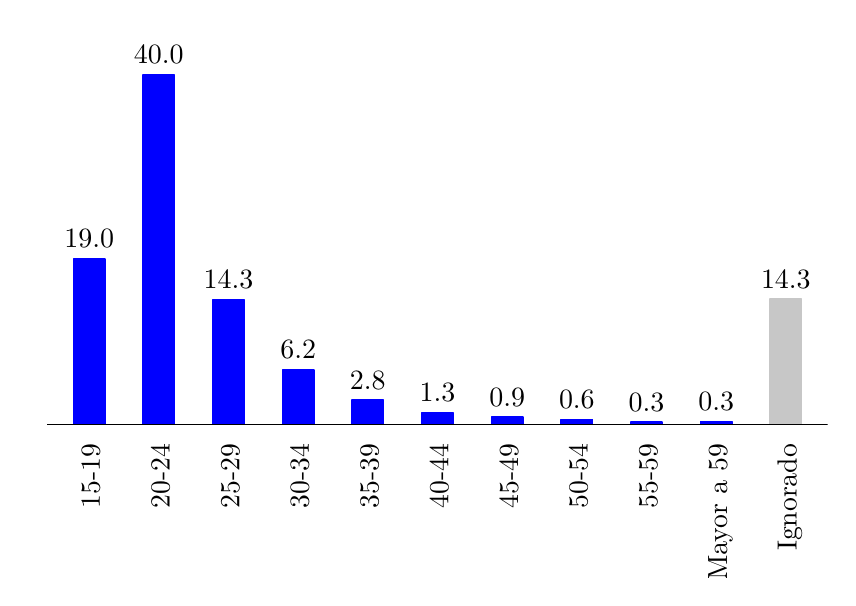
\begin{tikzpicture}[x=1pt,y=1pt]  % Created by tikzDevice version 0.7.0 on 2015-08-28 16:20:10
% !TEX encoding = UTF-8 Unicode
\definecolor[named]{fillColor}{rgb}{1.00,1.00,1.00}
\path[use as bounding box,fill=fillColor,fill opacity=0.00] (0,0) rectangle (289.08,198.74);
\begin{scope}
\path[clip] (  0.00,  0.00) rectangle (289.08,198.74);
\definecolor[named]{drawColor}{rgb}{1.00,1.00,1.00}

\path[draw=drawColor,line width= 0.6pt,line join=round,line cap=round] (  0.00,  0.00) rectangle (289.08,198.74);
\end{scope}
\begin{scope}
\path[clip] (  0.00,  0.00) rectangle (289.08,198.74);

\path[] (  7.11, 55.39) rectangle (289.08,181.67);

\path[] ( 22.22, 55.39) --
	( 22.22,181.67);

\path[] ( 47.39, 55.39) --
	( 47.39,181.67);

\path[] ( 72.57, 55.39) --
	( 72.57,181.67);

\path[] ( 97.75, 55.39) --
	( 97.75,181.67);

\path[] (122.92, 55.39) --
	(122.92,181.67);

\path[] (148.10, 55.39) --
	(148.10,181.67);

\path[] (173.27, 55.39) --
	(173.27,181.67);

\path[] (198.45, 55.39) --
	(198.45,181.67);

\path[] (223.62, 55.39) --
	(223.62,181.67);

\path[] (248.80, 55.39) --
	(248.80,181.67);

\path[] (273.97, 55.39) --
	(273.97,181.67);
\definecolor[named]{drawColor}{rgb}{0.00,0.00,1.00}
\definecolor[named]{fillColor}{rgb}{0.00,0.00,1.00}

\path[draw=drawColor,line width= 0.6pt,line join=round,fill=fillColor] ( 16.55, 55.39) rectangle ( 27.88,115.21);

\path[draw=drawColor,line width= 0.6pt,line join=round,fill=fillColor] ( 41.73, 55.39) rectangle ( 53.06,181.67);

\path[draw=drawColor,line width= 0.6pt,line join=round,fill=fillColor] ( 66.91, 55.39) rectangle ( 78.23,100.50);

\path[draw=drawColor,line width= 0.6pt,line join=round,fill=fillColor] ( 92.08, 55.39) rectangle (103.41, 75.09);

\path[draw=drawColor,line width= 0.6pt,line join=round,fill=fillColor] (117.26, 55.39) rectangle (128.59, 64.15);

\path[draw=drawColor,line width= 0.6pt,line join=round,fill=fillColor] (142.43, 55.39) rectangle (153.76, 59.63);

\path[draw=drawColor,line width= 0.6pt,line join=round,fill=fillColor] (167.61, 55.39) rectangle (178.94, 58.08);

\path[draw=drawColor,line width= 0.6pt,line join=round,fill=fillColor] (192.78, 55.39) rectangle (204.11, 57.21);

\path[draw=drawColor,line width= 0.6pt,line join=round,fill=fillColor] (217.96, 55.39) rectangle (229.29, 56.24);

\path[draw=drawColor,line width= 0.6pt,line join=round,fill=fillColor] (243.13, 55.39) rectangle (254.46, 56.41);
\definecolor[named]{drawColor}{rgb}{0.78,0.78,0.78}
\definecolor[named]{fillColor}{rgb}{0.78,0.78,0.78}

\path[draw=drawColor,line width= 0.6pt,line join=round,fill=fillColor] (268.31, 55.39) rectangle (279.64,100.63);
\definecolor[named]{drawColor}{rgb}{0.00,0.00,0.00}
\definecolor[named]{fillColor}{rgb}{0.00,0.00,0.00}

\path[draw=drawColor,line width= 0.1pt,line join=round,fill=fillColor] (  7.11, 55.39) -- (289.08, 55.39);

\node[text=drawColor,anchor=base,inner sep=0pt, outer sep=0pt, scale=  1.01] at ( 22.22,119.17) {19.0};

\node[text=drawColor,anchor=base,inner sep=0pt, outer sep=0pt, scale=  1.01] at ( 47.39,185.63) {40.0};

\node[text=drawColor,anchor=base,inner sep=0pt, outer sep=0pt, scale=  1.01] at ( 72.57,104.45) {14.3};

\node[text=drawColor,anchor=base,inner sep=0pt, outer sep=0pt, scale=  1.01] at ( 97.75, 79.04) {6.2};

\node[text=drawColor,anchor=base,inner sep=0pt, outer sep=0pt, scale=  1.01] at (122.92, 68.10) {2.8};

\node[text=drawColor,anchor=base,inner sep=0pt, outer sep=0pt, scale=  1.01] at (148.10, 63.59) {1.3};

\node[text=drawColor,anchor=base,inner sep=0pt, outer sep=0pt, scale=  1.01] at (173.27, 62.03) {0.9};

\node[text=drawColor,anchor=base,inner sep=0pt, outer sep=0pt, scale=  1.01] at (198.45, 61.17) {0.6};

\node[text=drawColor,anchor=base,inner sep=0pt, outer sep=0pt, scale=  1.01] at (223.62, 60.20) {0.3};

\node[text=drawColor,anchor=base,inner sep=0pt, outer sep=0pt, scale=  1.01] at (248.80, 60.37) {0.3};

\node[text=drawColor,anchor=base,inner sep=0pt, outer sep=0pt, scale=  1.01] at (273.97,104.59) {14.3};
\end{scope}
\begin{scope}
\path[clip] (  0.00,  0.00) rectangle (289.08,198.74);

\path[] (  7.11, 55.39) --
	(  7.11,181.67);
\end{scope}
\begin{scope}
\path[clip] (  0.00,  0.00) rectangle (289.08,198.74);

\path[] (  7.11, 55.39) --
	(289.08, 55.39);
\end{scope}
\begin{scope}
\path[clip] (  0.00,  0.00) rectangle (289.08,198.74);

\path[] ( 22.22, 51.12) --
	( 22.22, 55.39);

\path[] ( 47.39, 51.12) --
	( 47.39, 55.39);

\path[] ( 72.57, 51.12) --
	( 72.57, 55.39);

\path[] ( 97.75, 51.12) --
	( 97.75, 55.39);

\path[] (122.92, 51.12) --
	(122.92, 55.39);

\path[] (148.10, 51.12) --
	(148.10, 55.39);

\path[] (173.27, 51.12) --
	(173.27, 55.39);

\path[] (198.45, 51.12) --
	(198.45, 55.39);

\path[] (223.62, 51.12) --
	(223.62, 55.39);

\path[] (248.80, 51.12) --
	(248.80, 55.39);

\path[] (273.97, 51.12) --
	(273.97, 55.39);
\end{scope}
\begin{scope}
\path[clip] (  0.00,  0.00) rectangle (289.08,198.74);
\definecolor[named]{drawColor}{rgb}{0.00,0.00,0.00}

\node[text=drawColor,rotate= 90.00,anchor=base east,inner sep=0pt, outer sep=0pt, scale=  1.00] at ( 26.13, 48.28) {15-19};

\node[text=drawColor,rotate= 90.00,anchor=base east,inner sep=0pt, outer sep=0pt, scale=  1.00] at ( 51.30, 48.28) {20-24};

\node[text=drawColor,rotate= 90.00,anchor=base east,inner sep=0pt, outer sep=0pt, scale=  1.00] at ( 76.48, 48.28) {25-29};

\node[text=drawColor,rotate= 90.00,anchor=base east,inner sep=0pt, outer sep=0pt, scale=  1.00] at (101.65, 48.28) {30-34};

\node[text=drawColor,rotate= 90.00,anchor=base east,inner sep=0pt, outer sep=0pt, scale=  1.00] at (126.83, 48.28) {35-39};

\node[text=drawColor,rotate= 90.00,anchor=base east,inner sep=0pt, outer sep=0pt, scale=  1.00] at (152.01, 48.28) {40-44};

\node[text=drawColor,rotate= 90.00,anchor=base east,inner sep=0pt, outer sep=0pt, scale=  1.00] at (177.18, 48.28) {45-49};

\node[text=drawColor,rotate= 90.00,anchor=base east,inner sep=0pt, outer sep=0pt, scale=  1.00] at (202.36, 48.28) {50-54};

\node[text=drawColor,rotate= 90.00,anchor=base east,inner sep=0pt, outer sep=0pt, scale=  1.00] at (227.53, 48.28) {55-59};

\node[text=drawColor,rotate= 90.00,anchor=base east,inner sep=0pt, outer sep=0pt, scale=  1.00] at (252.71, 48.28) {Mayor a  59};

\node[text=drawColor,rotate= 90.00,anchor=base east,inner sep=0pt, outer sep=0pt, scale=  1.00] at (277.88, 48.28) {Ignorado};
\end{scope}
  \end{tikzpicture}}{Instituto Nacional de Estadística, con datos del Ministerio de Educación}

\cajota{Cobertura bruta en los departamentos}{Los departamentos con las mayores tasas brutas de cobertura en primaria  fueron: Sololá 83.0\%, Totonicapán 80.8\% y Petén 79.3\%.
	
	 Los departamentos con las más bajas tasas brutas de cobertura en primaria en el 2014, fueron: Zacapa 112.0\%, El Progreso 108.1\% y Santa Rosa 107.8\%. El departamento de Guatemala presentó una tasa de 104.6\%.}{Tasa bruta de cobertura del ciclo de educación primaria}{Por departamento, año 2014, en porcentaje}{\includegraphics[width=52\cuadri]{graficas/primaria/1_10.pdf}}{Instituto Nacional de Estadística, con datos del Ministerio de Educación}

\cajita{Cobertura neta}{La tasa neta de cobertura en primaria presentó el año 2009 el 98.7\% y en el año 2014 fue de 82.3\%, presentando un decrecimiento del 16.4 puntos porcentuales.}{Tasa neta de cobertura del ciclo de educación primaria}{República de Guatemala, serie histórica, en porcentaje}{\ \\[0mm]\begin{tikzpicture}[x=1pt,y=1pt]  % Created by tikzDevice version 0.7.0 on 2015-08-28 13:06:39
% !TEX encoding = UTF-8 Unicode
\definecolor[named]{fillColor}{rgb}{1.00,1.00,1.00}
\path[use as bounding box,fill=fillColor,fill opacity=0.00] (0,0) rectangle (289.08,198.74);
\begin{scope}
\path[clip] (  0.00,  0.00) rectangle (289.08,198.74);
\definecolor[named]{drawColor}{rgb}{1.00,1.00,1.00}

\path[draw=drawColor,line width= 0.6pt,line join=round,line cap=round] (  0.00,  0.00) rectangle (289.08,198.74);
\end{scope}
\begin{scope}
\path[clip] (  0.00,  0.00) rectangle (289.08,198.74);

\path[] (  6.02, 17.78) rectangle (280.54,191.48);

\path[] (  6.02, 46.07) --
	(280.54, 46.07);

\path[] (  6.02, 86.88) --
	(280.54, 86.88);

\path[] (  6.02,127.68) --
	(280.54,127.68);

\path[] (  6.02,168.49) --
	(280.54,168.49);

\path[] (  6.02, 25.67) --
	(280.54, 25.67);

\path[] (  6.02, 66.48) --
	(280.54, 66.48);

\path[] (  6.02,107.28) --
	(280.54,107.28);

\path[] (  6.02,148.09) --
	(280.54,148.09);

\path[] (  6.02,188.89) --
	(280.54,188.89);

\path[] ( 37.70, 17.78) --
	( 37.70,191.48);

\path[] ( 90.49, 17.78) --
	( 90.49,191.48);

\path[] (143.28, 17.78) --
	(143.28,191.48);

\path[] (196.08, 17.78) --
	(196.08,191.48);

\path[] (248.87, 17.78) --
	(248.87,191.48);
\definecolor[named]{drawColor}{rgb}{0.00,0.00,1.00}

\path[draw=drawColor,line width= 1.7pt,line join=round] ( 37.70,183.59) --
	( 90.49,171.75) --
	(143.28,159.51) --
	(196.08,144.41) --
	(248.87,129.32);
\definecolor[named]{drawColor}{rgb}{0.00,0.00,0.00}

\node[text=drawColor,anchor=base,inner sep=0pt, outer sep=0pt, scale=  1.01] at ( 37.70,187.54) {98.7};

\node[text=drawColor,anchor=base west,inner sep=0pt, outer sep=0pt, scale=  1.01] at ( 90.49,175.71) {95.8};

\node[text=drawColor,anchor=base west,inner sep=0pt, outer sep=0pt, scale=  1.01] at (143.28,163.47) {92.8};

\node[text=drawColor,anchor=base west,inner sep=0pt, outer sep=0pt, scale=  1.01] at (196.08,148.37) {89.1};

\node[text=drawColor,anchor=base,inner sep=0pt, outer sep=0pt, scale=  1.01] at (248.87,117.45) {85.4};
\definecolor[named]{fillColor}{rgb}{0.00,0.00,0.00}

\path[draw=drawColor,line width= 0.1pt,line join=round,fill=fillColor] (  6.02, 25.67) -- (280.54, 25.67);
\end{scope}
\begin{scope}
\path[clip] (  0.00,  0.00) rectangle (289.08,198.74);

\path[] (  6.02, 17.78) --
	(  6.02,191.48);
\end{scope}
\begin{scope}
\path[clip] (  0.00,  0.00) rectangle (289.08,198.74);

\path[] (  1.76, 25.67) --
	(  6.02, 25.67);

\path[] (  1.76, 66.48) --
	(  6.02, 66.48);

\path[] (  1.76,107.28) --
	(  6.02,107.28);

\path[] (  1.76,148.09) --
	(  6.02,148.09);

\path[] (  1.76,188.89) --
	(  6.02,188.89);
\end{scope}
\begin{scope}
\path[clip] (  0.00,  0.00) rectangle (289.08,198.74);

\path[] (  6.02, 17.78) --
	(280.54, 17.78);
\end{scope}
\begin{scope}
\path[clip] (  0.00,  0.00) rectangle (289.08,198.74);

\path[] ( 37.70, 13.51) --
	( 37.70, 17.78);

\path[] ( 90.49, 13.51) --
	( 90.49, 17.78);

\path[] (143.28, 13.51) --
	(143.28, 17.78);

\path[] (196.08, 13.51) --
	(196.08, 17.78);

\path[] (248.87, 13.51) --
	(248.87, 17.78);
\end{scope}
\begin{scope}
\path[clip] (  0.00,  0.00) rectangle (289.08,198.74);
\definecolor[named]{drawColor}{rgb}{0.00,0.00,0.00}

\node[text=drawColor,anchor=base,inner sep=0pt, outer sep=0pt, scale=  1.00] at ( 37.70,  2.85) {2009};

\node[text=drawColor,anchor=base,inner sep=0pt, outer sep=0pt, scale=  1.00] at ( 90.49,  2.85) {2010};

\node[text=drawColor,anchor=base,inner sep=0pt, outer sep=0pt, scale=  1.00] at (143.28,  2.85) {2011};

\node[text=drawColor,anchor=base,inner sep=0pt, outer sep=0pt, scale=  1.00] at (196.08,  2.85) {2012};

\node[text=drawColor,anchor=base,inner sep=0pt, outer sep=0pt, scale=  1.00] at (248.87,  2.85) {2014};
\end{scope}
  \end{tikzpicture}}{Instituto Nacional de Estadística, con datos del Ministerio de Educación}

\cajita{Cobertura neta por sexo}{La tasa neta de cobertura en primaria por sexo, representa el 82.7\% para hombres y 81.9\% para las mujeres.}{Tasa neta de cobertura del ciclo de educación primaria, por sexo}{República de Guatemala, año 2014, en porcentaje}{\ \\[0mm]\begin{tikzpicture}[x=1pt,y=1pt]  % Created by tikzDevice version 0.7.0 on 2015-09-01 14:24:00
% !TEX encoding = UTF-8 Unicode
\definecolor[named]{fillColor}{rgb}{1.00,1.00,1.00}
\path[use as bounding box,fill=fillColor,fill opacity=0.00] (0,0) rectangle (289.08,198.74);
\begin{scope}
\path[clip] (  0.00,  0.00) rectangle (289.08,198.74);
\definecolor[named]{drawColor}{rgb}{1.00,1.00,1.00}

\path[draw=drawColor,line width= 0.6pt,line join=round,line cap=round] (  0.00,  0.00) rectangle (289.08,198.74);
\end{scope}
\begin{scope}
\path[clip] (  0.00,  0.00) rectangle (289.08,198.74);

\path[] (  1.64, 17.78) rectangle (280.54,191.48);

\path[] (  1.64, 47.21) --
	(280.54, 47.21);

\path[] (  1.64, 90.30) --
	(280.54, 90.30);

\path[] (  1.64,133.39) --
	(280.54,133.39);

\path[] (  1.64,176.48) --
	(280.54,176.48);

\path[] (  1.64, 25.67) --
	(280.54, 25.67);

\path[] (  1.64, 68.76) --
	(280.54, 68.76);

\path[] (  1.64,111.85) --
	(280.54,111.85);

\path[] (  1.64,154.93) --
	(280.54,154.93);

\path[] ( 33.83, 17.78) --
	( 33.83,191.48);

\path[] ( 87.46, 17.78) --
	( 87.46,191.48);

\path[] (141.09, 17.78) --
	(141.09,191.48);

\path[] (194.73, 17.78) --
	(194.73,191.48);

\path[] (248.36, 17.78) --
	(248.36,191.48);
\definecolor[named]{drawColor}{rgb}{0.00,0.00,1.00}

\path[draw=drawColor,line width= 1.7pt,line join=round] ( 33.83, 96.77) --
	( 87.46,123.48) --
	(141.09,133.39) --
	(194.73,167.64) --
	(248.36,183.59);
\definecolor[named]{drawColor}{rgb}{0.00,0.00,0.00}

\node[text=drawColor,anchor=base,inner sep=0pt, outer sep=0pt, scale=  1.01] at ( 33.83, 84.90) {53.0};

\node[text=drawColor,anchor=base east,inner sep=0pt, outer sep=0pt, scale=  1.01] at ( 84.34,123.48) {65.4};

\node[text=drawColor,anchor=base east,inner sep=0pt, outer sep=0pt, scale=  1.01] at (137.98,133.39) {70.0};

\node[text=drawColor,anchor=base east,inner sep=0pt, outer sep=0pt, scale=  1.01] at (191.61,167.64) {85.9};

\node[text=drawColor,anchor=base,inner sep=0pt, outer sep=0pt, scale=  1.01] at (248.36,187.54) {93.3};
\definecolor[named]{fillColor}{rgb}{0.00,0.00,0.00}

\path[draw=drawColor,line width= 0.1pt,line join=round,fill=fillColor] (  1.64, 25.67) -- (280.54, 25.67);
\end{scope}
\begin{scope}
\path[clip] (  0.00,  0.00) rectangle (289.08,198.74);

\path[] (  1.64, 17.78) --
	(  1.64,191.48);
\end{scope}
\begin{scope}
\path[clip] (  0.00,  0.00) rectangle (289.08,198.74);

\path[] (  0.00, 25.67) --
	(  1.64, 25.67);

\path[] (  0.00, 68.76) --
	(  1.64, 68.76);

\path[] (  0.00,111.85) --
	(  1.64,111.85);

\path[] (  0.00,154.93) --
	(  1.64,154.93);
\end{scope}
\begin{scope}
\path[clip] (  0.00,  0.00) rectangle (289.08,198.74);

\path[] (  1.64, 17.78) --
	(280.54, 17.78);
\end{scope}
\begin{scope}
\path[clip] (  0.00,  0.00) rectangle (289.08,198.74);

\path[] ( 33.83, 13.51) --
	( 33.83, 17.78);

\path[] ( 87.46, 13.51) --
	( 87.46, 17.78);

\path[] (141.09, 13.51) --
	(141.09, 17.78);

\path[] (194.73, 13.51) --
	(194.73, 17.78);

\path[] (248.36, 13.51) --
	(248.36, 17.78);
\end{scope}
\begin{scope}
\path[clip] (  0.00,  0.00) rectangle (289.08,198.74);
\definecolor[named]{drawColor}{rgb}{0.00,0.00,0.00}

\node[text=drawColor,anchor=base,inner sep=0pt, outer sep=0pt, scale=  1.00] at ( 33.83,  2.85) {1987};

\node[text=drawColor,anchor=base,inner sep=0pt, outer sep=0pt, scale=  1.00] at ( 87.46,  2.85) {1995};

\node[text=drawColor,anchor=base,inner sep=0pt, outer sep=0pt, scale=  1.00] at (141.09,  2.85) {1998/99};

\node[text=drawColor,anchor=base,inner sep=0pt, outer sep=0pt, scale=  1.00] at (194.73,  2.85) {2002};

\node[text=drawColor,anchor=base,inner sep=0pt, outer sep=0pt, scale=  1.00] at (248.36,  2.85) {2008/09};
\end{scope}
  \end{tikzpicture}}{Instituto Nacional de Estadística, con datos del Ministerio de Educación}

\cajota{Cobertura neta en los departamentos}{El mapa muestra en color celeste los departamentos con las menores tasas netas de cobertura en primaria, que fueron: Sololá 70.3\%, Totonicapán 67.2\% y Petén 62.8\%. 
	
	Los departamentos donde que tuvieron una alta tasa neta de cobertura en primaria fueron: Zacapa 92.4\%, Guatemala 92.1 y San Marcos 90.5\%. }{Tasa neta de cobertura del ciclo de educación primaria}{Por departamento, año 2014, en porcentaje}{\includegraphics[width=52\cuadri]{graficas/primaria/1_13.pdf}}{Instituto Nacional de Estadística, con datos del Ministerio de Educación}




\cajita{Repitencia}{La tasa de repitencia en primaria es la relación que existe entre el número de repitentes y el número de alumnos que en el año  estaban inscritos en el mismo grado.
	
	En el año 2009 fue del 11.5\% y en el 2014 fue de 9.1\%, presentando una disminución de 2.4 puntos porcentuales.}{Tasa de repitencia del ciclo de educación primaria}{República de Guatemala, serie histórica, en porcentaje}{\ \\[0mm]\begin{tikzpicture}[x=1pt,y=1pt]  % Created by tikzDevice version 0.9 on 2016-02-29 21:53:58
% !TEX encoding = UTF-8 Unicode
\definecolor{fillColor}{RGB}{255,255,255}
\path[use as bounding box,fill=fillColor,fill opacity=0.00] (0,0) rectangle (289.08,198.74);
\begin{scope}
\path[clip] (  0.00,  0.00) rectangle (289.08,198.74);

\path[] (  0.00,  0.00) rectangle (289.08,198.74);
\end{scope}
\begin{scope}
\path[clip] (  0.00,  0.00) rectangle (289.08,198.74);

\path[] ( -0.52, 15.61) rectangle (280.54,191.48);

\path[] (  0.00, 23.61) --
	(280.54, 23.61);

\path[] (  0.00, 69.95) --
	(280.54, 69.95);

\path[] (  0.00,116.29) --
	(280.54,116.29);

\path[] (  0.00,162.63) --
	(280.54,162.63);

\path[] (  0.00, 46.78) --
	(280.54, 46.78);

\path[] (  0.00, 93.12) --
	(280.54, 93.12);

\path[] (  0.00,139.46) --
	(280.54,139.46);

\path[] (  0.00,185.81) --
	(280.54,185.81);

\path[] ( 26.68, 15.61) --
	( 26.68,191.48);

\path[] ( 72.01, 15.61) --
	( 72.01,191.48);

\path[] (117.35, 15.61) --
	(117.35,191.48);

\path[] (162.68, 15.61) --
	(162.68,191.48);

\path[] (208.01, 15.61) --
	(208.01,191.48);

\path[] (253.34, 15.61) --
	(253.34,191.48);
\definecolor{drawColor}{RGB}{0,0,255}

\path[draw=drawColor,line width= 1.7pt,line join=round] ( 26.68,173.99) --
	( 72.01,183.49) --
	(117.35,160.78) --
	(162.68,181.87) --
	(208.01,143.87) --
	(253.34,118.38);
\definecolor{drawColor}{RGB}{0,0,0}

\node[text=drawColor,anchor=base,inner sep=0pt, outer sep=0pt, scale=  1.02] at ( 26.68,162.08) {11.5};

\node[text=drawColor,anchor=base,inner sep=0pt, outer sep=0pt, scale=  1.02] at ( 72.01,187.46) {11.9};

\node[text=drawColor,anchor=base,inner sep=0pt, outer sep=0pt, scale=  1.02] at (117.35,148.87) {10.9};

\node[text=drawColor,anchor=base,inner sep=0pt, outer sep=0pt, scale=  1.02] at (162.68,185.84) {11.8};

\node[text=drawColor,anchor=base west,inner sep=0pt, outer sep=0pt, scale=  1.02] at (208.01,147.84) {10.2};

\node[text=drawColor,anchor=base,inner sep=0pt, outer sep=0pt, scale=  1.02] at (253.34,106.46) {9.1};

\path[draw=drawColor,line width= 0.1pt,line join=round] (  0.00, 23.61) -- (280.54, 23.61);

\path[] ( -0.52, 15.61) rectangle (280.54,191.48);
\end{scope}
\begin{scope}
\path[clip] (  0.00,  0.00) rectangle (289.08,198.74);

\path[] (  0.00, 15.61) --
	(280.54, 15.61);
\end{scope}
\begin{scope}
\path[clip] (  0.00,  0.00) rectangle (289.08,198.74);

\path[] ( 26.68, 12.86) --
	( 26.68, 15.61);

\path[] ( 72.01, 12.86) --
	( 72.01, 15.61);

\path[] (117.35, 12.86) --
	(117.35, 15.61);

\path[] (162.68, 12.86) --
	(162.68, 15.61);

\path[] (208.01, 12.86) --
	(208.01, 15.61);

\path[] (253.34, 12.86) --
	(253.34, 15.61);
\end{scope}
\begin{scope}
\path[clip] (  0.00,  0.00) rectangle (289.08,198.74);
\definecolor{drawColor}{RGB}{0,0,0}

\node[text=drawColor,anchor=base,inner sep=0pt, outer sep=0pt, scale=  1.00] at ( 26.68,  2.85) {2009};

\node[text=drawColor,anchor=base,inner sep=0pt, outer sep=0pt, scale=  1.00] at ( 72.01,  2.85) {2010};

\node[text=drawColor,anchor=base,inner sep=0pt, outer sep=0pt, scale=  1.00] at (117.35,  2.85) {2011};

\node[text=drawColor,anchor=base,inner sep=0pt, outer sep=0pt, scale=  1.00] at (162.68,  2.85) {2012};

\node[text=drawColor,anchor=base,inner sep=0pt, outer sep=0pt, scale=  1.00] at (208.01,  2.85) {2013};

\node[text=drawColor,anchor=base,inner sep=0pt, outer sep=0pt, scale=  1.00] at (253.34,  2.85) {2014};
\end{scope}
  \end{tikzpicture}}{Instituto Nacional de Estadística, con datos del Ministerio de Educación}

\cajita{Repitencia por sexo}{La tasa de repitencia en primaria por sexo, representó el 10.1\% para hombres y 8.0\% para las mujeres.}{Tasa de repitencia del ciclo de educación primaria, por sexo}{República de Guatemala, año 2014, en porcentaje}{\ \\[0mm]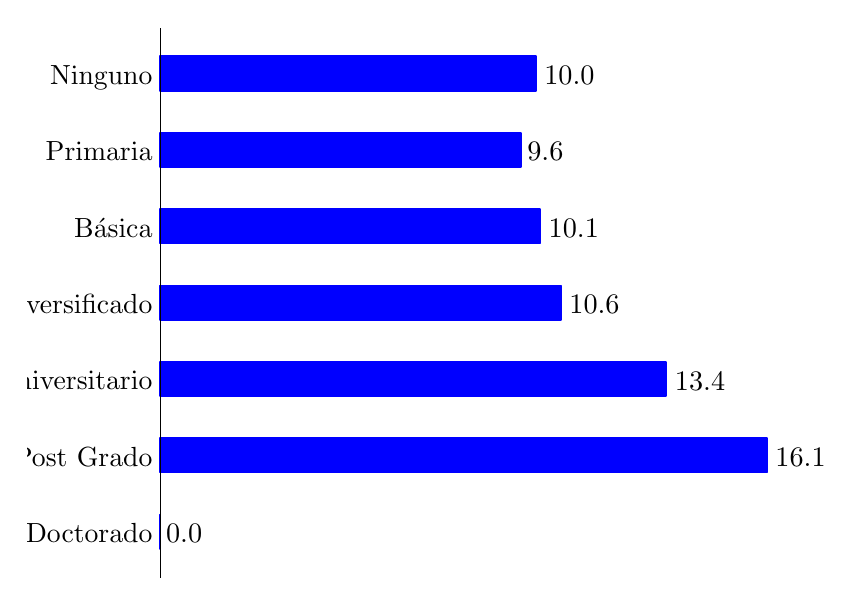
\begin{tikzpicture}[x=1pt,y=1pt]  % Created by tikzDevice version 0.10.1 on 2016-02-29 14:42:48
% !TEX encoding = UTF-8 Unicode
\definecolor{fillColor}{RGB}{255,255,255}
\path[use as bounding box,fill=fillColor,fill opacity=0.00] (0,0) rectangle (289.08,198.74);
\begin{scope}
\path[clip] (  0.00,  0.00) rectangle (289.08,198.74);

\path[] (  0.00,  0.00) rectangle (289.08,198.74);
\end{scope}
\begin{scope}
\path[clip] (  0.00,  0.00) rectangle (289.08,198.74);

\path[] ( 47.80,  0.00) rectangle (267.09,198.74);

\path[] ( 47.80, 16.56) --
	(267.09, 16.56);

\path[] ( 47.80, 44.16) --
	(267.09, 44.16);

\path[] ( 47.80, 71.77) --
	(267.09, 71.77);

\path[] ( 47.80, 99.37) --
	(267.09, 99.37);

\path[] ( 47.80,126.97) --
	(267.09,126.97);

\path[] ( 47.80,154.58) --
	(267.09,154.58);

\path[] ( 47.80,182.18) --
	(267.09,182.18);
\definecolor{drawColor}{RGB}{0,0,255}
\definecolor{fillColor}{RGB}{0,0,255}

\path[draw=drawColor,line width= 0.6pt,line join=round,fill=fillColor] ( 47.80, 10.35) rectangle ( 47.80, 22.77);

\path[draw=drawColor,line width= 0.6pt,line join=round,fill=fillColor] ( 47.80, 37.95) rectangle (267.09, 50.38);

\path[draw=drawColor,line width= 0.6pt,line join=round,fill=fillColor] ( 47.80, 65.56) rectangle (230.77, 77.98);

\path[draw=drawColor,line width= 0.6pt,line join=round,fill=fillColor] ( 47.80, 93.16) rectangle (192.63,105.58);

\path[draw=drawColor,line width= 0.6pt,line join=round,fill=fillColor] ( 47.80,120.76) rectangle (185.14,133.19);

\path[draw=drawColor,line width= 0.6pt,line join=round,fill=fillColor] ( 47.80,148.37) rectangle (178.32,160.79);

\path[draw=drawColor,line width= 0.6pt,line join=round,fill=fillColor] ( 47.80,175.97) rectangle (183.58,188.39);
\definecolor{drawColor}{RGB}{0,0,0}

\path[draw=drawColor,line width= 0.1pt,line join=round] ( 47.80,  0.00) -- ( 47.80,198.74);

\node[text=drawColor,anchor=base west,inner sep=0pt, outer sep=0pt, scale=  1.02] at ( 50.03, 12.59) {0.0};

\node[text=drawColor,anchor=base west,inner sep=0pt, outer sep=0pt, scale=  1.02] at (270.21, 40.19) {16.1};

\node[text=drawColor,anchor=base west,inner sep=0pt, outer sep=0pt, scale=  1.02] at (233.89, 67.80) {13.4};

\node[text=drawColor,anchor=base west,inner sep=0pt, outer sep=0pt, scale=  1.02] at (195.76, 95.40) {10.6};

\node[text=drawColor,anchor=base west,inner sep=0pt, outer sep=0pt, scale=  1.02] at (188.27,123.00) {10.1};

\node[text=drawColor,anchor=base west,inner sep=0pt, outer sep=0pt, scale=  1.02] at (180.56,150.61) {9.6};

\node[text=drawColor,anchor=base west,inner sep=0pt, outer sep=0pt, scale=  1.02] at (186.71,178.21) {10.0};

\path[] ( 47.80,  0.00) rectangle (267.09,198.74);
\end{scope}
\begin{scope}
\path[clip] (  0.00,  0.00) rectangle (289.08,198.74);

\path[] ( 47.80,  0.00) --
	( 47.80,198.74);
\end{scope}
\begin{scope}
\path[clip] (  0.00,  0.00) rectangle (289.08,198.74);
\definecolor{drawColor}{RGB}{0,0,0}

\node[text=drawColor,anchor=base east,inner sep=0pt, outer sep=0pt, scale=  1.00] at ( 45.05, 12.65) {Doctorado};

\node[text=drawColor,anchor=base east,inner sep=0pt, outer sep=0pt, scale=  1.00] at ( 45.05, 40.26) {Post Grado};

\node[text=drawColor,anchor=base east,inner sep=0pt, outer sep=0pt, scale=  1.00] at ( 45.05, 67.86) {Universitario};

\node[text=drawColor,anchor=base east,inner sep=0pt, outer sep=0pt, scale=  1.00] at ( 45.05, 95.46) {Diversificado};

\node[text=drawColor,anchor=base east,inner sep=0pt, outer sep=0pt, scale=  1.00] at ( 45.05,123.07) {Básica};

\node[text=drawColor,anchor=base east,inner sep=0pt, outer sep=0pt, scale=  1.00] at ( 45.05,150.67) {Primaria};

\node[text=drawColor,anchor=base east,inner sep=0pt, outer sep=0pt, scale=  1.00] at ( 45.05,178.27) {Ninguno};
\end{scope}
\begin{scope}
\path[clip] (  0.00,  0.00) rectangle (289.08,198.74);

\path[] ( 45.05, 16.56) --
	( 47.80, 16.56);

\path[] ( 45.05, 44.16) --
	( 47.80, 44.16);

\path[] ( 45.05, 71.77) --
	( 47.80, 71.77);

\path[] ( 45.05, 99.37) --
	( 47.80, 99.37);

\path[] ( 45.05,126.97) --
	( 47.80,126.97);

\path[] ( 45.05,154.58) --
	( 47.80,154.58);

\path[] ( 45.05,182.18) --
	( 47.80,182.18);
\end{scope}
  \end{tikzpicture}}{Instituto Nacional de Estadística, con datos del Ministerio de Educación}

\cajota{Repitencia en los departamentos}{El mapa muestra en color celeste los departamentos con las menores tasas de repitencia en primaria, que fueron: Jutiapa 6.5\%, Retalhuleu 6.3\% y Guatemala 4.0\%.  
	
	Los departamentos con las mayores tasas  de repitencia en primaria:  Alta Verapaz con 15.6\%, Jalapa 12.3\% y Zacapa 11.9\%.}{Tasa de repitencia del ciclo de educación primaria}{Por departamento, año 2014, en porcentaje}{\includegraphics[width=52\cuadri]{graficas/primaria/1_16.pdf}}{Instituto Nacional de Estadística, con datos del Ministerio de Educación}






\cajita{Sobre-edad}{La tasa de  sobre-edad , es la relación que existe entre la cantidad de alumnos inscritos en los diferentes grados de un nivel educativo, con dos o más años de atraso escolar por encima de la edad correspondiente al grado de estudio. 
	
	En el año 2009 fue del 51.7\% y en el año 2014 fue de 15.4\%, presentando una disminución de 36.3 puntos porcentuales.}{Tasa de sobre-edad del ciclo de educación primaria}{República de Guatemala, serie histórica, en porcentaje}{\ \\[0mm]\begin{tikzpicture}[x=1pt,y=1pt]  % Created by tikzDevice version 0.9 on 2016-02-29 21:54:02
% !TEX encoding = UTF-8 Unicode
\definecolor{fillColor}{RGB}{255,255,255}
\path[use as bounding box,fill=fillColor,fill opacity=0.00] (0,0) rectangle (289.08,198.74);
\begin{scope}
\path[clip] (  0.00,  0.00) rectangle (289.08,198.74);

\path[] (  0.00,  0.00) rectangle (289.08,198.74);
\end{scope}
\begin{scope}
\path[clip] (  0.00,  0.00) rectangle (289.08,198.74);

\path[] ( -0.52, 15.61) rectangle (280.54,191.48);

\path[] (  0.00, 39.07) --
	(280.54, 39.07);

\path[] (  0.00, 70.00) --
	(280.54, 70.00);

\path[] (  0.00,100.93) --
	(280.54,100.93);

\path[] (  0.00,131.86) --
	(280.54,131.86);

\path[] (  0.00,162.80) --
	(280.54,162.80);

\path[] (  0.00, 23.61) --
	(280.54, 23.61);

\path[] (  0.00, 54.54) --
	(280.54, 54.54);

\path[] (  0.00, 85.47) --
	(280.54, 85.47);

\path[] (  0.00,116.40) --
	(280.54,116.40);

\path[] (  0.00,147.33) --
	(280.54,147.33);

\path[] (  0.00,178.26) --
	(280.54,178.26);

\path[] ( 26.68, 15.61) --
	( 26.68,191.48);

\path[] ( 72.01, 15.61) --
	( 72.01,191.48);

\path[] (117.35, 15.61) --
	(117.35,191.48);

\path[] (162.68, 15.61) --
	(162.68,191.48);

\path[] (208.01, 15.61) --
	(208.01,191.48);

\path[] (253.34, 15.61) --
	(253.34,191.48);
\definecolor{drawColor}{RGB}{0,0,255}

\path[draw=drawColor,line width= 1.7pt,line join=round] ( 26.68,183.49) --
	( 72.01,105.73) --
	(117.35, 94.59) --
	(162.68, 90.97) --
	(208.01, 87.85) --
	(253.34, 71.09);
\definecolor{drawColor}{RGB}{0,0,0}

\node[text=drawColor,anchor=base,inner sep=0pt, outer sep=0pt, scale=  1.02] at ( 26.68,187.46) {51.7};

\node[text=drawColor,anchor=base west,inner sep=0pt, outer sep=0pt, scale=  1.02] at ( 72.01,109.70) {26.6};

\node[text=drawColor,anchor=base west,inner sep=0pt, outer sep=0pt, scale=  1.02] at (117.35, 98.56) {22.9};

\node[text=drawColor,anchor=base west,inner sep=0pt, outer sep=0pt, scale=  1.02] at (162.68, 94.95) {21.8};

\node[text=drawColor,anchor=base west,inner sep=0pt, outer sep=0pt, scale=  1.02] at (208.01, 91.82) {20.8};

\node[text=drawColor,anchor=base,inner sep=0pt, outer sep=0pt, scale=  1.02] at (253.34, 59.17) {15.3};

\path[draw=drawColor,line width= 0.1pt,line join=round] (  0.00, 23.61) -- (280.54, 23.61);

\path[] ( -0.52, 15.61) rectangle (280.54,191.48);
\end{scope}
\begin{scope}
\path[clip] (  0.00,  0.00) rectangle (289.08,198.74);

\path[] (  0.00, 15.61) --
	(280.54, 15.61);
\end{scope}
\begin{scope}
\path[clip] (  0.00,  0.00) rectangle (289.08,198.74);

\path[] ( 26.68, 12.86) --
	( 26.68, 15.61);

\path[] ( 72.01, 12.86) --
	( 72.01, 15.61);

\path[] (117.35, 12.86) --
	(117.35, 15.61);

\path[] (162.68, 12.86) --
	(162.68, 15.61);

\path[] (208.01, 12.86) --
	(208.01, 15.61);

\path[] (253.34, 12.86) --
	(253.34, 15.61);
\end{scope}
\begin{scope}
\path[clip] (  0.00,  0.00) rectangle (289.08,198.74);
\definecolor{drawColor}{RGB}{0,0,0}

\node[text=drawColor,anchor=base,inner sep=0pt, outer sep=0pt, scale=  1.00] at ( 26.68,  2.85) {2009};

\node[text=drawColor,anchor=base,inner sep=0pt, outer sep=0pt, scale=  1.00] at ( 72.01,  2.85) {2010};

\node[text=drawColor,anchor=base,inner sep=0pt, outer sep=0pt, scale=  1.00] at (117.35,  2.85) {2011};

\node[text=drawColor,anchor=base,inner sep=0pt, outer sep=0pt, scale=  1.00] at (162.68,  2.85) {2012};

\node[text=drawColor,anchor=base,inner sep=0pt, outer sep=0pt, scale=  1.00] at (208.01,  2.85) {2013};

\node[text=drawColor,anchor=base,inner sep=0pt, outer sep=0pt, scale=  1.00] at (253.34,  2.85) {2014};
\end{scope}
  \end{tikzpicture}}{Instituto Nacional de Estadística, con datos del Ministerio de Educación}

\cajita{Sobre-edad por sexo}{La tasa de  sobre-edad en primaria por sexo, representa el 16.9\% para hombres y 13.7\% para las mujeres.}{Tasa de sobre-edad del ciclo de educación primaria, por sexo}{República de Guatemala, año 2014, en porcentaje}{\ \\[0mm]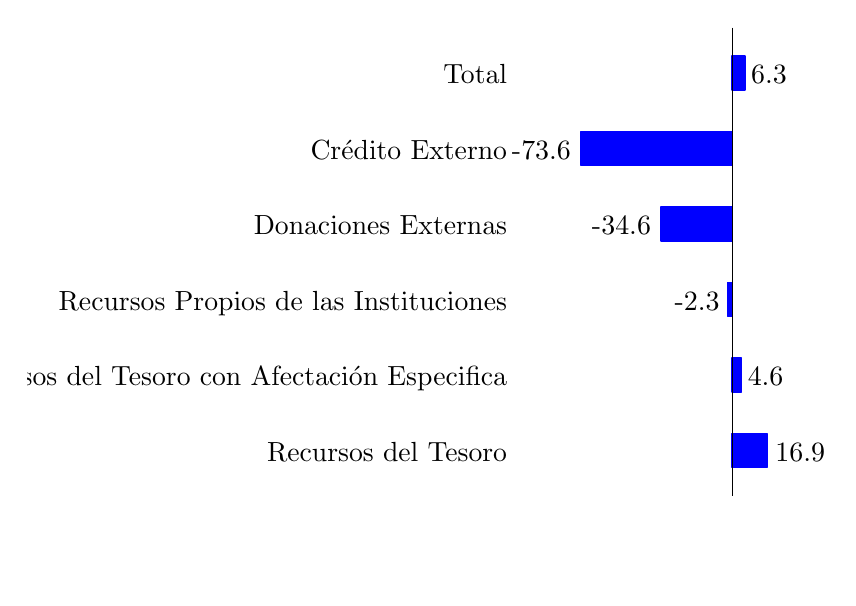
\begin{tikzpicture}[x=1pt,y=1pt]  % Created by tikzDevice version 0.7.0 on 2015-08-28 16:35:09
% !TEX encoding = UTF-8 Unicode
\definecolor[named]{fillColor}{rgb}{1.00,1.00,1.00}
\path[use as bounding box,fill=fillColor,fill opacity=0.00] (0,0) rectangle (289.08,198.74);
\begin{scope}
\path[clip] (  0.00,  0.00) rectangle (289.08,198.74);
\definecolor[named]{drawColor}{rgb}{1.00,1.00,1.00}

\path[draw=drawColor,line width= 0.6pt,line join=round,line cap=round] (  0.00,  0.00) rectangle (289.08,198.74);
\end{scope}
\begin{scope}
\path[clip] (  0.00,  0.00) rectangle (289.08,198.74);

\path[] (199.99, 29.60) rectangle (267.09,198.74);

\path[] (199.99, 45.97) --
	(267.09, 45.97);

\path[] (199.99, 73.25) --
	(267.09, 73.25);

\path[] (199.99,100.53) --
	(267.09,100.53);

\path[] (199.99,127.81) --
	(267.09,127.81);

\path[] (199.99,155.09) --
	(267.09,155.09);

\path[] (199.99,182.37) --
	(267.09,182.37);
\definecolor[named]{drawColor}{rgb}{0.00,0.00,1.00}
\definecolor[named]{fillColor}{rgb}{0.00,0.00,1.00}

\path[draw=drawColor,line width= 0.6pt,line join=round,fill=fillColor] (254.56, 39.83) rectangle (267.09, 52.11);

\path[draw=drawColor,line width= 0.6pt,line join=round,fill=fillColor] (254.56, 67.11) rectangle (257.97, 79.39);

\path[draw=drawColor,line width= 0.6pt,line join=round,fill=fillColor] (252.85, 94.39) rectangle (254.56,106.67);

\path[draw=drawColor,line width= 0.6pt,line join=round,fill=fillColor] (228.90,121.67) rectangle (254.56,133.95);

\path[draw=drawColor,line width= 0.6pt,line join=round,fill=fillColor] (199.99,148.95) rectangle (254.56,161.23);

\path[draw=drawColor,line width= 0.6pt,line join=round,fill=fillColor] (254.56,176.24) rectangle (259.23,188.51);
\definecolor[named]{drawColor}{rgb}{0.00,0.00,0.00}
\definecolor[named]{fillColor}{rgb}{0.00,0.00,0.00}

\path[draw=drawColor,line width= 0.1pt,line join=round,fill=fillColor] (254.56, 29.60) -- (254.56,198.74);

\node[text=drawColor,anchor=base west,inner sep=0pt, outer sep=0pt, scale=  1.01] at (270.20, 42.01) {16.9};

\node[text=drawColor,anchor=base west,inner sep=0pt, outer sep=0pt, scale=  1.01] at (260.20, 69.29) {4.6};

\node[text=drawColor,anchor=base east,inner sep=0pt, outer sep=0pt, scale=  1.01] at (250.06, 96.57) {-2.3};

\node[text=drawColor,anchor=base east,inner sep=0pt, outer sep=0pt, scale=  1.01] at (225.23,123.86) {-34.6};

\node[text=drawColor,anchor=base east,inner sep=0pt, outer sep=0pt, scale=  1.01] at (196.31,151.14) {-73.6};

\node[text=drawColor,anchor=base west,inner sep=0pt, outer sep=0pt, scale=  1.01] at (261.46,178.42) {6.3};
\end{scope}
\begin{scope}
\path[clip] (  0.00,  0.00) rectangle (289.08,198.74);

\path[] (199.99, 29.60) --
	(199.99,198.74);
\end{scope}
\begin{scope}
\path[clip] (  0.00,  0.00) rectangle (289.08,198.74);
\definecolor[named]{drawColor}{rgb}{0.00,0.00,0.00}

\node[text=drawColor,anchor=base east,inner sep=0pt, outer sep=0pt, scale=  1.00] at (173.23, 42.06) {Recursos del Tesoro};

\node[text=drawColor,anchor=base east,inner sep=0pt, outer sep=0pt, scale=  1.00] at (173.23, 69.34) {Recursos del Tesoro con Afectaci\'on Especifica};

\node[text=drawColor,anchor=base east,inner sep=0pt, outer sep=0pt, scale=  1.00] at (173.23, 96.62) {Recursos Propios de las Instituciones};

\node[text=drawColor,anchor=base east,inner sep=0pt, outer sep=0pt, scale=  1.00] at (173.23,123.90) {Donaciones Externas};

\node[text=drawColor,anchor=base east,inner sep=0pt, outer sep=0pt, scale=  1.00] at (173.23,151.18) {Cr\'edito Externo};

\node[text=drawColor,anchor=base east,inner sep=0pt, outer sep=0pt, scale=  1.00] at (173.23,178.47) {Total};
\end{scope}
\begin{scope}
\path[clip] (  0.00,  0.00) rectangle (289.08,198.74);

\path[] (173.23, 45.97) --
	(177.50, 45.97);

\path[] (173.23, 73.25) --
	(177.50, 73.25);

\path[] (173.23,100.53) --
	(177.50,100.53);

\path[] (173.23,127.81) --
	(177.50,127.81);

\path[] (173.23,155.09) --
	(177.50,155.09);

\path[] (173.23,182.37) --
	(177.50,182.37);
\end{scope}
\begin{scope}
\path[clip] (  0.00,  0.00) rectangle (289.08,198.74);

\path[] (199.99, 29.60) --
	(267.09, 29.60);
\end{scope}
  \end{tikzpicture}}{Instituto Nacional de Estadística, con datos del Ministerio de Educación}

\cajota{Sobre-edad en los departamentos}{El mapa muestra en color celeste los departamentos con las menores tasas de sobre-edad en primaria en el 2013, que fueron: Chimaltenango 10.9\%, Sacatepéquez 9.1\% y Guatemala 8.4\%.
	
	 Los departamentos con las mayores tasas  de sobre-edad en primaria: Petén 23.2\%, Alta Verapaz 21.5\% y Quiché 19.8\%.}{Tasa de sobre-edad del ciclo de educación primaria}{Por departamento, año 2014, en porcentaje}{\includegraphics[width=52\cuadri]{graficas/primaria/1_19.pdf}}{Instituto Nacional de Estadística, con datos del Ministerio de Educación}





\cajita{Deserción}{La tasa de deserción en primaria , se refiere a la cantidad de alumnos que no concluyen el ciclo lectivo. 
	
	En el año 2009 fue de 5.5\% y en el año 2013 fue de 3.6\%, presentando una disminución en 2 puntos porcentuales.}{Tasa de deserción del ciclo de educación primaria}{República de Guatemala, serie histórica, en porcentaje}{\ \\[0mm]\begin{tikzpicture}[x=1pt,y=1pt]  % Created by tikzDevice version 0.9 on 2016-02-29 21:54:07
% !TEX encoding = UTF-8 Unicode
\definecolor{fillColor}{RGB}{255,255,255}
\path[use as bounding box,fill=fillColor,fill opacity=0.00] (0,0) rectangle (289.08,198.74);
\begin{scope}
\path[clip] (  0.00,  0.00) rectangle (289.08,198.74);

\path[] (  0.00,  0.00) rectangle (289.08,198.74);
\end{scope}
\begin{scope}
\path[clip] (  0.00,  0.00) rectangle (289.08,198.74);

\path[] ( -4.90, 15.61) rectangle (280.54,191.48);

\path[] (  0.00, 50.30) --
	(280.54, 50.30);

\path[] (  0.00,103.68) --
	(280.54,103.68);

\path[] (  0.00,157.06) --
	(280.54,157.06);

\path[] (  0.00, 23.61) --
	(280.54, 23.61);

\path[] (  0.00, 76.99) --
	(280.54, 76.99);

\path[] (  0.00,130.37) --
	(280.54,130.37);

\path[] (  0.00,183.76) --
	(280.54,183.76);

\path[] ( 22.73, 15.61) --
	( 22.73,191.48);

\path[] ( 68.76, 15.61) --
	( 68.76,191.48);

\path[] (114.80, 15.61) --
	(114.80,191.48);

\path[] (160.84, 15.61) --
	(160.84,191.48);

\path[] (206.88, 15.61) --
	(206.88,191.48);

\path[] (252.92, 15.61) --
	(252.92,191.48);
\definecolor{drawColor}{RGB}{0,0,255}

\path[draw=drawColor,line width= 1.7pt,line join=round] ( 22.73,170.68) --
	( 68.76,183.49) --
	(114.80,150.93) --
	(160.84,155.46) --
	(206.88,116.23) --
	(252.92,118.63);
\definecolor{drawColor}{RGB}{0,0,0}

\node[text=drawColor,anchor=base,inner sep=0pt, outer sep=0pt, scale=  1.02] at ( 22.73,158.76) {5.5};

\node[text=drawColor,anchor=base,inner sep=0pt, outer sep=0pt, scale=  1.02] at ( 68.76,187.46) {6.0};

\node[text=drawColor,anchor=base,inner sep=0pt, outer sep=0pt, scale=  1.02] at (114.80,139.01) {4.8};

\node[text=drawColor,anchor=base,inner sep=0pt, outer sep=0pt, scale=  1.02] at (160.84,159.43) {4.9};

\node[text=drawColor,anchor=base,inner sep=0pt, outer sep=0pt, scale=  1.02] at (206.88,104.31) {3.5};

\node[text=drawColor,anchor=base,inner sep=0pt, outer sep=0pt, scale=  1.02] at (252.92,122.60) {3.6};

\path[draw=drawColor,line width= 0.1pt,line join=round] (  0.00, 23.61) -- (280.54, 23.61);

\path[] ( -4.90, 15.61) rectangle (280.54,191.48);
\end{scope}
\begin{scope}
\path[clip] (  0.00,  0.00) rectangle (289.08,198.74);

\path[] (  0.00, 15.61) --
	(280.54, 15.61);
\end{scope}
\begin{scope}
\path[clip] (  0.00,  0.00) rectangle (289.08,198.74);

\path[] ( 22.73, 12.86) --
	( 22.73, 15.61);

\path[] ( 68.76, 12.86) --
	( 68.76, 15.61);

\path[] (114.80, 12.86) --
	(114.80, 15.61);

\path[] (160.84, 12.86) --
	(160.84, 15.61);

\path[] (206.88, 12.86) --
	(206.88, 15.61);

\path[] (252.92, 12.86) --
	(252.92, 15.61);
\end{scope}
\begin{scope}
\path[clip] (  0.00,  0.00) rectangle (289.08,198.74);
\definecolor{drawColor}{RGB}{0,0,0}

\node[text=drawColor,anchor=base,inner sep=0pt, outer sep=0pt, scale=  1.00] at ( 22.73,  2.85) {2009};

\node[text=drawColor,anchor=base,inner sep=0pt, outer sep=0pt, scale=  1.00] at ( 68.76,  2.85) {2010};

\node[text=drawColor,anchor=base,inner sep=0pt, outer sep=0pt, scale=  1.00] at (114.80,  2.85) {2011};

\node[text=drawColor,anchor=base,inner sep=0pt, outer sep=0pt, scale=  1.00] at (160.84,  2.85) {2012};

\node[text=drawColor,anchor=base,inner sep=0pt, outer sep=0pt, scale=  1.00] at (206.88,  2.85) {2013};

\node[text=drawColor,anchor=base,inner sep=0pt, outer sep=0pt, scale=  1.00] at (252.92,  2.85) {2014};
\end{scope}
  \end{tikzpicture}}{Instituto Nacional de Estadística, con datos del Ministerio de Educación}

\cajita{Deserción por sexo}{La tasa de deserción en primaria por sexo, representa el 3.8\% para hombres y 2.8\% para las mujeres.}{Tasa de deserción del ciclo de educación primaria, por sexo}{República de Guatemala, año 2014, en porcentaje}{\ \\[0mm]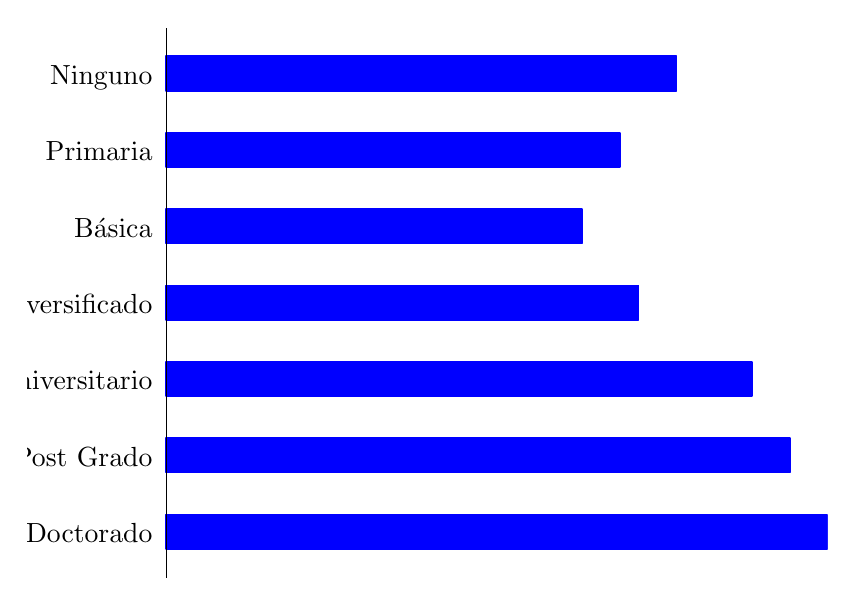
\begin{tikzpicture}[x=1pt,y=1pt]  % Created by tikzDevice version 0.10.1 on 2016-02-29 14:47:24
% !TEX encoding = UTF-8 Unicode
\definecolor{fillColor}{RGB}{255,255,255}
\path[use as bounding box,fill=fillColor,fill opacity=0.00] (0,0) rectangle (289.08,198.74);
\begin{scope}
\path[clip] (  0.00,  0.00) rectangle (289.08,198.74);

\path[] (  0.00,  0.00) rectangle (289.08,198.74);
\end{scope}
\begin{scope}
\path[clip] (  0.00,  0.00) rectangle (289.08,198.74);

\path[] ( 50.00,  0.00) rectangle (289.08,198.74);

\path[] ( 50.00, 16.56) --
	(289.08, 16.56);

\path[] ( 50.00, 44.16) --
	(289.08, 44.16);

\path[] ( 50.00, 71.77) --
	(289.08, 71.77);

\path[] ( 50.00, 99.37) --
	(289.08, 99.37);

\path[] ( 50.00,126.97) --
	(289.08,126.97);

\path[] ( 50.00,154.58) --
	(289.08,154.58);

\path[] ( 50.00,182.18) --
	(289.08,182.18);
\definecolor{drawColor}{RGB}{0,0,255}
\definecolor{fillColor}{RGB}{0,0,255}

\path[draw=drawColor,line width= 0.6pt,line join=round,fill=fillColor] ( 50.00, 10.35) rectangle (289.08, 22.77);

\path[draw=drawColor,line width= 0.6pt,line join=round,fill=fillColor] ( 50.00, 37.95) rectangle (275.42, 50.38);

\path[draw=drawColor,line width= 0.6pt,line join=round,fill=fillColor] ( 50.00, 65.56) rectangle (261.76, 77.98);

\path[draw=drawColor,line width= 0.6pt,line join=round,fill=fillColor] ( 50.00, 93.16) rectangle (220.77,105.58);

\path[draw=drawColor,line width= 0.6pt,line join=round,fill=fillColor] ( 50.00,120.76) rectangle (200.28,133.19);

\path[draw=drawColor,line width= 0.6pt,line join=round,fill=fillColor] ( 50.00,148.37) rectangle (213.94,160.79);

\path[draw=drawColor,line width= 0.6pt,line join=round,fill=fillColor] ( 50.00,175.97) rectangle (234.43,188.39);
\definecolor{drawColor}{RGB}{0,0,0}

\path[draw=drawColor,line width= 0.1pt,line join=round] ( 50.00,  0.00) -- ( 50.00,198.74);

\path[] ( 50.00,  0.00) rectangle (289.08,198.74);
\end{scope}
\begin{scope}
\path[clip] (  0.00,  0.00) rectangle (289.08,198.74);

\path[] ( 50.00,  0.00) --
	( 50.00,198.74);
\end{scope}
\begin{scope}
\path[clip] (  0.00,  0.00) rectangle (289.08,198.74);
\definecolor{drawColor}{RGB}{0,0,0}

\node[text=drawColor,anchor=base east,inner sep=0pt, outer sep=0pt, scale=  1.00] at ( 45.05, 12.65) {Doctorado};

\node[text=drawColor,anchor=base east,inner sep=0pt, outer sep=0pt, scale=  1.00] at ( 45.05, 40.26) {Post Grado};

\node[text=drawColor,anchor=base east,inner sep=0pt, outer sep=0pt, scale=  1.00] at ( 45.05, 67.86) {Universitario};

\node[text=drawColor,anchor=base east,inner sep=0pt, outer sep=0pt, scale=  1.00] at ( 45.05, 95.46) {Diversificado};

\node[text=drawColor,anchor=base east,inner sep=0pt, outer sep=0pt, scale=  1.00] at ( 45.05,123.07) {Básica};

\node[text=drawColor,anchor=base east,inner sep=0pt, outer sep=0pt, scale=  1.00] at ( 45.05,150.67) {Primaria};

\node[text=drawColor,anchor=base east,inner sep=0pt, outer sep=0pt, scale=  1.00] at ( 45.05,178.27) {Ninguno};
\end{scope}
\begin{scope}
\path[clip] (  0.00,  0.00) rectangle (289.08,198.74);

\path[] ( 47.25, 16.56) --
	( 50.00, 16.56);

\path[] ( 47.25, 44.16) --
	( 50.00, 44.16);

\path[] ( 47.25, 71.77) --
	( 50.00, 71.77);

\path[] ( 47.25, 99.37) --
	( 50.00, 99.37);

\path[] ( 47.25,126.97) --
	( 50.00,126.97);

\path[] ( 47.25,154.58) --
	( 50.00,154.58);

\path[] ( 47.25,182.18) --
	( 50.00,182.18);
\end{scope}
  \end{tikzpicture}}{Instituto Nacional de Estadística, con datos del Ministerio de Educación}

\cajota{Deserción en los departamentos}{Los departamentos con las menores tasas de deserción en primaria fueron:  Sacatepéquez 2.0\%, Quetzaltenango 1.9\% y Chimaltenango 1.7\%,
	
	 Los departamentos con las mayores tasas de deserción en primaria en el 2013 fueron: Petén 7.9\%, Zacapa 5.9\% e Izabal 5.7\%. En el departamento de Guatemala la tasa de deserción fue de 2.5\%.	}{Tasa de deserción del ciclo de educación primaria}{Por departamento, año 2014, en porcentaje}{\includegraphics[width=52\cuadri]{graficas/primaria/1_22.pdf}}{Instituto Nacional de Estadística, con datos del Ministerio de Educación}




\cajita{Aprobación}{La tasa de aprobación en primaria se refiere a la cantidad de alumnos que culminaron y aprobaron el ciclo lectivo.
	
	En el año 2009 fue de 86.4\% y en el año 2014 fue de 87.5\%, presentó un aumento en 1.1 puntos porcentuales.}{Tasa de aprobación del ciclo de educación primaria}{República de Guatemala, serie histórica, en porcentaje}{\ \\[0mm]\begin{tikzpicture}[x=1pt,y=1pt]  % Created by tikzDevice version 0.9 on 2016-02-29 21:54:12
% !TEX encoding = UTF-8 Unicode
\definecolor{fillColor}{RGB}{255,255,255}
\path[use as bounding box,fill=fillColor,fill opacity=0.00] (0,0) rectangle (289.08,198.74);
\begin{scope}
\path[clip] (  0.00,  0.00) rectangle (289.08,198.74);

\path[] (  0.00,  0.00) rectangle (289.08,198.74);
\end{scope}
\begin{scope}
\path[clip] (  0.00,  0.00) rectangle (289.08,198.74);

\path[] ( -0.52, 15.61) rectangle (280.54,191.48);

\path[] (  0.00, 52.67) --
	(280.54, 52.67);

\path[] (  0.00,110.78) --
	(280.54,110.78);

\path[] (  0.00,168.90) --
	(280.54,168.90);

\path[] (  0.00, 23.61) --
	(280.54, 23.61);

\path[] (  0.00, 81.72) --
	(280.54, 81.72);

\path[] (  0.00,139.84) --
	(280.54,139.84);

\path[] ( 26.68, 15.61) --
	( 26.68,191.48);

\path[] ( 72.01, 15.61) --
	( 72.01,191.48);

\path[] (117.35, 15.61) --
	(117.35,191.48);

\path[] (162.68, 15.61) --
	(162.68,191.48);

\path[] (208.01, 15.61) --
	(208.01,191.48);

\path[] (253.34, 15.61) --
	(253.34,191.48);
\definecolor{drawColor}{RGB}{0,0,255}

\path[draw=drawColor,line width= 1.7pt,line join=round] ( 26.68,177.04) --
	( 72.01,169.37) --
	(117.35,167.45) --
	(162.68,172.91) --
	(208.01,178.08) --
	(253.34,183.49);
\definecolor{drawColor}{RGB}{0,0,0}

\node[text=drawColor,anchor=base,inner sep=0pt, outer sep=0pt, scale=  1.02] at ( 26.68,181.01) {86.4};

\node[text=drawColor,anchor=base west,inner sep=0pt, outer sep=0pt, scale=  1.02] at ( 72.01,173.34) {85.1};

\node[text=drawColor,anchor=base,inner sep=0pt, outer sep=0pt, scale=  1.02] at (117.35,155.54) {84.8};

\node[text=drawColor,anchor=base east,inner sep=0pt, outer sep=0pt, scale=  1.02] at (159.55,172.91) {85.7};

\node[text=drawColor,anchor=base east,inner sep=0pt, outer sep=0pt, scale=  1.02] at (204.88,178.08) {86.6};

\node[text=drawColor,anchor=base,inner sep=0pt, outer sep=0pt, scale=  1.02] at (253.34,187.46) {87.5};

\path[draw=drawColor,line width= 0.1pt,line join=round] (  0.00, 23.61) -- (280.54, 23.61);

\path[] ( -0.52, 15.61) rectangle (280.54,191.48);
\end{scope}
\begin{scope}
\path[clip] (  0.00,  0.00) rectangle (289.08,198.74);

\path[] (  0.00, 15.61) --
	(280.54, 15.61);
\end{scope}
\begin{scope}
\path[clip] (  0.00,  0.00) rectangle (289.08,198.74);

\path[] ( 26.68, 12.86) --
	( 26.68, 15.61);

\path[] ( 72.01, 12.86) --
	( 72.01, 15.61);

\path[] (117.35, 12.86) --
	(117.35, 15.61);

\path[] (162.68, 12.86) --
	(162.68, 15.61);

\path[] (208.01, 12.86) --
	(208.01, 15.61);

\path[] (253.34, 12.86) --
	(253.34, 15.61);
\end{scope}
\begin{scope}
\path[clip] (  0.00,  0.00) rectangle (289.08,198.74);
\definecolor{drawColor}{RGB}{0,0,0}

\node[text=drawColor,anchor=base,inner sep=0pt, outer sep=0pt, scale=  1.00] at ( 26.68,  2.85) {2009};

\node[text=drawColor,anchor=base,inner sep=0pt, outer sep=0pt, scale=  1.00] at ( 72.01,  2.85) {2010};

\node[text=drawColor,anchor=base,inner sep=0pt, outer sep=0pt, scale=  1.00] at (117.35,  2.85) {2011};

\node[text=drawColor,anchor=base,inner sep=0pt, outer sep=0pt, scale=  1.00] at (162.68,  2.85) {2012};

\node[text=drawColor,anchor=base,inner sep=0pt, outer sep=0pt, scale=  1.00] at (208.01,  2.85) {2013};

\node[text=drawColor,anchor=base,inner sep=0pt, outer sep=0pt, scale=  1.00] at (253.34,  2.85) {2014};
\end{scope}
  \end{tikzpicture}}{Instituto Nacional de Estadística, con datos del Ministerio de Educación}

\cajita{Aprobación por sexo}{La tasa de aprobación en primaria por sexo, representa el 86.3\% para hombres y 88.8\% para las mujeres.}{Tasa de aprobación del ciclo de educación primaria, por sexo}{República de Guatemala, año 2014, en porcentaje}{\ \\[0mm]\begin{tikzpicture}[x=1pt,y=1pt]  \input{graficas/primaria/1_24.tex}  \end{tikzpicture}}{Instituto Nacional de Estadística, con datos del Ministerio de Educación}

\cajota{Aprobación en los departamentos}{El mapa muestra en color celeste los departamentos con las menores tasas de aprobación en primaria: Jalapa 83.0\%, Chiquimula 81.7\% y Alta Verapaz 78.6\%.
	
	  Los departamentos con las mayores tasas  de aprobación en primaria fueron: Guatemala 94.3\%, Sacatepéquez 90.7\% y  El Progreso 90.6\%. }{Tasa de aprobación del ciclo de educación primaria}{Por departamento, año 2014, en porcentaje}{\includegraphics[width=52\cuadri]{graficas/primaria/1_25.pdf}}{Instituto Nacional de Estadística, con datos del Ministerio de Educación}



